
\documentclass[oneside,a4paper]{book}
%\pagestyle{headings}


%=============================================================================
%crypto packages
\usepackage[labelfont=bf,labelsep=period]{caption}
\usepackage[nodayofweek]{datetime}
\usepackage[margin=2.5cm]{geometry}
\usepackage{numbertabbing}
\usepackage{subcaption}
\usepackage{pgfplots}
\pgfplotsset{compat=1.18}

%benefri packages
\usepackage{enumitem}
\usepackage{amsthm}
\usepackage{xspace}
\usepackage{float}
\usepackage{ifthen}
\usepackage{amsbsy}
\usepackage{amssymb}
\usepackage{balance}
\usepackage{booktabs}
\usepackage{graphicx}
\usepackage{rotating}
\usepackage{multirow}
\usepackage{needspace}
\usepackage{microtype}
\usepackage{bold-extra}
\usepackage{varioref}
\usepackage{xcolor}
\usepackage{textcomp}
\usepackage{listings}
\usepackage[normalem]{ulem} %emphasize still italic
\usepackage{ucs}

\usepackage[utf8]{inputenc}
% \usepackage[htt]{hyphenat}
\usepackage{times}
\usepackage{url}
\usepackage{alltt}
\usepackage{amsmath}
\allowdisplaybreaks[2] 

\usepackage{xfrac}
%\usepackage{subfigure}
\usepackage{appendix}
\usepackage{stmaryrd}   % for the \shortuparrow
\usepackage[utopia]{quotchap}

\usepackage{setspace}
\usepackage[numbers, sort&compress]{natbib}
\usepackage{mdwlist}        % support for better spaced lists
% allows for temporary adjustment of side margins
\usepackage{chngpage}
\usepackage[normalem]{ulem} 

\newtheoremstyle{plain-boldhead}% name
  {\topsep}%      Space above
  {\topsep}%      Space below
  {\itshape}%     Body font
  {}%         Indent amount (empty = no indent, \parindent = para indent)
  {\bfseries}% Thm head font
  {.}%        Punctuation after thm head
  { }%     Space after thm head: " " = normal space; \newline = linebreak
  {\thmname{#1}\thmnumber{ #2}\thmnote{ (\bfseries #3)}}%    Thm head spec
\newtheoremstyle{definition-boldhead}% name
  {\topsep}%      Space above
  {\topsep}%      Space below
  {\normalfont}% Body font
  {}%         Indent amount (empty = no indent, \parindent = para indent)
  {\bfseries}% Thm head font
  {.}%        Punctuation after thm head
  { }%     Space after thm head: " " = normal space; \newline = linebreak
  {\thmname{#1}\thmnumber{ #2}\thmnote{ (\bfseries #3)}}%    Thm head spec
\theoremstyle{plain-boldhead}
\newtheorem{theorem}{Theorem}
\newtheorem{proposition}[theorem]{Proposition}
\newtheorem{lemma}[theorem]{Lemma}
\newtheorem{corollary}[theorem]{Corollary}
\newtheorem{claim}{Claim}[theorem]
\theoremstyle{definition-boldhead}
\newtheorem{definition}{Definition}
\newtheorem{remark}{Remark}
\newtheorem{example}{Example}

%%% control the date format %%%
\newdateformat{simple}{\THEDAY\ \monthname[\THEMONTH]\ \THEYEAR}
\simple

%%% algorithms float %%%
\floatstyle{ruled}
\newfloat{algo}{htbp}{algo}
\floatname{algo}{Algorithm}

\newfloat{module}{htbp}{module}
\floatname{module}{Module}

%%% short cuts %%%
\def \ifempty#1{\def\temp{#1} \ifx\temp\empty }
\renewcommand{\P}{\mathrm{P}}
\newcommand{\E}{\mathrm{E}}
\newcommand{\Var}{\mathrm{Var}}
\newcommand{\str}[1]{\textsc{#1}}
\newcommand{\var}[1]{\textit{#1}}
\newcommand{\op}[1]{\textsl{#1}}
\newcommand{\msg}[2]{\ensuremath{\ifempty{#2} [\str{#1}] \else [\str{#1}, {#2}] \fi}}
\newcommand{\tup}[1]{\ensuremath{\langle #1 \rangle}}
\newcommand{\event}[1]{\tup{\textit{#1}}}
\newcommand{\eventp}[2]{\mbox{\textsl{#1}(#2)}}
\newcommand{\instance}[1]{\textbf{instance}~\var{#1}}
\newcommand{\becomes}{\ensuremath{\leftarrow}}
\newcommand{\getsr}{{\:{\leftarrow{\hspace*{-3pt}\raisebox{.75pt}{$\scriptscriptstyle\$$}}}\:}}
\newcommand{\concat}{\ensuremath{\circ}}
\newcommand{\nil}{\ensuremath{\bot}}
\newcommand{\false}{\textsc{false}\xspace}
\newcommand{\true}{\textsc{true}\xspace}
\newcommand{\etal}{\emph{et al.}}

\DeclareMathOperator*{\argmax}{arg\,max}

%%% bb and cal charactres %%%
\newcommand{\BA}{\ensuremath{\mathbb{A}}\xspace}
\newcommand{\BB}{\ensuremath{\mathbb{B}}\xspace}
\newcommand{\BC}{\ensuremath{\mathbb{C}}\xspace}
\newcommand{\BD}{\ensuremath{\mathbb{D}}\xspace}
\newcommand{\BE}{\ensuremath{\mathbb{E}}\xspace}
\newcommand{\BF}{\ensuremath{\mathbb{F}}\xspace}
\newcommand{\BG}{\ensuremath{\mathbb{G}}\xspace}
\newcommand{\BH}{\ensuremath{\mathbb{H}}\xspace}
\newcommand{\BI}{\ensuremath{\mathbb{I}}\xspace}
\newcommand{\BJ}{\ensuremath{\mathbb{J}}\xspace}
\newcommand{\BK}{\ensuremath{\mathbb{K}}\xspace}
\newcommand{\BL}{\ensuremath{\mathbb{L}}\xspace}
\newcommand{\BM}{\ensuremath{\mathbb{M}}\xspace}
\newcommand{\BN}{\ensuremath{\mathbb{N}}\xspace}
\newcommand{\BO}{\ensuremath{\mathbb{O}}\xspace}
\newcommand{\BP}{\ensuremath{\mathbb{P}}\xspace}
\newcommand{\BQ}{\ensuremath{\mathbb{Q}}\xspace}
\newcommand{\BR}{\ensuremath{\mathbb{R}}\xspace}
\newcommand{\BS}{\ensuremath{\mathbb{S}}\xspace}
\newcommand{\BT}{\ensuremath{\mathbb{T}}\xspace}
\newcommand{\BU}{\ensuremath{\mathbb{U}}\xspace}
\newcommand{\BV}{\ensuremath{\mathbb{V}}\xspace}
\newcommand{\BW}{\ensuremath{\mathbb{W}}\xspace}
\newcommand{\BX}{\ensuremath{\mathbb{X}}\xspace}
\newcommand{\BY}{\ensuremath{\mathbb{Y}}\xspace}
\newcommand{\BZ}{\ensuremath{\mathbb{Z}}\xspace}

\newcommand{\CA}{\ensuremath{\mathcal{A}}\xspace}
\newcommand{\CB}{\ensuremath{\mathcal{B}}\xspace}
\newcommand{\CC}{\ensuremath{\mathcal{C}}\xspace}
\newcommand{\CD}{\ensuremath{\mathcal{D}}\xspace}
\newcommand{\CE}{\ensuremath{\mathcal{E}}\xspace}
\newcommand{\CF}{\ensuremath{\mathcal{F}}\xspace}
\newcommand{\CG}{\ensuremath{\mathcal{G}}\xspace}
\newcommand{\CH}{\ensuremath{\mathcal{H}}\xspace}
\newcommand{\CI}{\ensuremath{\mathcal{I}}\xspace}
\newcommand{\CJ}{\ensuremath{\mathcal{J}}\xspace}
\newcommand{\CK}{\ensuremath{\mathcal{K}}\xspace}
\newcommand{\CL}{\ensuremath{\mathcal{L}}\xspace}
\newcommand{\CM}{\ensuremath{\mathcal{M}}\xspace}
\newcommand{\CN}{\ensuremath{\mathcal{N}}\xspace}
\newcommand{\CO}{\ensuremath{\mathcal{O}}\xspace}
\newcommand{\CP}{\ensuremath{\mathcal{P}}\xspace}
\newcommand{\CQ}{\ensuremath{\mathcal{Q}}\xspace}
\newcommand{\CR}{\ensuremath{\mathcal{R}}\xspace}
\newcommand{\CS}{\ensuremath{\mathcal{S}}\xspace}
\newcommand{\CT}{\ensuremath{\mathcal{T}}\xspace}
\newcommand{\CU}{\ensuremath{\mathcal{U}}\xspace}
\newcommand{\CV}{\ensuremath{\mathcal{V}}\xspace}
\newcommand{\CW}{\ensuremath{\mathcal{W}}\xspace}
\newcommand{\CX}{\ensuremath{\mathcal{X}}\xspace}
\newcommand{\CY}{\ensuremath{\mathcal{Y}}\xspace}
\newcommand{\CZ}{\ensuremath{\mathcal{Z}}\xspace}

%%% annotations %%%
\providecommand{\note}[1]{[[\textsf{#1}]]}
\providecommand{\todo}[1]{\note{TODO: #1}}

%%% example variable abbreviations (delete or modify) %%% 
\newcommand\lastts{\var{lastts}\xspace}
\newcommand\nextts{\var{nextts}\xspace}
\newcommand\trusted{\var{trusted}\xspace}
\newcommand\newepoch{\var{newepoch}\xspace}
\newcommand\leader{\var{leader}\xspace}
\newcommand\ts{\var{ts}\xspace}

\newcommand\received{\var{received}\xspace}
\newcommand\collected{\var{collected}\xspace}
\newcommand\val {\var{val}\xspace}
\newcommand\sent {\var{sent}\xspace}
\newcommand\ws {\var{ws}\xspace}
\newcommand\written {\var{written}\xspace}
\newcommand\decided {\var{decided}\xspace}
\newcommand\accepted {\var{accepted}\xspace}
\newcommand\wrote {\var{wrote}\xspace}
\newcommand \round{\var{round}\xspace}

\newcommand{\comment}[1]{\textcolor{blue}{Comment: #1}}


% constants

\newcounter{qcounter}

% commands
\newcommand{\n}{$\cdot$}
\newcommand{\y}{\checkmark}
\newcommand{\subscript}[1]{$_{\textrm{\footnotesize{#1}}}$}
\newcommand{\superscript}[1]{$^{\textrm{\footnotesize{#1}}}$}
\newcommand{\vertical}[1]{\raisebox{-4em}{\begin{sideways}{#1}\end{sideways}}}

\newboolean{showedits}
\setboolean{showedits}{true} % toggle to show or hide edits
\ifthenelse{\boolean{showedits}}
{
       \newcommand{\ugh}[1]{\textcolor{red}{\uwave{#1}}} % please rephrase
       \newcommand{\ins}[1]{\textcolor{blue}{\uline{#1}}} % please insert
       \newcommand{\del}[1]{\textcolor{red}{\sout{#1}}} % please delete
       \newcommand{\chg}[2]{\textcolor{red}{\sout{#1}}{\ra}\textcolor{blue}{\uline{#2}}} % please change
}{
       \newcommand{\ugh}[1]{#1} % please rephrase
       \newcommand{\ins}[1]{#1} % please insert
       \newcommand{\del}[1]{} % please delete
       \newcommand{\chg}[2]{#2}
}


% ============================================================================
% Put edit comments in a really ugly standout display

\usepackage{xcolor}
\usepackage[normalem]{ulem}
\newcommand{\ra}{$\rightarrow$}


% comments \nb{label}{color}{text}
\newboolean{showcomments}
\setboolean{showcomments}{true}
\ifthenelse{\boolean{showcomments}}
    {\newcommand{\nb}[3]{
        {\colorbox{#2}{\bfseries\sffamily\scriptsize\textcolor{white}{#1}}}
        {\textcolor{#2}{\sf\small$\blacktriangleright$\textit{#3}$\blacktriangleleft$}}}
     \newcommand{\version}{\emph{\scriptsize$-$Id$-$}}
%	 \newcommand{\ugh}[1]{\textcolor{red}{\uwave{#1}}} % please rephrase
%	 \newcommand{\ins}[1]{\textcolor{blue}{\uline{#1}}} % please insert
%	 \newcommand{\del}[1]{\textcolor{red}{\sout{#1}}} % please delete
%	 \newcommand{\chg}[2]{\textcolor{red}{\sout{#1}}{\ra}\textcolor{blue}{\uline{#2}}} % please change
	 \newcommand{\chk}[1]{\textcolor{ForestGreen}{#1}} % changed, please check
	}
    {\newcommand{\nb}[3]{}
     \newcommand{\version}{}
	\newcommand{\chk}[1]{} % changed, please check
	}

% ============================================================================
% Make quotes be italic
\renewenvironment{quote}
    {\list{}{\rightmargin\leftmargin}%
     \item\relax\begin{it}}
    {\end{it}\endlist}

\newcommand{\ttimes}{\ensuremath{\times}}

%=============================================================================

\newcommand{\needlines}[1]{\Needspace{#1\baselineskip}}

% source code
\usepackage{xcolor}
\usepackage{textcomp}
\usepackage{listings}
\definecolor{source}{gray}{0.9}
\lstset{
	language={},
	% characters
	tabsize=3,
	upquote=true,
	escapechar={!},
	keepspaces=true,
	breaklines=false,
	alsoletter={:},
	breakautoindent=true,
	columns=fullflexible,
	showstringspaces=false,
	basicstyle=\footnotesize\ttfamily,
	% background
	frame=single,
    framerule=0pt,
	backgroundcolor=\color{source},
	% numbering
	numbersep=5pt,
	numberstyle=\tiny,
	numberfirstline=true,
	% captioning
	captionpos=b,
	numberbychapter=false,
	% formatting (html)
	moredelim=[is][\textbf]{<b>}{</b>},
	moredelim=[is][\textit]{<i>}{</i>},
	moredelim=[is][\uline]{<u>}{</u>}}
\newcommand{\ct}{\lstinline[backgroundcolor=\color{white},basicstyle=\footnotesize\ttfamily]}
\newcommand{\lct}[1]{{\small\tt #1}}


%----------------------------------------------------------------------------
% references
\newcommand{\tabref}[1]{\hyperref[{tab:#1}]{Table~\ref*{tab:#1}}}
\newcommand{\figref}[1]{\hyperref[{fig:#1}]{Figure~\ref*{fig:#1}}}
\newcommand{\secref}[1]{\hyperref[{sec:#1}]{Section~\ref*{sec:#1}}}
\newcommand{\lstref}[1]{\hyperref[{lst:#1}]{Listing~\ref*{lst:#1}}}
\newcommand{\charef}[1]{\hyperref[{cha:#1}]{Chapter~\ref*{cha:#1}}}
%----------------------------------------------------------------------------

% abbreviations
\tracingcolors 4
\setcounter{tocdepth}{3}
\setcounter{secnumdepth}{3}
\newcommand{\ie}{\emph{i.e.,}\xspace}
\newcommand{\eg}{\emph{e.g.,}\xspace}
\newcommand{\etc}{\emph{etc.}\xspace}


\newcommand{\newevenside}{
	\ifthenelse{\isodd{\thepage}}{\newpage}{
	\newpage
        \phantom{placeholder} % doesn't appear on page
	\thispagestyle{empty} % if want no header/footer
	\newpage
	}
}

\def\stretchfactor{1}
\newcommand{\mychapter}[1]{\setstretch{1}
    \chapter{#1}\setstretch{\stretchfactor}}

%----------------------------------------------------------------------------
\newcommand{\lessSpace}{\vspace{-1em}}
\DeclareGraphicsExtensions{.pdf,.png}
\graphicspath{{images/}}
\newcommand{\fig}[4]{
	\begin{figure}[#1]
		\centering
		\includegraphics[width=#2\textwidth]{#3}
		\lessSpace
		\caption{\label{fig:#3}#4}
	\end{figure}}

% ===========================================================================


\newcommand{\thesistitle}{APBFT}
\newcommand{\thesisauthor}{Bernhard Jonathan}
\newcommand{\thesisleiter}{Christian Cachin}
\newcommand{\thesisasst}{Juan Villacis \& Michael Senn}
\newcommand{\thesissubtitle}{Adapting the PBFT Consensus Algorithm to the Asymmetric Trust Setting}
\newcommand{\thesisdate}{August 2025}



% ===========================================================================

\usepackage[ colorlinks=true, urlcolor=black, linkcolor=black,
			citecolor=black, bookmarksnumbered=true, bookmarks=true,
			plainpages=false,
			pdftitle={\thesistitle}, pdfauthor={\thesisauthor},
			pdfsubject={\thesissubtitle}, pdfpagelabels]{hyperref}

\newcommand{\hrref}[2]{\hyperref}
% ===========================================================================
% ===========================================================================


% D O C U M E N T
% % % % % % % % % % % % % % % % % % % % % % % % % % % % % % % % % %
\pagestyle{plain}
\begin{document}

% T I T L E
% % % % % % % % % % % % % % % % % % % % % % % % % % % % % % % % % %
\begin{titlepage}  
  \begin{center}  
  
  \begin{figure}[t]  
  \vspace*{-2cm}        % to move header logo at the top 
  \center{
\includegraphics[scale=0.2]{logos/MSc_quer.png}}
  \vspace{0.4in}     
  \end{figure}

    \thispagestyle{empty}
    
    {\bfseries\Huge \thesistitle \par
    \Large \vspace{0.1in} \thesissubtitle \par}

    \vspace{0.3in} 
    \LARGE{\textbf{Master Thesis} \\}
    \vspace{0.4in}

    {\Large \thesisauthor}
    
    \vspace{0.3in}
    {\Large Universität Freiburg \par}
%    {\Large Philosophisch-naturwissenschaftlichen Fakult\"{a}t \\
%            der Universit\"{a}t Bern \par}

    
    
    \vfill
    {\Large \thesisdate \par}

     \vspace{0.6in}

    % === Supervisor & Assistants section ===
    {\large
     Prof. Dr. Christian Cashin \par
     Juan Villacis \par
     Michael Senn
     
     
    }

    \vspace{0.3in}

    % === Additional bottom text ===
    {\large
    Cryptology and Data Security Group \par
    Institute of Computer Science \par
    University of Bern, Switzerland \par
    }
  

  \vspace{0.9in}
 
  % === Logos ==============================================     
  \begin{figure}[htp]
    \centering
    
\includegraphics[scale=0.30]{logos/UNI_Bern.png}\hfill
    
\includegraphics[scale=0.30]{logos/UNI_Neuenburg.png}\hfill
    
\includegraphics[scale=0.80]{logos/UNI_Fribourg.png}
  \end{figure}
  % === // Logos ===========================================    


  \end{center}

\end{titlepage}


% A B S T R A C T
% % % % % % % % % % % % % % % % % % % % % % % % % % % % % % % % % %
\chapter*{\centering Abstract}
\begin{quotation}
\noindent 
Consensus protocols are fundamental to distributed computing, enabling processes to agree on a single value even in the presence of faults. Traditional consensus mechanisms, such as Paxos, PBFT, HotStuff, and Tendermint, assume a symmetric trust model where all nodes share uniform assumptions about fault tolerance. While effective in controlled environments, this assumption often limits applicability in large-scale, decentralized, or geo-distributed networks, where nodes may hold heterogeneous trust views.

This thesis investigates consensus under asymmetric trust, where each node specifies its own fail-prone sets. We present the first empirical evaluation of two consensus paradigms adapted to this setting: a leader-driven PBFT variant (PAPBFT) and Asymmetric Randomized Consensus, a fully asynchronous randomized consensus protocol. Our experiments demonstrate that PAPBFT achieves low latency in fault-free scenarios but is sensitive to faulty leaders, whereas the randomized protocol maintains stable performance regardless of faults.

To make such protocols practical, we examine the computational complexity of key quorum-related tasks and prove that enumerating the tolerated system of an asymmetric quorum system, which a key component of several algorithms, is NP-hard. We address this challenge by introducing the superset recognizer abstraction, and show that an efficient recognizer for a quorum system can be transformed into recognizers for both its kernel system and its tolerated system. This allows the algorithms to be implemented entirely on top of quorum superset recognizers, avoiding the need to explicitly enumerate these complex structures.

Building on prior work, we extend the PBFT algorithm with a leader-change primitive tailored for asymmetric trust and propose a novel asymmetric variant of the PBFT consensus mechanism that manages unequal role assignments among nodes. We provide a formal correctness proof of our PBFT variant, ensuring both safety and liveness in asymmetric trust environments. These contributions establish a practical foundation for reliable and efficient consensus in heterogeneous distributed systems.

%Christian Cachin, Cryptology and Data Security Group, Institute of Computer Science, University of Bern

%Juan Villacis, Cryptology and Data Security Group, Institute of Computer Science, University of Bern

%Michael Senn, Cryptology and Data Security Group, Institute of Computer Science, University of Bern
\end{quotation}
\clearpage


% C O N T E N T S 
% % % % % % % % % % % % % % % % % % % % % % % % % % % % % % % % % % % % % % % %
\tableofcontents

%%%%%%%%%%%%%%%%%%%%%%%%%%%%%%%%%%
%%%% NEW CHAPTER %%%%%%%%%%%%%%%%%%%%%
%%%%%%%%%%%%%%%%%%%%%%%%%%%%%%%%%%
\chapter{Introduction}
\label{cha:introduction}
The consensus problem is a core abstraction in distributed computing, requiring processes to agree on a single value among those proposed, even in the presence of faults. It underpins systems that require consistent transaction ordering, as repeated instances can be used to build a global sequence of decisions. Protocols such as \textsc{Paxos}~\cite{DBLP:journals/tocs/Lamport98}, \textsc{PBFT}~\cite{DBLP:conf/osdi/CastroL99}, \textsc{HotStuff}~\cite{DBLP:conf/podc/YinMRGA19}, and \textsc{Tendermint}~\cite{DBLP:journals/corr/abs-1807-04938} are well-established consensus mechanisms in practice, forming the foundation of many replicated services and permissioned blockchain systems.

These protocols are built on top of the \emph{symmetric trust model}, where all nodes share a uniform assumption about the number and type of faults the system must tolerate. Typically, this is captured by a fixed threshold, e.g., the assumption that at most $f$ out of $n$ nodes are Byzantine, meaning they may behave in arbitrary or malicious ways. Under this assumption, quorum systems are constructed such that every quorum has sufficient overlap with others to guarantee both \emph{safety} and \emph{liveness} properties.

This threshold-based model can be more generally captured by the framework of \emph{Byzantine quorum systems (BQS)}~\cite{DBLP:journals/dc/MalkhiR98}. Instead of relying on numerical thresholds, BQS define a set of \emph{fail-prone sets}: collections of nodes that might fail together. A quorum system is then a set of node subsets that intersect with one another and contain a sufficient number of correct processes. In the symmetric BQS model, all nodes share the same quorums and fail-prone sets, preserving the assumption of a homogeneous trust structure.

However, this symmetric trust assumption can become a significant limitation in real-world systems. In large-scale, geo-distributed, or decentralized networks, participants may have very different views of which nodes they consider trustworthy. Nodes operated by independent entities often cannot agree on a global fault assumption.

To address these limitations, BQS have been extended to support \emph{asymmetric trust}. In this setting, as introduced by Damg\aa rd et al.~\cite{DBLP:conf/asiacrypt/DamgardDFN07} and later refined by Alpos et al.~\cite{DBLP:journals/dc/AlposCTZ24}, each node specifies its own view of fail-prone sets, reflecting its local trust assumptions. 

Zanolini~\cite{Zanolini2023} introduced two consensus algorithms for the asymmetric trust setting: a variant of the PBFT algorithm as proposed by Cachin et al.~\cite{DBLP:books/daglib/0025983}, and a randomized consensus algorithm based on the work of Mostéfaoui et al.~\cite{DBLP:journals/jacm/MostefaouiMR15}. However, Zanolini neither provides an implementation of the proposed algorithms nor specifies the full PBFT mechanism, leaving, in particular, the liveness mechanism open. Building on this foundation, we complete Zanolini’s PBFT variant with a leader-change primitive tailored to the asymmetric trust setting, enabling its practical execution. We implement both of Zanolini’s algorithms and empirically evaluate their performance. Furthermore, we propose a novel asymmetric variant of PBFT and provide a formal proof of its correctness.

The remainder of this thesis is structured as follows.

\begin{itemize}
    \item \textbf{Chapter 2} discusses related work, particularly other consensus protocols that address asymmetric trust.
    \item \textbf{Chapter 3} presents the preliminaries, introducing the system model and quorum systems.
    \item \textbf{Chapter 4} details hardness results related to the computation of guilds in asymmetric quorum systems and discusses how to efficiently operationalize the reviewed quorum-based algorithms.
    \item \textbf{Chapter 5} reviews the Asymmetric Randomized Consensus algorithm.
    \item \textbf{Chapter 6} examines an asymmetric version of PBFT and introduces a novel variation of the protocol.
    \item \textbf{Chapter 7} presents the empirical evaluation of the two reviewed algorithms.
    \item \textbf{Chapter 8} outlines future work, discussing potential extensions and open questions.
    \item \textbf{Chapter 9} concludes the thesis, summarizing the results.
\end{itemize}

\chapter{Related Work}

The study of asymmetric trust in distributed consensus has been formalized through several foundational works. Damg\aa rd et al.~\cite{DBLP:conf/asiacrypt/DamgardDFN07} were the first to introduce the notion of asymmetric trust, laying the theoretical groundwork for subsequent research. Building on this foundation, Alpos et al.~\cite{DBLP:journals/dc/AlposCTZ24} formalized asymmetric trust as a generalization of symmetric Byzantine quorum systems~\cite{DBLP:journals/dc/MalkhiR98}, extending classical consistency and availability properties to a more flexible setting. In their framework, they also introduced the concept of a guild, a subset of correct nodes whose presence ensures system progress, and proved that their proposed consensus algorithms satisfy both safety and liveness under this model.

Subsequently, Li et al.\cite{DBLP:conf/wdag/LiCL23} showed that consistency and availability alone are insufficient to guarantee consensus in asymmetric trust environments, emphasizing the necessity of the guild condition identified by Alpos et al. They also developed their own model of asymmetric Byzantine quorum systems, derived from the Federated Byzantine Agreement System (FBAS) used in Stellar~\cite{stellarPap}. In this formulation, quorum system properties are defined relative to a fixed set of predetermined Byzantine processes. By contrast, the Alpos et al.\cite{DBLP:journals/dc/AlposCTZ24} approach defines these properties in terms of the fail-prone system introduced by Damg\aa rd et al.~\cite{DBLP:conf/asiacrypt/DamgardDFN07}, which leads to a more natural expression of the consistency property. This formulation accommodates executions in which the quorums of correct processes, with incorrect trust assumptions, need not intersect in a correct process with the quorums of its peers. Such scenarios cannot be expressed in Li et al.’s~\cite{DBLP:conf/wdag/LiCL23} formalism, where the consistency property requires the quorums of all correct processes to intersect in at least one correct process.

Amores-Sesar et al.~\cite{DBLP:journals/corr/abs-2505-17891} present the first DAG-based asymmetric consensus protocol, which generalizes the renowned DAG-Rider~\cite{DBLP:conf/podc/KeidarKNS21} algorithm using the same formal framework adopted in this work. This work builds directly on the model developed by Alpos et al.~\cite{DBLP:journals/dc/AlposCTZ24}.

In a somewhat independent line, Heterogeneous Paxos~\cite{DBLP:journals/corr/abs-2011-08253} generalizes Byzantine Paxos to settings with non-uniform trust. A further generalization of the protocol is that it allows learners to also operate under heterogeneous fault models. To capture these assumptions, the authors introduce the concept of a learner graph, where each learner is represented as a node labeled with its individual quorum system, the sets of validators it trusts to reach a decision. Edges between learners are labeled with safe sets, which specify the subsets of non-Byzantine nodes required to ensure that connected learners agree on their decision value.

Ripple~\cite{ripple_consensus_whitepaper,DBLP:journals/corr/abs-2011-14816} and Stellar~\cite{stellarPap} are two of the most prominent blockchain systems built on asymmetric trust assumptions, enabling open-ended membership without requiring a globally agreed-upon validator set. Ripple requires each node to maintain a static \emph{Unique Node List} (UNL), a list of trusted validators. A node only considers messages from nodes in its UNL and regards a transaction as validated if a sufficient proportion of those validators approve it. However, in practice, Ripple exhibits a relatively centralized structure: new participants are given a default UNL, which they can customize, but are discouraged from doing so, as poor choices could compromise the system’s safety guarantees~\cite{stellarPap}.

Stellar builds on and generalizes Ripple’s approach by introducing the concept of a Federated Byzantine Agreement System (FBAS). In Stellar, each node defines one or more quorum slices, subsets of nodes it trusts to reach consensus. These slices collectively give rise to quorums, which are sets of nodes that contain a quorum slice for each of their members. The structure of quorum slices and quorums in Stellar resembles the quorum systems and guilds discussed earlier. However, the two differ fundamentally in their properties, as the notion of quorum systems is grounded in the concept of fail-prone sets, whereas FBAS does not explicitly model the possible faulty processes in the system.

Both systems require careful configuration to ensure liveness: Ripple relies on timely communication and high UNL overlap~\cite{DBLP:journals/corr/abs-2011-14816}, while Stellar requires that nodes form quorum slices with adequate intersection and availability~\cite{DBLP:journals/corr/abs-1811-03642}. However, Stellar also assumes some level of network synchrony to guarantee progress.

Cobalt~\cite{DBLP:journals/corr/abs-1802-07240}, developed as a successor to Ripple’s protocol, retains the asymmetric trust model in which each node maintains a locally defined trusted set (similar to UNLs), but improves resilience by reducing the required overlap between them and operating under full asynchrony, without assuming bounded message delays.

\chapter{Preliminaries}

In this chapter, we introduce the system model and then review the notion of \emph{Asymmetric Byzantine Quorum Systems}, originally proposed by Damg\aa rd et al.~\cite{DBLP:conf/asiacrypt/DamgardDFN07} and later extended by Alpos et al.~\cite{DBLP:journals/dc/AlposCTZ24}. These systems offer a mathematical framework for formalizing trust assumptions in distributed environments and form the basis of all the protocols discussed in this work.

To build toward this generalization, we first review the classical notion of \emph{Symmetric Byzantine Quorum Systems}, introduced by Malkhi and Reiter~\cite{DBLP:journals/dc/MalkhiR98}, before moving on to the asymmetric setting.

\section{System Model}

\paragraph{Processes.} 
In this thesis, our attention is restricted to \emph{permissioned} systems of \(n\) processes, denoted by \(\CP = \{p_1, p_2, \dots, p_n\}\). The processes communicate with each other over a fully connected network.

\paragraph{Executions and Faults.} 
An execution starts with all processes in a special initial state. The processes then repeatedly trigger events, as soon as their guards are satisfied, changing the processes’ states. Every event executes as an atomic unit. Each event executed by some process is associated with a unique point in time \(t \in \mathbb{R}\), inducing a total order on the events. However, the processes do not have access to a global clock and are therefore unaware of this global ordering.

A process that follows its protocol throughout its execution is called \emph{correct}. Processes may \emph{crash} during execution or \emph{deviate arbitrarily} from their specification; such faulty processes are called \emph{Byzantine}.

\paragraph{Idealized Digital Signatures.} 
In the pseudocode, the cryptographic operation of generating digital signatures is abstracted into two operations, \(\op{sign}_i\) and \(\op{verify}_i\). Process \(p_i\) invokes \(\op{sign}_i\) by providing a object \(o\) as input and obtaining a signature \(\sigma \in \{0,1\}^*\) as output. Only \(p_i\) may invoke \(\op{sign}_i\). The operation \(\op{verify}_i\) may be called by any process: given an object \(o\) and a signature \(\sigma\), it returns \(\true\) if and only if \(p_i\) previously invoked \(\op{sign}_i(o)\) and produced \(\sigma\).

\paragraph{Timing Assumptions.} 
We consider two different timing models for message delays:

\begin{itemize}
  \item \textbf{Fully Asynchronous Model.}  Messages may be delayed by an unbounded amount of time but are guaranteed to eventually be delivered.
  \item \textbf{Partially Synchronous Model~\cite{DBLP:journals/jacm/DworkLS88}.}  The execution is divided into two phases. Before an unknown global stabilization time (\(\var{GST} \in \mathbb{R}\)), messages behave as in the fully asynchronous model. After \(\var{GST}\), every message sent is delivered within at most \(\Delta \in \mathbb{R}\) time units. Both \(\var{GST}\) and \(\Delta\) are unknown to the processes, and no messages are lost.
\end{itemize}

\section{Symmetric Byzantine Quorum System}
Given a set of processes \(\CP\), a \emph{fail-prone system} \(\CF \subseteq 2^{\CP}\) encodes the trust assumptions underlying the Byzantine quorum system. Each set \(F \in \CF\) represents a group of processes that might fail together during the execution of a distributed protocol. In essence, \(\CF\) specifies the failure patterns that processes in \(\CP\) are designed to tolerate.

A \emph{quorum system} \(\CQ \subseteq 2^{\CP}\) is a collection of subsets of \(\CP\) that guarantees both safety and liveness, under the assumption that failures conform to the structure defined by \(\CF\).

The safety property, known as the \textbf{Consistency Property}, ensures that any two quorums \(Q_1, Q_2 \in \CQ\) intersect in at least one correct process. This overlap guarantees that when two processes make decisions based on quorum information, they do so with input from at least one common, correct source, an essential property for avoiding divergence and maintaining global consistency.

The liveness property, referred to as the \textbf{Availability Property}, ensures that for any admissible failure set \(F \in \CF\), there exists at least one quorum \(Q \in \CQ\) that contains only correct processes. This ensures that progress remains possible despite faults.



\begin{definition}[Symmetric Byzantine Quorum System]
Let \(\CP\) be a set of processes, and \(\CF \subseteq 2^{\CP}\) a fail-prone system representing the possible sets of processes that may fail together.

A \textit{Byzantine quorum system} for \(\CF\) is a collection of quorums \(\CQ \subseteq 2^{\CP}\), where no quorum is contained in another, and each \(Q \in \CQ\) is called a quorum. The system satisfies the following two properties:

\begin{itemize}
\label{def:quo}
    \item \textbf{Consistency.} The intersection of any two quorums contains at least one correct process. Formally, for all \(Q_1, Q_2 \in \CQ\) and for all \(F \in \CF\),
    \[
    Q_1 \cap Q_2 \nsubseteq F.
    \]

    \item \textbf{Availability.} For every fail-prone set \(F \in \CF\), there exists a quorum \(Q \in \CQ\) that is disjoint from \(F\), i.e.,
    \[
    \forall F \in \CF, \exists Q \in \CQ : Q \cap F = \emptyset.
    \]
\end{itemize}
\end{definition}

The following definition introduces a conceptually simple yet powerful condition, known as the $Q^3$-condition, which determines whether a given fail-prone system $\CF$ can be complemented by a quorum system $\CQ$ that satisfies Definition~\ref{def:quo}.

\begin{definition}[$Q^3$-Condition]
     A fail-prone system $\CF$ satisfies the \emph{$Q^3$-condition}, abbreviated as
 $Q^3(\CF)$, whenever it holds that
 \[
 \forall F_1,F_2,F_3 \in \CF : F_1\cup F_2 \cup F_3 \neq \CP .
 \]
\end{definition}

Intuitively, the $Q^3$-condition states that no combination of three fail-prone sets can cover the entire set of processes. This condition captures a fundamental limit on the number of failures a quorum system can tolerate.

\begin{lemma}[Malkhi et al.~\cite{DBLP:journals/dc/MalkhiR98}]
     Given a fail-prone system $\CF$, a Byzantine quorum system for $\CF$ exists if and only if $Q^3(\CF)$.
\end{lemma}


\paragraph{Core Sets.} A core set is another important concept when designing distributed protocols. It refers to a minimal set of processes that is guaranteed to include at least one correct process in every execution. The formal definition is as follows:

\begin{definition}[Core Set]
Let \(\CP\) be a set of processes and \(\CF \subseteq 2^{\CP}\) a fail-prone system.

A \textit{core set} for \(\CF\) is a set \(C \subseteq \CP\) satisfying:

\begin{itemize}
    \item \textbf{Correctness Coverage.} The set \(C\) contains at least one correct process in any failure scenario, i.e., for all \(F \in \CF\),
    \[
    C \nsubseteq F \quad \text{or equivalently,} \quad C \cap (P \setminus F) \neq \emptyset.
    \]

    \item \textbf{Minimality.} No proper subset of \(C\) satisfies the above property. That is,
    \[
    \forall C' \subsetneq C, \exists F \in \CF : C' \subseteq F.
    \]
\end{itemize}
\end{definition}

We denote the collection of all core sets for \(\CF\) by \(\CC\).

\paragraph{Kernels.} Lastly, we introduce the notion of a \textit{kernel}, which generalizes the idea of a core set. A kernel is a minimal set of processes that intersects with every quorum in the system \(\CQ\). In this sense, every kernel includes at least one core set.

\begin{definition}[Kernel]
Let \(\CP\) be a set of processes, \(\CF \subseteq 2^{\CP}\) a fail-prone system, and \(\CQ \subseteq 2^{\CP}\) a quorum system.

A \textit{kernel} for \(\CQ\) is a set \(K \subseteq \CP\) such that:

\begin{itemize}
    \item \textbf{Quorum Intersection.} The kernel intersects every quorum, i.e.,
    \[
    \forall Q \in \CQ: K \cap Q \neq \emptyset.
    \]

    \item \textbf{Minimality.} No proper subset of \(K\) satisfies the above condition, i.e.,
    \[
    \forall K' \subsetneq K, \exists Q \in \CQ : K' \cap Q = \emptyset.
    \]
\end{itemize}
\end{definition}

We denote the set of all kernels of the quorum system \(\CQ\) by \(\CK\), also referred to as the \textit{kernel system}.

\section{Asymmetric Byzantine Quorum System}

The concept of a symmetric Byzantine quorum system can be generalized by allowing each process \(p_i\) to specify its own individual fail-prone system \(\CF_i \subseteq 2^{\CP}\), thereby expressing the potentially differing trust assumptions across processes. The array of these fail-prone systems, denoted by \(\BF = [\CF_1, \CF_2, \dots, \CF_n]\), is called the \emph{asymmetric fail-prone system}, and it encapsulates the system-wide asymmetric trust relationships within \(\CP\).

The properties required from a corresponding quorum system for $\BF$ are defined below. Observe that, for any pair of processes with correctly specified trust assumptions, meaning that in every execution the actual faulty processes are contained in their respective fail-prone sets, the asymmetric Byzantine quorum system provides the same consistency and availability guarantees as in the symmetric setting, among the quorums of these processes.

Before proceeding, we introduce the following notation, which will be useful in the formal definitions to come. For a given set $\CA \subseteq 2^{\CP}$ of subsets of $\CP$ the set $\CA^*$ is defined as $\CA^* = \{a \subseteq A  \big\vert  A \in \CA \}$, the set of all subsets of the sets in $\CA$. 

\begin{definition}[Asymmetric Byzantine Quorum System]
An \textit{asymmetric Byzantine quorum system} for an asymmetric fail-prone system \(\BF\) is an array of collections of sets \(\BQ = [\CQ_1, \dots, \CQ_n]\), where \(\CQ_i \subseteq 2^{\CP}\) for each \(i \in [1,n]\). The set \(\CQ_i\) is called the \emph{quorum system} of process \(p_i\), and any set \(Q_i \in \CQ_i\) is called a \emph{quorum} for \(p_i\).

The system satisfies the following properties:

\begin{itemize}
    \item \textbf{Consistency.} The intersection of any two quorums from any two processes contains at least one process that one of them trusts. Formally,
    \[
    \forall i, j \in [1,n],\, \forall Q_i \in \CQ_i,\, \forall Q_j \in \CQ_j,\, \forall F_{ij} \in \CF_i^* \cap \CF_j^* : \quad Q_i \cap Q_j \nsubseteq F_{ij}.
    \]

    \item \textbf{Availability.} For every process \(p_i\), and every fail-prone set \(F \in \CF_i\), there exists a quorum \(Q_i \in \CQ_i\) disjoint from \(F\), i.e.,
    \[
    \forall i \in [1,n],\, \forall F \in \CF_i,\, \exists Q_i \in \CQ_i : Q_i \cap F = \emptyset.
    \]
\end{itemize}
\end{definition}

The $B^3$-condition is the asymmetric counterpart of the $Q^3$-condition, and it expresses precisely how many faults an asymmetric quorum system can tolerate. The modifications made to its definition reflect the corresponding changes in the consistency property of the quorum system.

\begin{definition}[$B^3$-Condition]
    An asymmetric fail-prone system $\BF$ satisfies the \emph{$B^3$-condition}, abbreviated
 as $B^3(\BF)$, whenever it holds that
 \[
 \forall i, j \in [1,n], \forall F_i \in \CF_i , \forall F_j \in \CF_j,  \forall F_{ij} \in \CF_i^* \cap \CF_j^* : F_i \cup F_j \cup F_{ij} \neq \CP.
 \]
\end{definition}

\begin{lemma}[Alpos~\etal~\cite{DBLP:journals/dc/AlposCTZ24}]
    An asymmetric fail-prone system $\BF$ satisfies $B^3(\BF)$ if and only if there exists an asymmetric
 quorum system for $\BF$.
\end{lemma}


For a set of sets $\CB$ its complement is denoted by $\bar{\CB}$ and is defined as $\bar{\CB} = \{\CP \setminus B \big\vert B \in \CB\}$. 

\begin{definition}[Canonical Quorum System]
    An asymmetric quorum system $(\BF,\BQ)$ is called \emph{canonical} if, for every process $p_i$, the quorum system for $p_i$ is the complement of the fail‑prone system for $p_i$, i.e.,
    \[
    \forall i \in [1,n] : \CQ_i = \bar{\CF_i}.
    \]
\end{definition}

The following lemma captures a key intersection property that holds in canonical asymmetric quorum systems but does not generally hold in arbitrary quorum systems.

\begin{lemma}
    \label{lem:3_intersect}
    For a canonical asymmetric quorum system $(\BF,\BQ)$, the following intersection is non-empty:
    \[
    \forall i,j \in [1,n],\ \forall Q_{i_1}, Q_{i_2} \in \CQ_i,\ \forall Q_{j_1}, Q_{j_2} \in \CQ_j:
    Q_{i_1} \cap Q_{j_1} \cap (Q_{i_2} \cup Q_{j_2}) \neq \emptyset.
    \]
\end{lemma}

\begin{proof}
    Since the quorum system is canonical, there exist fault sets 
    $F_i = \CP \setminus Q_{i_2} \in \CF_i$ and 
    $F_j = \CP \setminus Q_{j_2} \in \CF_j$. 
    By the consistency property, we have that
    \[
    F_i \cap F_j = (\CP \setminus Q_{i_2}) \cap (\CP \setminus Q_{j_2}) 
    \subseteq Q_{i_1} \cap Q_{j_1}.
    \]
    This is equivalent to:
    \[
    \CP \setminus (Q_{i_2} \cup Q_{j_2}) \subseteq Q_{i_1} \cap Q_{j_1}.
    \]
    Taking complements on both sides, we conclude that
    \[
    Q_{i_1} \cap Q_{j_1} \cap (Q_{i_2} \cup Q_{j_2}) \neq \emptyset,
    \]
    which proves the lemma.
\end{proof}

\paragraph{Asymmetric Core Sets and Kernels.}
The notions of core sets and kernels extend naturally to the asymmetric trust setting. For an asymmetric fail-prone system $\BF$, we define the asymmetric core set system $\BC = [\CC_1,\cdots, \CC_n]$, where each $\CC_i$  is the core set system corresponding to the local fail-prone system $\CF_i$ of process $p_i$.

Similarly, for an asymmetric quorum system $\BQ$ corresponding to $\BF$, the asymmetric kernel system is denoted by $\BK = [\CK_1,\cdots,\CK_n]$, where each $\CK_i$  is the kernel system derived from the local quorum system $\CQ_i$ for the processes $p_i \in \CP$.

\begin{definition}[Kernel for all Processes]
A \emph{kernel for all processes} $K \subseteq \CP$ for an asymmetric kernel system $\BK$ is a set of processes such that every process $p_i \in \CP$ has a kernel contained in $K$. Formally,
\[
\forall p_i \in \CP,\ \exists K' \in \CK_i : K' \subseteq K.
\]
\end{definition}

\paragraph{Naive and Wise Processes.}
Based on the formalism introduced above, for a given protocol execution and a set $F$ of faulty processes, the correct processes $\CP \setminus F$ can be classified into two groups. A process $p_i$ is called \textit{wise} if it correctly anticipates the fault set, that is, if $F \in \CF_i^*$. Otherwise, it is called \textit{naive}, meaning $F \notin \CF_i^*$.

In the symmetric setting, this distinction does not arise: for any given failure set $F$, either all correct processes are wise or all are naive, depending on whether $F \in \CF^*$.\
This is a key differentiation between the symmetric and asymmetric settings. In symmetric quorum systems, wise processes are always guaranteed by availability to have access to a quorum for themselves consisting only of wise processes. In the asymmetric setting, this is not the case: availability only guarantees the existence of a quorum of correct processes, which may include naive processes.

However, it turns out that in many protocols, naive processes can be easily exploited by the adversary, making it impossible to provide certain security and liveness guarantees for them. This effect snowballs, as wise processes may rely on naive processes in their quorums, thereby weakening the security and liveness guarantees that wise processes can uphold. Recall that in the symmetric case, every wise process has access to a quorum composed entirely of other wise processes. This guarantee is generalized in the asymmetric model through the concept of a \textit{guild}: a set of processes that are wise and contain a quorum for themselves within the guild. Observe that the structure of the guilds is determined by the structure of the quorum system. The fail-prone sets, on the other hand, determine which processes are wise in a given execution and therefore, in a sense, determine which guilds are active under that particular execution.




\begin{definition}[Guild]
Given an asymmetric fail-prone system $\BF$, an asymmetric quorum system $\BQ$ for $\BF$, and a protocol execution with faulty processes $F$, a set of processes $\CG$ is called a \textit{guild} for $F$ and $\BQ$ if it satisfies the following two properties:

\begin{itemize}
    \item \textbf{Wisdom.} $\CG$ consists only of wise processes. Formally,
    \[
    \forall p_i \in \CG : F \in \CF_i^*.
    \]

    \item \textbf{Closure.} $\CG$ contains a quorum for each of its members, i.e.,
    \[
    \forall p_i \in \CG, \exists Q_i \in \CQ_i : Q_i \subseteq \CG.
    \]
\end{itemize}
\end{definition}

\begin{lemma}[Alpos~\etal~\cite{DBLP:journals/dc/AlposCTZ24}]
\label{lem:g_2_intersect}
In any execution with a guild under faults $F$,
any two guilds $\CG_1$ and $\CG_2$ intersect.
\end{lemma}


The set of processes that contains all guilds of a given execution is itself a guild and is referred to as the \textit{maximal guild}, denoted by $\CG_{\text{max}}$. A process that belongs to the maximal guild is called a \textit{guild member}. For a given guild and one of its members, the term \textit{guild quorum} refers to a quorum (from the member's local quorum system) that lies entirely within the guild.


The following definition introduces the notion of a minimal guild, which is used to characterize the tolerated system, a key concept introduced at the end of this section.

\begin{definition}[Minimal Guild]
Let $(\BF, \BQ)$ be an asymmetric quorum system, and let $F$ be a set of faulty processes.  
A set $\CG \subseteq \CP$ is called a \emph{minimal guild} (with respect to $F$) if:
\begin{itemize}
    \item $\CG$ is a guild in executions with faulty processes $F$.
    \item No strict subset of $\CG$ is a guild under faults $F$, i.e.,
    \[
    \forall \CG' \subset \CG,\ \exists p_i \in \CG' : \forall Q \in \CQ_i,\ Q \not\subseteq \CG'.
    \]
\end{itemize}
\end{definition}

We denote by $\BG_{F}$ the set of all guilds, and by $\BG_{F}^{\text{min}}$ the set of all minimal guilds, in an execution with faults $F \subseteq \CP$.


The following lemma establishes that $\BG_{\emptyset}$ contains all the guilds of a quorum system, providing a convenient way to denote the set of all guilds.

\begin{lemma}
\label{lem:allG}
    The set of all guilds under all possible executions is equal to the set of guilds under the execution with no faulty processes. Formally,
    \[
        \bigcup\limits_{F \in 2^{\CP}} \BG_F = \BG_{\emptyset}. 
    \]
\end{lemma}
\begin{proof}
Clearly, $\BG_{\emptyset} \subseteq \bigcup\limits_{F \in 2^{\CP}} \BG_F$, since $\emptyset \in 2^{\CP}$ and thus $\BG_{\emptyset}$ is one of the sets in the union.

Let $F \in 2^{\CP}$ be an arbitrary set of faulty processes, and let $\CG \in \BG_F$ be any guild in an execution with faulty processes $F$. Then $\CG \in \BG_{\emptyset}$ as well, since:
\begin{itemize}
    \item every process in $\CG$ is wise when no process is faulty, and
    \item the closure property still holds, as it is independent of which processes are faulty.
\end{itemize}

Hence, $\BG_F \subseteq \BG_{\emptyset}$. Since $F$ was chosen arbitrarily, it follows that
\[
\bigcup\limits_{F \in 2^{\CP}} \BG_F \subseteq \BG_{\emptyset}.
\]
Combining both directions, we conclude:
\[
\BG_{\emptyset} = \bigcup\limits_{F \in 2^{\CP}} \BG_F.
\]
\end{proof}


The following lemmas capture four key properties of kernels and guilds which are used extensively throughout this work. 

\begin{lemma}[Alpos~\etal~\cite{DBLP:journals/dc/AlposCTZ24}]
\label{lem:wise_kernel}
For a wise process $p_i$ and any of its quorums $Q \in \CQ_i$, $Q$ contains a kernel of correct processes for any other wise process $p_j$.
\end{lemma}
\begin{lemma}
\label{lem:g_kernel}
In every execution with a guild, for every guild member $p_i \in G_{\text{max}}$, each kernel $K_i  \in \CK_i$ for $p_i$ contains a guild member $p_j \in \CG_{\text{max}}$. Formally,
\[
    \forall p_i \in \CG_{\text{max}}, \; K_i \in \CK_i \; \exists p_j \in \CG_{\text{max}} : p_j \in K_i. 
\]
\end{lemma}

\begin{proof}
Since $K_i$ is a kernel for $p_i$ it intersects with every quorum for $p_i$, hence in particular with its guild quorum $Q_{\CG}$. Therefore  $Q_{\CG} \cap K_i \neq \emptyset$, which implies that some guild member $p_j \in \CG_{\text{max}}$ is contained in $K_i$.
\end{proof}

\begin{lemma}[Alpos~\etal~\cite{DBLP:journals/dc/AlposCTZ24}]
    \label{lem:glob_kern}
    In every execution with a guild, the maximal guild $\CG_{\text{max}}$ is a kernel for all processes.
\end{lemma}

\begin{lemma}[Alpos~\etal~\cite{DBLP:journals/dc/AlposCTZ24}]
    \label{lem:q_g}
    In every execution with a guild, every quorum for every correct process contains a guild member.
\end{lemma}


\paragraph{Tolerated System.}

Given an asymmetric Byzantine quorum system $(\BF, \BQ)$, the \emph{tolerated system} $\CT$ is defined as the complement of all minimal guilds of the quorum system. Since many protocols based on asymmetric quorum systems rely on guilds for their safety and liveness guarantees, the tolerated system characterizes the set of failures the system can endure while still upholding the guarantees of the protocols it runs.

\begin{definition}[Tolerated System]
Let $\BQ$ be an asymmetric quorum system. The \emph{tolerated system} $\CT$ is
\[
\CT = \{ \CP \setminus \CG \mid \CG \in  \BG_{\emptyset}^{\text{min}} \}.
\]
\end{definition}

If the asymmetric quorum system is canonical then the canonical system $(\CT, \CH = \BG_{\emptyset}^{\text{min}})$ forms a symmetric byzantine quorum system. 

\begin{lemma}[Alpos~\etal~\cite{DBLP:journals/dc/AlposCTZ24}]
    For a given canonical asymmetric Byzantine quorum system $(\BF,\BQ)$, its tolerated system $(\CT,\CH = \BG_{\emptyset}^{\text{min}})$ is a symmetric quorum system.
\end{lemma}




\chapter{Tolerated System: Intractable Construction and Efficient Recognition}

In this chapter, we study the computational complexity of the tolerated quorum system~$\CH$. We show that explicitly enumerating it is intractable in general. We then discuss how the quorum system~$\CH$ can nevertheless be recognized efficiently. To this end, we introduce the concept of superset recognizers and explain how, given efficient recognizers for the quorum systems~$\CQ_i$ of the underlying asymmetric quorum system~$\BQ$ , the implementation of consensus algorithms relying on these systems can be made more practical.

\section{Hardness of Tolerated System Construction}

In this section, we show that totally enumerating the tolerated quorum system is in general intractable. To do so, we first introduce the Minimal Set Cover Search Problem, an NP-hard problem which we will reduce to the problem of finding the smallest guild in an execution with no faults. This we then use to establish the desired result.



\begin{definition}[Minimal Set Cover Search Problem]
Given a universe $\CU = \{u_1,\dots, u_n\}$ and a collection of subsets of $\CU$, denoted $\CS = \{S_1,\dots,S_m\} \subseteq 2^{\CU}$, such that $\bigcup_{S \in \CS} S = \CU$, find a sub-collection $C \subseteq \CS$ such that:
\begin{itemize}
    \item \textbf{$C$ covers $\CU$.} $\bigcup_{S \in C} S = \CU.$
    \item \textbf{$C$ is of minimal size.} For all $C' \subseteq \CS$ such that $\bigcup_{S \in C'} S = \CU$, we have $|C'| \geq |C|.$
\end{itemize}
\end{definition}

The following definition introduces the Smallest Guild Search Problem. Recall that, by Lemma~\ref{lem:allG}, the set $\BG_{\emptyset}$ denotes all guilds of the quorum system.

\begin{definition}[Smallest Guild Search Problem]
Given an asymmetric quorum system $(\BF, \BQ)$, a set of processes $\CG \subseteq \CP$ is a solution to the smallest guild search problem if $\CG \in \BG_{\emptyset}$ and $\CG$ has the least number of processes in $\BG_{\emptyset}$.


\end{definition}

\begin{lemma}
    The Smallest Guild Search Problem is NP-hard.
\end{lemma}
\begin{proof}
   We prove this lemma by giving a polynomial-time reduction from the Minimal Set Cover Problem to the Smallest Guild Search Problem.
   
   Given an instance $(\CU, \CS)$ of the Minimal Set Cover Problem, we construct an asymmetric quorum system $(\BF, \BQ)$ as follows:
   
    Let $\CP = \{p_1, \ldots, p_n, p_{n+1}, \ldots, p_{n+m}\}$. The processes ${p_1, \ldots, p_n}$ are in one-to-one correspondence with the elements of the universe ${u_1, \dots, u_n}$, where process $p_i$ represents element $u_i$ of $\CU$ for $1 \leq i \leq n$. The processes ${p_{n+1}, \ldots, p_{n+m}}$ correspond one-to-one with the sets ${S_1, \ldots, S_m}$, with process $p_{n+j}$ representing set $S_j$ for $1 \leq j \leq m$.
    
    The fail-prone system is defined as $\BF = [{\emptyset}, \ldots, {\emptyset}]$, meaning every process anticipates no failures. This simplifies the construction, as the fail-prone sets do not influence the quorum properties.
    For each process $p_i$ where $1 \leq i \leq n$, its quorum system is defined as
    \[
    \CQ_i = \{\{p_1 , \cdots , p_n\} \cup \{p_{n+j}\}\big \vert u_i \in S_j  \}.
    \]
    In words, process $p_i$ has a quorum for each set $S_j$ that contains the element $u_i$. Each such quorum includes all processes representing elements in $\CU$ and one additional process representing a set in $\CS$.
    For each process $p_{n+j}$ where $1 \leq j \leq m$, its quorum system is:
    \[
    \CQ_{n+j}  = \{\{p_1 , \cdots , p_n\} \}.
    \]
    Clearly, $(\BF, \BQ)$ is an asymmetric Byzantine quorum System. The availability property is satisfied trivially since every process has at least one process.
    Moreover, every quorum $Q \in \CQ_k$ for $p_k$ contains the set ${p_1, \ldots, p_n}$. Thus, any two quorums intersect, satisfying the consistency condition.

    Next we show that this construction is a one-to-one mapping of a set covers of size $l$ onto guilds of size $l+n$.
    Suppose $\CG \in \BG_{\emptyset}$ is a guild of size $n+l$. Since every quorum contains ${p_1, \ldots, p_n}$, it follows that ${p_1, \ldots, p_n} \subseteq \CG$.
    Let $C_p = \CG \setminus \{p_1, \ldots, p_n\}$ be the subset of processes representing sets in $\CS$, and let $C = \{S_j \mid p_{n+j} \in C_p\}$. Clearly, $|C| = l$.

    To show that $C$ is a set cover of $\CU$, take any $u_i \in \CU$. Then $p_i \in \CG$, so by the closure property, there exists a quorum $Q \in \CQ_i$ for $p_i$ such that $Q \subseteq \CG$. Each such $Q$ includes some $p_{n+j}$ with $u_i \in S_j$, hence $S_j \in C$. Since $i$ was arbitrary, $C$ covers all of $\CU$.

    Conversely, let $C$ be a set cover of size $l$. Define:
    $\CG_C = \{p_1, \cdots , p_n\} \cup \{p_{n+j}  \big \vert  S_j \in C\}$.
    To show $\CG_C \in \BG_{\emptyset}$, observe:

    For each $p_{n+j} \in \CG_C$, its quorum $\{p_1, \ldots, p_n\}$ is contained in $\CG_C$.
    For each $p_i$, since $C$ is a cover, there exists $S_j \in C$ such that $u_i \in S_j$. Then $Q = \{p_1, \ldots, p_n, p_{n+j}\} \in \CQ_i$ and $Q \subseteq \CG_C$.
    Thus, $\CG_C$ satisfies the closure property and is a guild in the execution with no faulty processes.
    
    Therefore the construction reduces the problem of finding the smallest set cover to that of finding the smallest guild, since every guild of size $n+l$ stands in one-to-one correspondence with a set cover of size $l$, and there fore a guild of minimal size must correspond to a set cover of smallest size.
    \end{proof}

    A similar result has previously been established for federated Byzantine agreement systems~\cite{DBLP:journals/corr/abs-1902-06493}, where the authors proved that finding the smallest quorum of an FBAS is NP-hard.

 The following lemma concludes this section, establishing that the tolerated quorum system cannot be constructed efficiently.


    


\begin{lemma}
    Constructing the tolerated quorum system $\CH$ cannot be done in polynomial time with respect to the size of the quorum system.
\end{lemma}

\begin{proof}
    This follows from the fact that the smallest guild $\CG_{\text{min}}$ (with respect to cardinality) is a minimal guild, and thus is contained in the set $\BG_{\emptyset}^{\min} = \CH$.

    Suppose that $\CH$ could be constructed in polynomial time in the size of the quorum system (i.e., there exists an algorithm with polynomial total time, and the number of minimal guilds is polynomially bounded). Then we could solve the smallest guild search problem by iterating over all elements of $\CH$ and selecting the one with minimal size, which would also run in polynomial time.

    However, the smallest guild search problem is NP-hard, as shown above by a reduction from Set Cover. Hence, unless $\text{P} = \text{NP}$, there can be no such polynomial-time construction algorithm for $\CH$.

    Therefore, constructing $(\CT,\CH)$ cannot be done efficiently.
\end{proof}

Since explicitly enumerating the tolerated quorum system $(\CT, \CH)$ is, in general, inefficient, it is impractical to base algorithms on such enumeration. 

However, as the following lemmas in the next section demonstrate, it is possible to efficiently recognize sets in $(\CT, \CH)$ by leveraging efficient superset recognizers for the individual quorum systems $\CQ_i$ of the asymmetric quorum system $\BQ$.



\section{Superset Recognizers}
Quorum-based protocols are usually described as event-driven protocols, where the quorum system is used to determine whether messages satisfying a given condition have been received from a quorum of processes (examples can be seen in Algorithm~\ref{alg:ABV} line~\ref{l:abv_q_con}). The same principle applies to kernel and coreset systems. To operationalize these conditions, we introduce the abstraction of a superset recognizer: an algorithm that recognizes supersets of a given collection of sets (as defined in Definition~\ref{def:sr}).

There is no general recipe for implementing a waiting condition using superset recognizers; however, in all cases we have encountered, this abstraction has proven sufficient.

\begin{definition}[Superset Recognizer]
\label{def:sr}
    For a given set of sets of processes $\CA$, a \emph{superset recognizer} $R_{\CA}$ is an algorithm with binary output, that detects whether a set $X$ contains a subset in $\CA$. Formally,
    \[
        \forall X \subseteq \CP : R_{\CA}(X) = \true \iff \exists A \subseteq X : A \in \CA.
    \]
\end{definition}

We show that a superset recognizer for the quorum systems~$\CQ_i$ of an asymmetric quorum system can be efficiently transformed into recognizers for its kernel systems~$\CK_i$ and for the quorum system~$\CH$ of its tolerated system. Consequently, the presented algorithms can be implemented entirely on top of efficient superset recognizers for the individual quorum systems~$\CQ_i$.



\begin{lemma}
\label{lem:r_k}
   Given a superset recognizer $R_{\CQ}$ for a quorum system $\CQ$, the kernel system $\CK$ of $\CQ$ is recognized by the superset recognizer $R_{\CK}$, which for any set $X \subseteq \CP$, returns  $\lnot R_{\CQ}(\CP \setminus X)$.
\end{lemma}
\begin{proof}
    Given a set $X$, if $R_{\CK}(X) = \false$, then by definition $R_{\CQ}(\CP \setminus X) = \true$. Therefore, there exists a quorum $Q \in \CQ$ such that $Q \subseteq \CP \setminus X$, which implies that $Q \cap X = \emptyset$. Hence $X$ cannot contain a kernel.

    If $R_{\CK}(X) = \true$, then $R_{\CQ}(\CP \setminus X) = \false$. Let $Q \in \CQ$. Since $R_{\CQ}(\CP \setminus X) = \false$, it follows that $Q \not\subseteq \CP \setminus X$, which implies that $X \cap Q \neq \emptyset$.

    This establishes that $R_{\CK}$ is a superset recognizer for $\CK$.
\end{proof}

\begin{algo*}
\vbox{
  \small
  \begin{numbertabbing}
    xxxx\=xxxx\=xxxx\=xxxx\=xxxx\=xxxx\=MMMMMMMMMMMMMMMMMMM\=\kill
    \textbf{Input:}\\
    \>$X$ // Set of processes \label{}\\
    \> $[R_{\CQ_1},\cdots,R_{\CQ_n}]$ // Array of superset recognizers for the quorum system of interest \label{}\\
    \\
    \textbf{function} $R_{\CH}(X,[R_{\CQ_1},\cdots,R_{\CQ_n}])$ \textbf{returns} Boolean \textbf{is}\label{}\\
    \>\textbf{while } $\exists p_i \in X : \lnot R_{\CQ_i}(X)$ \textbf{do} \label{}\\
    \>\>  $X \gets X \setminus \{p_i\}$ \label{}\\
    \> \textbf{return} $X \neq \emptyset$ \label{}
    
    
    \end{numbertabbing}
  }
  \caption{Superset Recognizer for the set of Guilds $\BG_{\emptyset}$}
  \label{alg:srg}
    
\end{algo*}

\begin{lemma}
Given an asymmetric quorum system $\BQ$ and superset recognizers $R_{\CQ_i}$ for its individual quorum systems $\CQ_i$, Algorithm~\ref{alg:srg} implements a superset recognizer for $\BG_{\emptyset}$, and hence also for $\BG_{\emptyset}^{\text{min}}$.
\end{lemma}
\begin{proof}
    Let $X \in \CP$. If $X$ contains a guild, then there exists a set $G \subseteq X$ such that for all $p_i \in G$, it holds that $R_{\CQ_i}(G) = \true$. Therefore, the while loop of $R_{\CH}$ never removes any element in $G$, and hence $R_{\CH}(X) = \true$.

   If $X$ does not contain a guild, then for all $X' \subseteq X$, there exists a process $p_i \in X'$ such that $R_{\CQ_i}(X') = \false$. Hence, the while loop removes all elements from $X$, and $R_{\CH}(X) = \false$.

   Since one element is removed from $X$ n each iteration of the loop, and the empty set does not satisfy the loop condition, the algorithm terminates after at most $\vert X \lvert$ iterations.
\end{proof}








\chapter{Asynchronous Consensus}
\label{c:async_con}

In this chapter, we present a consensus algorithm for the fully asynchronous communication model. We begin by defining the Asymmetric Strong Byzantine Consensus abstraction that the algorithm implements. We then introduce the two core building blocks it relies on: the Asymmetric Common Coin and the Asymmetric Binary Validated Broadcast (ABV-broadcast). Finally, we describe the algorithm proposed by Alpos~\etal~\cite{DBLP:journals/dc/AlposCTZ24}, a generalization of the asynchronous protocol by Mostéfaoui, Moumen, and Raynal~\cite{DBLP:journals/jacm/MostefaouiMR15} to the asymmetric trust setting. For clarity, we refer to this algorithm as Asymmetric Randomized Consensus throughout the remainder of this thesis.

\section{Asymmetric Strong Byzantine Consensus Specification}

Consensus is a fundamental problem in distributed computing, in which a group of processes must agree on a single value even if they start with different proposals and some processes fail or behave maliciously. At an abstract level, each process interacts with the consensus service by submitting a value through a $\op{Propose}(v)$ event and, at some later point, receiving a $\op{Decide}(v)$ event indicating the agreed outcome. This interaction hides the complexity of coordination, fault tolerance, and message exchange, providing the processes with a simple and consistent interface for reaching agreement.

Consensus abstractions come in different flavours, offering varying strengths of validity, agreement, and termination guarantees depending on the fault model and system assumptions. The Asymmetric Randomized Consensus algorithm described here implements one such variant: the Asymmetric Strong Byzantine Consensus interface specified in Module~\ref{modASBC}. The \textit{Agreement} property captures the core requirement of consensus, while \textit{Strong Validity} ensures that the decided value was indeed proposed by a correct process, more precisely, by a guild member, if such a guild exists. In a later section, we relax this to \emph{Weak Validity}, which permits the decision of arbitrary values in executions where at least one faulty process is present.

The \textit{Probabilistic Termination} condition is essential for consensus in a fully asynchronous setting. As shown by Fischer, Lynch, and Paterson~\cite{DBLP:journals/jacm/FischerLP85}, no deterministic algorithm can guarantee termination under asynchrony and even a single crash fault.  Instead, randomized algorithms ensure that, for any finite round number \(r\), the probability of non-termination after round \(r\) can be made arbitrarily small, and, in the limit, goes to zero.

\begin{module*}
  \vbox{
    \small
    \begin{numbertabbing}
      xxxx\=xxxx\=xxxx\=xxxx\=xxxx\=xxxx\=MMMMMMMMMMMMMMMMMMM\=\kill
      \textbf{Module:} \\
      \> Name: AsymmetricStrongByzantineConsensus, \instance{asbc}. \\[2ex]
      \textbf{Events:} \\
      \> \textbf{Request}: \(\op{asbc.Propose}(v)\): Propose value \(v\). \\
      \> \textbf{Indication}: \(\op{asbc.Decide}(v)\): Decision value of the protocol. \\[2ex]
      \textbf{Properties:} \\
      \> \textbf{ASBC1:} \textit{Probabilistic Termination}: In all executions with a guild, every wise process decides with probability 1,\\
      \>\> meaning that
      \(\displaystyle \lim_{r \to \infty} P\bigl(\text{wise process }p_i\text{ decides by round }r\bigr) = 1\).\\[1ex]
      \> \textbf{ASBC2:} \textit{Strong Validity}: In every execution with a guild, a wise process only decides a value\\
      \>\> that has been proposed by a process in the maximal guild.\\[1ex]
      \> \textbf{ASBC3:} \textit{Integrity}: No correct process decides more than once.\\[1ex]
      \> \textbf{ASBC4:} \textit{Agreement}: No two wise processes decide differently.\\
    \end{numbertabbing}
  }
  \caption{Interface and Properties of the Asymmetric Strong Byzantine Consensus abstraction}
  \label{modASBC}
\end{module*}

\section{Asymmetric Common Coin Abstraction}
The required non-determinism of the algorithm is encapsulated in a common coin abstraction, whose specification is shown in Module~\ref{modACC}. This abstraction provides processes with access to a random coin shared among them. When a process wants to obtain the
coin’s value, it triggers the $\op{ReleaseCoin}$ event. Once a sufficient number of processes have released the coin, the process is informed of the coin’s value via the $\op{CoinOutput}$ event.

The \textit{Unpredictability} and \textit{No Bias} properties of the coin ensure that the adversary cannot deduce the coin’s value before it is too late. The \textit{Matching} property guarantees that all processes observe the same random value.

In this work, no implementation of the Asymmetric Common Coin abstraction is provided, as the algorithm proposed by Alpos et al.~\cite{DBLP:journals/dc/AlposCTZ24} is deemed impractical. 

\begin{module*}
  \vbox{
    \small
    \begin{numbertabbing}
      xxxx\=xxxx\=xxxx\=xxxx\=xxxx\=xxxx\=MMMMMMMMMMMMMMMMMMM\=\kill
      \textbf{Module:} \\
      \> Name: AsymmetricCommonCoin, \instance{acc}. \\[2ex]
      \textbf{Events:} \\
      \> \textbf{Request}: \(\op{acc.ReleaseCoin}()\): Signals that the process is ready to receive the coin’s value. \\
      \> \textbf{Indication}: \(\op{acc.OutputCoin}(c)\): Delivers the coin value \(c\) to the process. \\[2ex]
      \textbf{Properties:} \\
      \> \textbf{ACC1:} \textit{Termination}: In all executions with a guild, every process in the maximal guild\\
      \>\> eventually outputs a coin value.\\[1ex]
      \> \textbf{ACC2:} \textit{Unpredictability}: In every execution with a guild, no process has information about the coin’s value\\
      \>\> before at least one kernel for every process of all correct processes has released the coin.\\[1ex]
      \> \textbf{ACC3:} \textit{Matching}: In every execution with a guild, all processes in the maximal guild\\
      \>\> output the same coin value.\\[1ex]
      \> \textbf{ACC4:} \textit{No Bias}: The output of the coin is uniformly distributed.
    \end{numbertabbing}
  }
  \caption{Interface and Properties of the Asymmetric Common Coin Abstraction}
  \label{modACC}
\end{module*}


\section{Asymmetric Binary Validated Broadcast}
The communication in the consensus algorithm is carried out using a broadcast primitive called Asymmetric Binary Validated Broadcast. Its interface and properties are defined in Module~\ref{mod:ABV}. Each process may broadcast a value $b \in \{0,1\}$ by invoking $\op{abv.Broadcast}(b)$.\\
The \textit{Termination} property ensures that every wise process eventually delivers some value. However, the primitive may trigger two deliver events, one for each binary value.
The \textit{Validity} condition ensures that if a sufficient number of processes broadcast the same value, then that value is eventually delivered by every wise process.
The \textit{Integrity} property guarantees that any delivered value was broadcast by at least one member of the maximal guild.
Finally, the \textit{Agreement} property ensures that all wise processes eventually deliver the same set of values.



\begin{module*}
  \vbox{
    \small
    \begin{numbertabbing}
      xxxx\=xxxx\=xxxx\=xxxx\=xxxx\=xxxx\=MMMMMMMMMMMMMMMMMMM\=\kill
      \textbf{Module:} \\
      \> Name: AsymmetricBinaryValidatedBroadcast, \instance{abv}. \\[2ex]
      \textbf{Events:} \\
      \> \textbf{Request}: \(\op{abv.Broadcast}(b)\): Broadcast bit $b$ to peers. \\
      \> \textbf{Indication}: \(\op{abv.Delive}(b)\): Deliver bit $b$, broadcast by some peers. \\[2ex]
      \textbf{Properties:} \\
      \> \textbf{ABV1:} \textit{validity}: In all executions with a guild, let $K$ be a kernel for all processes, consisting of correct processes\\
      \> that has broadcast the same value $b \in \{0,1\}$. Then, every wise process eventually delivers $b$.\\[1ex]
      \> \textbf{ABV2:} \textit{Integrity}: In every execution with a guild, if a wise process delivers some $b$,\\
      \>then $b$ has been broadcast by some process in the maximal guild.\\[1ex]
     
      \> \textbf{ABV3:} \textit{Agreement}: In every execution with a guild, if a wise process delivers some value $b$,\\
      \>then every wise process eventually delivers $b$.\\ [1ex]
      \> \textbf{ABV4:} \textit{Termination}: In every execution with a guild, every wise process eventually delivers some value.
    \end{numbertabbing}
  }
  \caption{Interface and Properties of the Asymmetric Binary Validated Broadcast Abstraction}
  \label{mod:ABV}
\end{module*}

The implementation of the Asymmetric Binary Validated Broadcast is shown in  Algorithm~\ref{alg:ABV}. When a $\op{abv.Broadcast}(b)$ event is triggered, the process sends the value $b$ to all its peers in a $\msg{value}{b}$ message. Every process maintains a local data structure $\var{values}$, in which it records, for each of its peers, the values $b \in \{0,1\}$ for which it has received a $\msg{value}{b}$ message. Once the process receives the same value $b$ from a kernel for itself, it joins the broadcast by also sending a $\msg{value}{b}$ message to its peers. When it has received the value $b$ from a quorum for itself, it delivers the value.
This mechanism of amplifying a broadcast upon receiving matching messages from a kernel for itself, and deciding or delivering upon receiving matching messages from a quorum for itself, is a common design pattern that recurs in multiple algorithms throughout this thesis. 

\begin{algo*}
  \vbox{
  \small
  \begin{numbertabbing}
    xxxx\=xxxx\=xxxx\=xxxx\=xxxx\=xxxx\=MMMMMMMMMMMMMMMMMMM\=\kill
    \textbf{implements}\\
    \> AsymmetricBinaryValidatedBroadcast, \instance{abv} \\
    \textbf{state}\\
    \> \( \var{sentvalue} \gets [\false]^2 \) // Entry $\var{sentvalue}[b]$ indicates whether $p_i$ has sent $\msg{value}{b}$ \label{}\\
    \> \(\var{values} \gets [\emptyset]^n\) // List of sets of received binary values \label{}\\
    \\
    \textbf{upon event} \(\op{abv.Broadcast}(b)\) \textbf{do}\label{}\\
    \> \( \var{sentvalue}[b] \gets \true\) \label{} \\
    \> sned message $\msg{value}{b}$ to all $p_j \in \CP$ \label{} \\
    \\
    
    \textbf{upon } receiving message $\msg{value}{b}$ from $p_j$ \textbf{do} \label{}\\
    \> \textbf{if} $b \not \in \var{values}[j]$ \textbf{then} \label{}\\
    \>\> $\var{values}[j] \gets \var{values}[j] \cup \{b\}$ \label{}\\
    \\
    \textbf{upon } $\exists b \in \{0,1\}$ \textbf{such that} $\{p_j \in \CP \big \vert b \in \var{values}[j]\} \in \CK_i \land \lnot \var{sentvalue}[b]$ \textbf{do} \label{}\\
    \> $\var{sentvalue}[b] \gets \true$\label{}\\
    \> send message $\msg{value}{b}$ to all $p_j \in \CP$ \label{}\\
    \\
    \textbf{upon} $\exists b \in \{0,1\}$ \textbf{such that} $\{p_j \in \CP \big \vert b \in \var{values}[j]\} \in \CQ_i$ \textbf{do} \label{l:abv_q_con}\\
    \> \textbf{trigger} $\op{abv.Deliver}(b)$ \label{}\\
    \end{numbertabbing}
  }
  \caption{Asymmetric Binary Validated Broadcast Implementation (Process $p_i$).}
  \label{alg:ABV}
\end{algo*}


 

\section{Asymmetric Randomized Consensus Algorithm} 
The Asymmetric Randomized Consensus algorithm is shown in Algorithm~\ref{alg:ARC}~\cite{DBLP:journals/dc/AlposCTZ24}. As mentioned, the algorithm proceeds in rounds. Each round runs an independent instance of Asymmetric Binary Validated Broadcast, identified by a tag corresponding to the current round. When a value is proposed, it is broadcast, and the process waits for a deliver event to occur.

Once the process delivers a value $b$, it records the values it has delivered in the current round and sends an $\msg{aux}{b}$ message to all its peers. When the process has received a set $B \subseteq \{0,1\}$ of values carried by $\str{aux}$ messages from a quorum for itself, it releases the coin. The process then waits for the coin value $s$. Note that the set $B$ may change while the process waits for the coin to return a value.
Once this occurs, the process checks whether there is a single value $b$ in $B$. If so, and if $b$ matches the coin’s output $s$, the process becomes ready to decide $b$, and does so by broadcasting a decide message $\msg{decide}{b}$ to all its peers. It then proceeds to the next round with $b$ as its decision value. If $B$ contains both values, the process adopts $s$, the coin value, as its decision value for the next round.

In parallel, the protocol may disseminate $\str{decide}$ messages and terminate. When the process receives matching $\str{decide}$ messages for some value $b$ from a kernel for itself, it amplifies the decision by sending a $\str{decide}$ message of its own for $b$. Once it receives $\str{decide}$ messages for $b$ from a quorum for itself, it triggers a decide event and terminates.
\newcommand\values{\var{values}}
\newcommand\aux{\var{aux}}
\newcommand\sentdecide{\var{sentdecide}}
\begin{algo*}
  \vbox{
  \small
  \begin{numbertabbing}
    xxxx\=xxxx\=xxxx\=xxxx\=xxxx\=xxxx\=MMMMMMMMMMMMMMMMMMM\=\kill
    \textbf{implements}\\
    \> AsymmetricStrongByzantineConsensus, \instance{asbc} \\
    \textbf{state} \\
    \> $\round \gets 0$\label{} \\
    \> $\values \gets \{\}$ // Set of delivered binary values for the round \label{} \\
    \> $\aux \gets [\{\}]^n$ // Stores sets of values received in $\str{aux}$ messages in the round \label{} \\
    \> $\decided \gets [\perp]^n$ // Stores binary values that have been reported as decided by other processes \label{} \\
    \> $\sentdecide \gets \false$ // Indicates whether $p_i$ has sent a $\str{decide}$ message \label{}\\
    \\
    \textbf{upon event} $\op{asbc.Propose}(b)$ \textbf{do} \label{} \\
    \> \textbf{trigger} $\op{abv.Broadcast}(b)$ with tag $\round$ \label{}\\
    \\
    \textbf{upon event} $\op{abv.Deliver}(b)$ with tag $r$ \textbf{such that} $r = \round$ \textbf{do} \label{} \\
    \> $\values \gets \values \cup \{b\}$ \label{} \\
    \> send message $\msg{aux}{\round,b}$ to all $p_j \in \CP$ \label{} \\
    \\
    \textbf{upon} receiving a message $\msg{aux}{r,b}$ from $p_j$ \textbf{such that} $r = \round$ \textbf{do} \label{} \\
    \> $\aux[j] \gets \aux[j] \cup \{b\}$ \label{} \\
    \\
    \textbf{upon } $\exists \{p_j \in \CP \big \vert \aux [j] \subseteq \values\} \in \CQ_i$ \textbf{do} \label{} \\
    \> \textbf{trigger} $\op{ReleaseCoin}()$ with tag $\round$ \label{}\\
    \\

    \textbf{upon event} $\op{acc.OutputCoin}(s)$ with tag $\round$\label{}\\
    \>\> \textbf{and} $\exists B \subseteq \{0,1\}, Q_i \in \CQ_i$ \textbf{such that } $B \neq \emptyset \land \forall p_j \in Q_i : B = \aux[j]$ \textbf{do} \label{} \\
    \> $\round \gets \round +1$ \label{} \\
    \> \textbf{if } $\exists b $\textbf{ such that }$ B = \{b\}$ \textbf{then} \label{} \\
    \>\> \textbf{if } $b = s \land \lnot \sentdecide$ \textbf{then} \label{} \\
    \>\>\> send message $\msg{decide}{b}$ to all $p_j \in \CP$ \label{} \\
    \>\>\> $\sentdecide \gets \true$ \label{} \\
    \>\> \textbf{trigger} $\op{abv.Broadcast(b)}$ with tag $\round$ \label{}\\
    \> \textbf{else} \label{} \\
    \>\> \textbf{trigger} $\op{abv.Broadcast}(s)$ with tag $\round$ \label{} \\
    \> $\values \gets \{\}$ \label{}\\
    \> $\aux \gets [\{\}]^n$ \label{}\\
    \\
    \textbf{upon} receiving a message $\msg{decide}{b}$ from $p_j$ \textbf{such that} $\decided[j] = \perp$ \textbf{do} \label{}\\
    \> $\decided[j] \gets b$ \label{} \\
    \\
    \textbf{upon }$\exists b \neq \perp$ \textbf{such that} $\{p_j \in \CP \big \vert \decided[j] = b\} \in \CK_i$ \textbf{do} \label{} \\
    \> \textbf{if} $\lnot \sentdecide$ \textbf{then} \label{} \\
    \>\> send message $\msg{decide}{b}$ to all $p_j \in \CP$\label{}\\
    \>\> $\sentdecide \gets \true$ \label{}\\
    \\
    \textbf{upon} $\exists b \neq \perp$ \textbf{such that} $\{p_j \in \CP \big \vert \decided[j] = b \} \in \CQ_i$ \textbf{do} \label{}\\
    \> $\op{asbc.Decide}(b)$ \label{}\\
    \> \textbf{halt} \label{}\\
    
    
    \end{numbertabbing}
  }
  \caption{Asymmetric Randomized Consensus Implementation (Process $p_i$).}
  \label{alg:ARC}
\end{algo*}


\newcommand \ets {\var{ets}}


\chapter{Partially Synchronous Consensus}

In this chapter, we present an adaptation of the PBFT algorithm, as described by Cachin et al.~\cite{DBLP:books/daglib/0025983}, to the asymmetric trust setting. PBFT itself operates in the partially synchronous model and is a leader-driven consensus algorithm. Leader-driven algorithms are characterized by an unequal distribution of roles among the processes: one process acts as the dedicated leader, which collects all required information from the replicas, decides on a value, and then communicates that decision back to the replicas. The replicas verify the work of the leader, ensuring that the leader’s chosen value is valid. This design reduces communication complexity in the decision phase from quadratic (all-to-all) to linear (replicas-to-leader).

However, because the dedicated leader may be faulty, the algorithm must be able to detect and replace it with a correct leader. To achieve this, PBFT is built on two main abstractions:

\begin{itemize}
  \item \textbf{Epoch Change (Heartbeat) Abstraction.} This abstraction, often called the heartbeat mechanism, detects faulty leaders and triggers leader replacement. It produces a sequence of epochs, each with a globally known dedicated leader.
  \item \textbf{Epoch Consensus Abstraction.} This is the core consensus mechanism. It ensures that once a process decides on a value in some epoch, no process can decide on a different value in any later epoch, thereby preserving the \emph{agreement} property of consensus.
\end{itemize}

APBFT implements a weaker form of consensus, called Asymmetric Weak Consensus (shown in Module~\ref{m:w_b_c}), which differs from Asymmetric Strong Consensus primarily in its validity property. The weak consensus abstraction provides the same validity guarantee as strong consensus does when all processes are correct, but provides no such guarantee otherwise, allowing decision values that may not have been proposed by any correct process if faulty processes exist.
 This relaxation is necessary because a faulty leader can behave indistinguishably from a correct leader to its peers, enabling it to cause the processes to decide on a value that was not proposed by any correct process.

The termination conditions differ because the strong consensus algorithm we consider operates in a fully asynchronous model, requiring probabilistic termination to ensure progress. In contrast, APBFT assumes a partially synchronous model, which allows for deterministic termination and stronger guarantees. Thus, the difference in termination stems from the specific system models these algorithms target, rather than the inherent strength of the consensus properties.

In the following sections, we first present the Asymmetric Epoch Change abstraction. When introducing the epoch consensus abstraction, we begin with the symmetric case, and subsequently generalize it to the asymmetric case to aid understanding.  In the asymmetric setting, we consider two variations of PBFT: PAPBFT (Partially Asynchronous PBFT), introduced by Zanolini~\cite{Zanolini2023}, and our own variant, APBFT (Asymmetric PBFT), which is presented in detail in this work.

\begin{module*}
	\vbox{
		\small
		\begin{numbertabbing}
			xxxx\=xxxx\=xxxx\=xxxx\=xxxx\=xxxx\=MMMMMMMMMMMMMMMMMMM\=\kill
			\textbf{Module:} \\
			\> Name: AsymmetricWeakByzantineConsensus, \instance{awc}. \\[2ex]
			\textbf{Events:} \\
            \> \textbf{Request}: \(\op{awc.Propose}(v)\): Propose the decision value $v$. \\
			\> \textbf{Indication}: \(\op{awc.Decide}(v)\): Signals the agreed upon decision value. \\
			
			\textbf{Properties:} \\
			\> \textbf{WC1: } \textit{Termination}: In every execution with a guild, every guild member eventually decides.\\ 
                \\
                \> \textbf{WC2: } \textit{Weak Validity}: If all processes are correct and some process decides $v$,\\
                \>then $v$ was proposed by some process.\\
                \\
                 \> \textbf{WC3: } \textit{Integrity}: No correct process decides twice.\\
                \\
                 \> \textbf{WC4: } \textit{Agreement}: No two wise processes decide differently.\\
                \\
               
		\end{numbertabbing}
	}
	\caption{Interface and Properties of Asymmetric Weak Byzantine Consensus}
	\label{m:w_b_c}
\end{module*}

\section{Asymmetric Epoch Change Primitive}

This section presents the Asymmetric Epoch Change abstraction. We first provide its formal specification, and then describe a concrete algorithm based on a round-robin leader selection, along with a discussion of its correctness.

\subsection{Asymmetric Epoch Change Specification}
The epoch change abstraction signals the beginning of a new epoch by triggering an $\op{StartEpoch}(\ts, \ell)$ event whenever the current leader is suspected to be faulty. This event carries two parameters: the epoch timestamp $\ts$ and the designated leader $\ell$ for that epoch.

When a process suspects the leader is faulty, it can trigger the $\op{Complain}(\ts)$ event to notify the epoch change abstraction and request a leader change. Once a sufficient number of processes have complained, a new epoch begins.

The timestamps associated with $\op{StartEpoch}(\ts, \ell)$ must be strictly increasing, and all processes must agree on the same leader for each epoch timestamp: this is enforced by the \textit{Monotonicity} and \textit{Consistency} properties of the Asymmetric Epoch Change interface (see Module~\ref{modEC}).


 \textit{Putch Resistance} guarantees that no process advances to epoch $\ts+1$ unless at least one guild member has complained about the leader of epoch $\ts$, preventing faulty or naive processes from causing unwanted leader changes. \textit{Eventual Progression} ensures that once a kernel for all processes has complained in epoch $\ts$, all guild members eventually enter epoch $\ts+1$. \textit{Unbounded Leadership} ensures the existence of an epoch during which the processes remain in the same epoch for a sufficient amount of time to allow termination of the epoch consensus algorithm.
Finally, \textit{Uniform Leadership} guarantees that every process is elected leader infinitely often. In combination with \textit{Unbounded Leadership}, this ensures that eventually processes will trust a adequate leader for an arbitrarily long duration.

\begin{module*}
	\vbox{
		\small
		\begin{numbertabbing}
			xxxx\=xxxx\=xxxx\=xxxx\=xxxx\=xxxx\=MMMMMMMMMMMMMMMMMMM\=\kill
			\textbf{Module:} \\
			\> Name: AsymmetricEpochChange, \instance{aec}. \\[2ex]
			\textbf{Events:} \\
            \> \textbf{Request}: \(\op{aec.Complain}(\ts)\): Requests a leader change in epoch $\ts$. \\
			\> \textbf{Indication}: \(\op{aec.StartEpoch}(\ts, \ell)\): Signals the start of a new epoch. \\
			
			\textbf{Properties:} \\
			\> \textbf{EC1:} \textit{Monotonicity}: If a correct process starts an\\ 
                \> epoch $(\ts, \ell)$ and later starts an epoch $(\ts', \ell')$, then $\ts' \geq \ts$. \\
                \\
                \> \textbf{EC2: } \textit{Consistency}: If a correct process starts an epoch $(\ts, \ell)$ and another correct\\
                \> process starts an epoch $(\ts', \ell')$ with $\ts = \ts'$, then $\ell = \ell'$.\\
                \\
                 \> \textbf{EC3: } \textit{Putch Resistance}: A guild member only enters epoch $\ts+1$\\
                \> if a guild member has previously complained in epoch $\ts$.\\
                \\
                 \> \textbf{EC4: } \textit{Eventual Progression}: If a kernel for all processes complains in epoch $\ts$, then all guild members\\
                \>  eventually start epoch $\ts+1$.\\
                \\
               \> \textbf{EC5: } \textit{Eventual Entry}: In every execution with a guild,\\
                \> if a wise process starts a new epoch $\ets$, then eventually every guild member starts epoch $\ets$.\\
                \\
                \> \textbf{EC6: } \textit{Unbounded Leadership}: In every execution with a guild, if all guild members start\\
                \>an infinite number of epochs, and the time guild members wait before complaining after starting a new epoch is\\
                \>  strictly increases with the epoch number, then for every duration $d \in \mathbb{R}$ there exists an epoch $\ets$\\
                \>  such that all guild members are simultaneously in epoch $\ets'$ for at least $d$ time units, for all epochs $\ets' \geq \ets$. \\
                \\
                \> \textbf{EC7: } \textit{Uniform Leadership}: If a guild member starts an infinite \\
                \>number of epochs, then every process is the leader of some epoch infinitely often.\\
                \\
		\end{numbertabbing}
	}
	\caption{Interface and Properties of the Asymmetric Epoch Change Abstraction}
	\label{modEC}
\end{module*}


\subsection{Algorithm Description: Asymmetric Rotating Epoch Change}
Algorithm~\ref{alg:Leader-Detector} implements the Asymmetric Epoch Change abstraction. It maintains a continuously increasing epoch counter and deterministically derives the leader via a round‐robin function $\op{leader}(\ets)$ with respect to the process identifiers.
When the higher‐level protocol triggers $\op{aec.Complain}(\ts)$ and $\ts$ is the current epoch, a process broadcasts a $\str{complaint}$ message. As soon as it receives a quorum for itself of complaints against the current leader, it increments its epoch. Furthermore, if it receives a kernel for itself of complaints but has not yet complained itself in the current epoch, it joins the complainers by sending its own $\str{complaint}$ message. This ensures that (1) Byzantine processes alone cannot force a leader change, and (2) once a guild member advances to the next epoch, all other guild members eventually follow (Lemma~\ref{lem:suc2}).

Note that this guarantee applies only to guild members, not to all wise processes: naive processes may become stuck in lower epochs, and if they appear in a wise process's quorum, they can block its progression. This is a critical limitation of the asymmetric epoch change algorithm since, as we will see in the APBFT algorithm, correct processes may hold information essential for a leader of an epoch to make a valid decision.

The algorithm is based on the Rotating Byzantine Leader Detector algorithm presented in the book by Cachin, Guerraoui, and Rodriguez~\cite{DBLP:books/daglib/0025983}. The interface of the Asymmetric Epoch Change abstraction also follows the Byzantine Epoch Change Module introduced in the same book. 
In the paper by Bravo et al.~\cite{DBLP:journals/dc/BravoCG24}, the authors point out a flaw in the construction of the epoch change specification~\cite{DBLP:books/daglib/0025983}, where the authors make the assumption (which they justify informally) that every process complains only a finite number of times, stating the properties of the module based on this assumption. This leads to problems with circular reasoning. To avoid this problem in our description of the epoch change abstraction, the \textit{Eventual Leadership} property is removed and replaced by the weaker \textit{Eventual Entry} property, which holds without assuming that the processes complain only a finite number of times. Furthermore, the \textit{Unbounded Leadership} property is added to capture the essence of the informal argument made by the authors of the book. In this way, it becomes the task of the caller of the epoch change interface to prove that the $\op{Complain}$ event is triggered only a finite number of times, avoiding circularity.

In the following discussion, a process is said to start an epoch $\ets$ at some time $t$, when it triggers the event $\op{aec.StartEpoch}(\ets,\cdot)$ at time $t$.

\newcommand \complained {\var{complained} \xspace}
\newcommand \complaintset {\var{complaintset} \xspace}


\begin{algo*}
  \vbox{
  \small
  \begin{numbertabbing}
    xxxx\=xxxx\=xxxx\=xxxx\=xxxx\=xxxx\=MMMMMMMMMMMMMMMMMMM\=\kill
    \textbf{implements}\\
    \> AsymmetricEpochChange, \instance{aec}\\
    \textbf{state}\\
    \> \( \ets \gets 0 \) \label{}\\
    \> \( \complaintset \gets [\false]^n \) \label{}\\
    \> \( \complained \gets \false\) \label{}\\
    \\
    \textbf{upon event} \(\op{aec.Init}()\) \textbf{do} \label{}\\
    \> \textbf{trigger } \(\op{aec.StartEpoch}(1,\op{leader}(1))\) \label{}\\
    \\
    
    \textbf{upon event} \(\op{aec.Complain}(\ts)\) \textbf{such that}\( \lnot \complained \land \ts = \ets\) \textbf{do} \label{l:complain}\\
    \> \( \complained \gets \true \) \label{}\\
    \> send message \( \msg{\str{complaint}}{\ets}\) to all \(p_j \in \CP\)\label{}\\
    \\
     \textbf{upon} receiving a message
      \(\msg{\str{complaint}}{r}\)  from $p_j$ \textbf{such that} $r = \ets$ \textbf{do}\label{}\\
     \> \(\complaintset[j] \gets \true \) \label{}\\
     \\
     \textbf{upon } \(\lnot \complained \land \{p_j \in \CP \big\vert \complaintset[j] = \true\} \in \CK_i\) \textbf{do} // Kernel of processes has complained \label{l:k_c}\\
     \> \( \complained \gets \true \) \label{} \\
     \> send message \( \msg{\str{complaint}}{\ets}\) to all \(p_j \in \CP\)\label{}\\
     \\
     \textbf{upon }  \(\complained \land \{p_j \in \CP \big\vert \complaintset[j] = \true\} \in \CQ_i\) \textbf{do} // Quorum of processes has complained \label{l:q_c_e_c}\\
     \> \( \ets \gets \ets + 1\)\label{l:inc_r}\\
     \> \( \complaintset \gets [\false]^n\) \label{}\\
     \> \(\complained \gets \false\) \label{}\\
     \> \textbf{trigger } \( \op{aec.StartEpoch}(\ets,\op{leader}(\ets))\)  \label{}\\ 
  \end{numbertabbing}
  }
  \caption{Rotating Byzantine Epoch Change (Process $p_i$).}
  \label{alg:Leader-Detector}
\end{algo*}
\subsection{Algorithm Correctness}
We now prove that Algorithm~\ref{alg:Leader-Detector} implements the Asymmetric Epoch Change interface (Module~\ref{modEC}). 

\begin{lemma}
\label{lem:suc2}
Algorithm~\ref{alg:Leader-Detector} satisfies the \textit{Eventual Entry} property.
\end{lemma}

\begin{proof}
Proof by induction on the epoch $\ets$.\\
\textbf{Base Case ($\ets=0$):}  
By initialization, every correct process triggers $\op{aec.startEpoch}(0,\op{leader}(0))$. Therefore, the property holds for $\ets=0$.\\
\textbf{Inductive Step:}  
Assume that for some $\ets\ge 0$, if any wise process triggers an $\op{aec.startEpoch}(\ets,\ell_{\ets})$ event, then eventually every process in $\CG_{\text{max}}$ triggers $\op{aec.startEpoch}(\ets,\ell_{\ets})$. We now show that if any wise process $p_i$ triggers an $\op{aec.startEpoch}(\ets+1,\ell)$ event, then eventually every process in $\CG_{\text{max}}$ triggers $\op{aec.startEpoch}(\ets+1,\ell)$. By the protocol, a process can only transition to a new epoch after it has received a quorum $Q$ for itself of complaint messages in epoch $\ets$, when handling the event on line~\ref{l:q_c_e_c}. Hence, for $p_i$ to start epoch $\ets+1$, it must have previously been in epoch $\ets$.
By the inductive hypothesis, since $p_i$ (a wise process) has previously triggered $\op{aec.startEpoch}(\ets,\ell_{\ets})$, every process in $\CG_{\text{max}}$ eventually triggers $\op{aec.startEpoch}(\ets,\ell_{\ets})$. Moreover, by Lemma~\ref{lem:wise_kernel} (regarding quorum $Q$), every guild member eventually receives a kernel for itself of complaints for epoch $\ets$.
Consequently, every process in $\CG_{\text{max}}$ eventually sends a complaint message to all processes in epoch $\ets$ and sets $\complained$ to $\true$ (line~\ref{l:k_c}). Therefore, every process in $\CG_{\text{max}}$ eventually receives the necessary complaints (i.e., its quorum condition is satisfied; line~\ref{l:q_c_e_c}) in epoch $\ets$, causing them to trigger $\op{aec.startEpoch}(\ets+1,\ell)$ .
\end{proof}

\begin{lemma}
\label{lem:k_s}
If a guild member $p_g$ enters epoch $\ts > 0$ at time $t$, then for every guild member $p_{g'}$ and every epoch $0 \le \ts' < \ts$, there exists a kernel for itself of correct processes $K' \in \CK_{g'}$ that has sent a complaint message in epoch $\ts'$ to $p_{g'}$ at some time $< t$.
\end{lemma}

\begin{proof}
If $p_g$ starts epoch $\ts$, it must have previously started every epoch $0 < \ts' \le \ts$ at some time $t' < t$. $p_g$ only starts epoch $\ts'$ after receiving complaint messages for epoch $\ts'-1$ from a quorum $Q_{\ts'}$ for itself, and after it has itself sent a complaint message in epoch $\ts'-1$(line~\ref{l:q_c_e_c}).

A correct process only sends a complaint message for epoch $\ts'-1$ to $p_g$ if it also sends one to every process. Therefore, for every guild member $p_{g'}$, by Lemma~\ref{lem:wise_kernel}, a kernel for $p_{g'}$ of correct processes has sent a complaint message for epoch $\ts'-1$ to $p_{g'}$ at some time $< t' < t$.

Since $\ts'$ is chosen arbitrarily in the range $0 < \ts' \le \ts$, it follows that for every guild member $p_{g'}$, a kernel for $p_{g'}$ of correct processes has sent complaint messages to $p_{g'}$ in every epoch $\ts'$ at some time $< t' < t$, with $0 \le \ts' < \ts$.
\end{proof}

\begin{definition}[Guild Timestamps]
    
    Let $\var{ETS}_t = \{ \ets \mid \ets \in \mathbb{N} \land \text{some guild member is in epoch }\ets \text{ at time }t\}$ denote the set of epochs of the guild members at time $t$
\end{definition}

\begin{definition}[Min/Max Timestamp]
Let $\ets^{\text{min}}_t = \min \;\var{ETS}_t$ and $\ets_t^{\text{max}} = \max \; \var{ETS}_t$ denote the minimal and maximal epochs of some guild member at time $t$.
    
\end{definition}


\begin{lemma}[Fast Progression]
\label{lem:f_p}
For any time $t$ after $\var{GST}$, if $\ets_t^{\text{min}}<\ets_t^{\text{max}}$, then $\ets_{t+2\Delta}^{\text{min}}\geq \ets_t^{\text{min}}+1$.
    
\end{lemma}

\begin{proof}
Since $t \geq \var{GST}$ and by Lemma~\ref{lem:k_s} (which is applicable since $\ets_t^{\text{min}} < \ets_t^{\text{max}}$), every process in epoch $\ets_t^{\text{min}}$ satisfies the kernel condition on line~\ref{l:k_c} at some time $\leq t + \Delta$, and sends a complaint message, or has already sent a complaint message for that epoch.

Therefore, at time $t' \geq t + \Delta$, every guild member has, in fact, sent a complaint message for epoch $\ets_t^{\text{min}}$, since processes can only advance from an epoch after sending a complaint message.

As a result, at time $t^* \leq t + 2\Delta$, every process in epoch $\ets_t^{\text{min}}$ satisfies the quorum condition on line~\ref{l:q_c_e_c}, forcing them to move on to epoch $\ets_t^{\text{min}} + 1$.

Thus, $\ets_t^{\text{min}} + 1 \leq \ets_{t+2\Delta}^{\text{min}}$.
\end{proof}

\begin{lemma}[Unbounded Leadership]
\label{lem:u_l}
Algorithm~\ref{alg:Leader-Detector} satisfies the \textit{Unbounded Leadership} property.
\end{lemma}
\begin{proof}
    To prove the lemma, we first have to establish that, at some point in time after $\var{GST}$, all guild members catch up to each other and are in the same epoch infinitely often. For this,
   let $t'$ be the time after $\var{GST}$ at which every guild member waits at least $7\Delta$ time units after starting an epoch before complaining. Such a time exists because, by assumption, the waiting time before complaining is strictly increasing with every new epoch a guild member starts, and every guild member starts infinitely many epochs. Let $\ts_k^{\text{max}} = \ets_{t'+k\cdot7\Delta}^{\text{max}}$ and  $\ts_k^{\text{min}} = \ets_{t'+k\cdot7\Delta}^{\text{min}}$.
   Since every guild member waits at least $7\Delta$ time units before complaining, it follows that $\ts_{k+1}^{\text{max}} \le \ts_k^{\text{max}}+1 $. Also, by Lemma~\ref{lem:f_p}, $\ts_{k+1}^{\text{min}}+2 > \ts_k^{\text{min}}$ while $\ets_{t}^{\text{min}} < \ets_{t}^{\text{max}}$ for all $t$ with $t'+k\cdot7\Delta < t <  t'+(k+1)\cdot7\Delta $. Combining the inequalities above, it follows that there is a time $t^* > t' $ where $\ets_{t^*}^{\text{max}} = \ets_{t^*} ^{\text{min}}$. In fact, $\ets_t^{\text{max}} = \ets_t ^{\text{min}}$ infinitely often after time $t'$.
   Let $t''$ be the time after which all guild members wait at least $2 \cdot (\Delta+d)$ time units and at which $\ets_{t''}^{\text{max}} = \ets_{t''}^{\text{min}} = \ets$. If no guild member enters a new epoch at time $t^*$ with $t'' \leq t^*\leq t''+d$, then the lemma is proven. If some guild member starts a new epoch $\ets+1$ at time $t^*$, then $\ets_{t^*}^{\text{min}} = \ets_{t^*}^{\text{max}}+1$. Therefore, by Lemma~\ref{lem:f_p}, $\ets_{t^*+2\Delta}^{\text{min}} = \ets_{t^*+2\Delta}^{\text{max}}=\ets+1$. Furthermore, by construction, no guild member complains about epoch $\ets+1$ at least up to time $t^*+2\Delta+d$. Therefore,  $\ets_{t^{**}}^{\text{min}} = \ets_{t^{**}}^{\text{max}}=\ets+1$ for $t^{**}$ in the range $t^*+2\Delta \leq t^{**}\leq t^* +2\Delta+d$. Since the guild members complain in increasing time intervals, the same argument can be applied to all $\ets' \geq \ets$, concluding the proof.
\end{proof}


\begin{theorem}
    Algorithm~\ref{alg:Leader-Detector} implements the Asymmetric Epoch Change abstraction.
\end{theorem}
\begin{proof}
    \textit{Monotonicity} is satisfied since the algorithm only alters the $\ets$ variable on line~\ref{l:inc_r}, where it increments it by one before triggering the $\op{aec.newEpoch}$ event.
    
    \textit{Consistency} is also provided since the $\op{leader}$ utility function is deterministic.
    
    To show \textit{Putch Resistance}, let $p_i$ be a wise process that has started a new epoch $\ets>0$. This means that $p_i$ has received a quorum $Q$ for itself of complaints for the previous epoch $\ets -1$ (line~\ref{l:q_c_e_c}). By the consistency property of the quorum system, $Q \cap \CG_{\text{max}} \neq \emptyset$. Hence at least one member of $\CG_{\text{max}}$ has sent a complaint message for epoch $\ets-1$. Let $p_g$ be the first guild member to send a complaint message for epoch $\ets - 1$. By Lemma~\ref{lem:g_kernel} and the minimality of $p_g$, it cannot have sent the complaint message after satisfying the kernel condition on line~\ref{l:k_c}. Therefore, $p_g$ must have triggered a complaint event (line~\ref{l:complain}), as this is the only other way it could send a complaint message.
    
    Regarding \textit{Eventual Progression}, when a kernel for all processes $K$, which is composed of correct processes, complains about a leader $p_i$ in epoch $\ets$, then by Lemma~\ref{lem:g_kernel}, $K$ contains a guild member.
    This means, by \textit{Eventual Entry}, that eventually every guild member enters epoch $\ets$. Therefore every guild member eventually satisfies the kernel condition for epoch $\ets$ (line~\ref{l:k_c}), after receiving all Complaint messages from $K$. Therefore, every guild member eventually sends a complaint message. Hence, by availability of the quorum system, every guild member eventually satisfies the quorum condition, causing them to start epoch $\ets+1$.
    
    \textit{Eventual Entry} has been proven in Lemma~\ref{lem:suc2}.
   
   The \textit{Unbounded Leadership} property has been shown in Lemma~\ref{lem:u_l}.
   
   The \textit{Uniform Leadership} property is satisfied since the $\op{leader}$ utility function selects the leader in a round-robin fashion with respect to the epoch timestamp.
\end{proof}


\section{Asymmetric Epoch Consensus}

In this section, we introduce the epoch consensus primitive. First, we review the Practical Byzantine Fault Tolerance (PBFT) algorithm as presented by Cachin et al.~\cite{DBLP:books/daglib/0025983} in the symmetric setting. We then explore an asymmetric version of PBFT proposed by Zanolini~\cite{Zanolini2023} and discuss its potential drawbacks. Finally, we propose our own asymmetric variant, called Asymmetric Practical Byzantine Fault Tolerance (APBFT).

\subsection{Review of PBFT}

\begin{figure}[htbp]
    \centering
    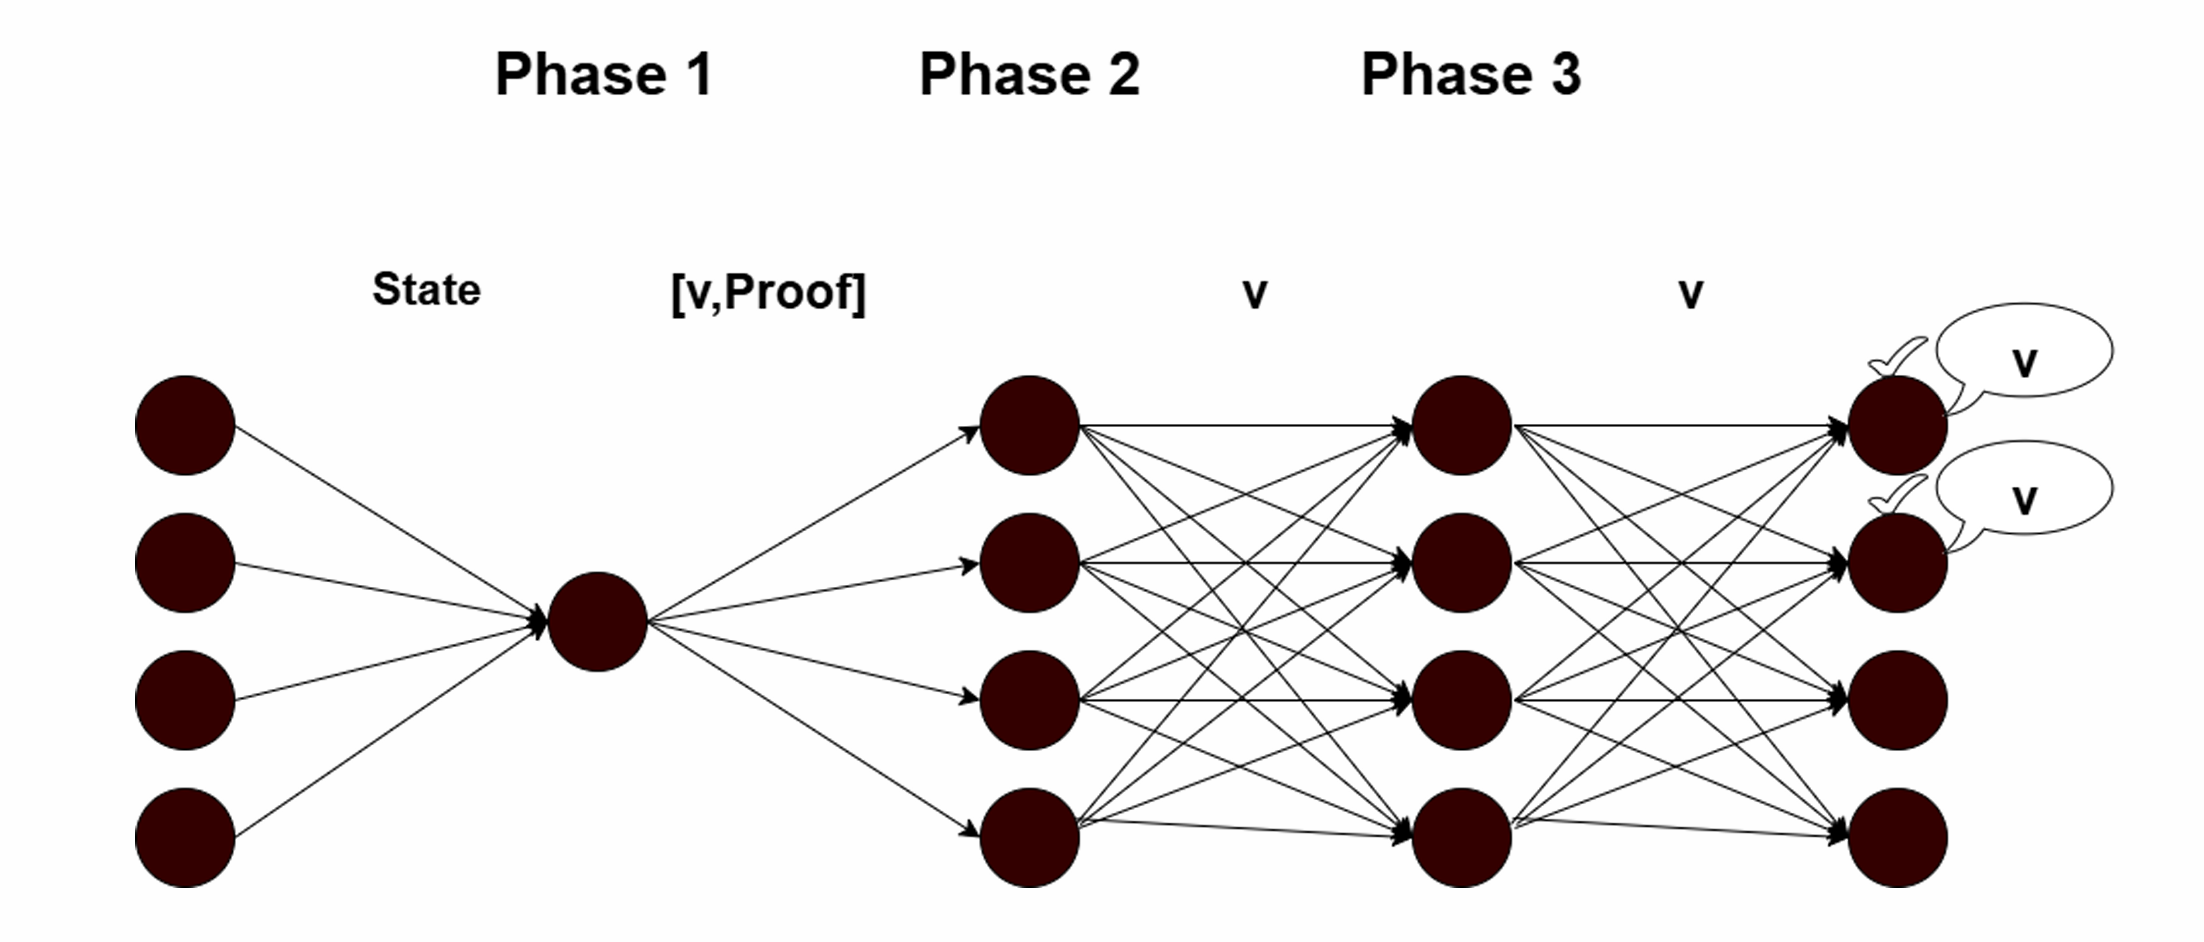
\includegraphics[width=0.8\linewidth]{epog.png}  % Change filename and size as needed
    \caption{Communication flow of the PBFT algorithm as it progresses through its three phases.}
    \label{fig:PBFT}
\end{figure}




We now review the PBFT protocol. First, we introduce the epoch consensus abstraction for the symmetric trust setting that it implements, and then we discuss the specifics of the protocol’s implementation.

\subsubsection{Symmetric Epoch Consensus Specification}
The epoch consensus abstraction is a primitive by which processes agree on a value proposed by the leader of a given epoch. Each epoch has a globally known leader, identified by its epoch timestamp. Since the leader may be faulty, an epoch consensus instance can be aborted, in which case the protocol moves to the next epoch under a new leader. An epoch terminates at a process either by triggering the $\op{Decide}$ event or when a new epoch begins and the $\op{StartEpoch}$ event is triggered.

Module~\ref{modSEP} defines the properties of the Symmetric Epoch Consensus abstraction. These properties closely correspond to those of Weak Byzantine Consensus. The \textit{Weak Validity} property allows decisions on values proposed in earlier epochs. The additional \textit{Lock‑in} property ties together the sequence of epochs, ensuring that once a correct process decides a value in any epoch, no correct process can decide a different value in any later epoch.

Module~\ref{modSEP} omits termination conditions, as they must be adapted to the epoch change abstraction described above. Termination is revisited when we present the APBFT algorithm.




\begin{module*}
	\vbox{
		\small
		\begin{numbertabbing}
			xxxx\=xxxx\=xxxx\=xxxx\=xxxx\=xxxx\=MMMMMMMMMMMMMMMMMMM\=\kill
			\textbf{Module:} \\
			\> Name: SymmetricEpochConsensus, \instance{sep} \\[2ex]
			\textbf{Events:} \\
			\> \textbf{Request}: \(\op{sep.Propose}(v)\): Propose value $v$ for epoch consensus. Executed only by the leader $\ell$. \\
            \>\textbf{Indication}: \(\op{sep.Decide}(v)\): Output the decided value $v$ of epoch consensus. \\
            \\
            \>\textbf{Request}: \(\op{sep.StartEpoch}(\ts,\ell)\): Start a new epoch $\ts$ with leader $\ell$. \\
            \\
            \\

			
			\textbf{Properties:} \\
			\> \textbf{EP1:} \textit{Weak Validity}: If all processes are correct and a process decides $v$ in epoch $\ets$, then $v$\\
            \> was proposed by the leader of some epoch $\ts' \leq \ets$.\\
            \\
            \> \textbf{EP2: } \textit{Agreement}:  No two correct processes decide differently during an epoch.\\
            \\
            \> \textbf{EP3: } \textit{Integrity}: Every correct process decides at most once during an epoch.\\
            \\
            \> \textbf{EP4: } \textit{Lock-in}: If a correct process has decided some value $v$ in an epoch\\
            \> with timestamp $\ts' < \ets$, then no correct process decides a different value in epoch $\ets$.\\
            \\
            
		\end{numbertabbing}
	}
	\caption{Interface and Properties of the Symmetric Epoch Consensus Abstraction}
	\label{modSEP}
\end{module*}

\subsubsection{Algorithm Description}

The PBFT protocol proceeds in three phases, each motivated by the need to guard against Byzantine misbehavior and to ensure that future leaders can reliably detect past support:

\begin{enumerate}
  \item \textbf{Proposal Phase.}  
  The leader of epoch \(\ets\) gathers from a quorum of replicas: 
  \begin{itemize}  
    \item their \emph{write‑sets}, containing all values they have validated in earlier epochs, and  
    \item their persisted state \((\ts, v)\), the most recent epoch and value each replica has recorded.  
  \end{itemize}  
  Inspecting the highest‑timestamped state \((\ts, v)\) allows the leader to respect the lock‑in rule, adopting any previously committed value rather than inventing a new one. The write‑sets serve to certify that the chosen \((\ts, v)\) was genuinely stored by correct replicas and cannot be fabricated by a Byzantine leader. The leader then broadcasts  
  \[
    \msg{\str{decision}}{v,\,\var{proof}}
  \]  
  indicating that evidence for \(v\) accompanies its proposal. The exact construction of \(\var{proof}\) is discussed in the next paragraph.

  \item \textbf{Validation (Write) Phase.}  
  Upon receiving \(\msg{\str{decision}}{v,\var{proof}}\), each replica:  
  \begin{itemize}
    \item Verifies that the leader supplied a valid proof.  
    \item Records \((\ets, v)\) in its local write‑set to persist the intent to decide \(v\). This step prevents future leaders from fabricating a decision that never had quorum support.  
    \item Broadcasts \(\msg{\str{write}}{v}\) to all peers, echoing the proposed value to validate that the leader has sent the same decision value to all replicas.  
  \end{itemize}  
  Once a replica collects a quorum of matching \(\msg{\str{write}}{v}\) messages, it considers \(v\) \emph{validated} and advances to the pre‑commit phase.

  \item \textbf{Pre‑Commit Phase.}  
  To ensure that any subsequent leader can detect that a quorum of replicas was ready to decide \(v\), each replica:  
  \begin{itemize}
    \item Persists the pair \((\ets, v)\) in its local state. This durable storage guarantees that future leaders cannot ignore the fact that \(v\) had sufficient support.  
    \item Broadcasts \(\msg{\str{precommit}}{v}\) to its peers, signaling its final readiness to decide.  
  \end{itemize}  
  When a replica gathers a quorum of identical \(\msg{\str{precommit}}{v}\) messages, it knows that enough correct replicas have durably recorded \((\ets, v)\) and safely triggers  
  \[
    \op{sep.Decide}(v).
  \]
\end{enumerate}
The communication flow and the 3 phase structure of the PBFT algorithm is illustrated in Figure~\ref{fig:PBFT}

\newcommand\halted {\var{halted}\xspace}
\newcommand\proposed {\var{proposed}\xspace}

\newcommand\certify {\var{certify}\xspace}
\newcommand\verify {\var{verify}\xspace}
\newcommand\proposal {\var{proposal}\xspace}

\newcommand \process{\var{process}}
\newcommand \tupvalue{\var{value}}
\newcommand \signature{\var{signature}}
\newcommand \writeset{\var{writeset}}
\newcommand \timestamp{\var{timestamp}}


\paragraph{Safety Mechanism.}

The structure of phase 2 and 3 of the algorithm ensures that the persisted states and write-sets of the replicas contain all the information the leader of an epoch requires to avoid violating the \textit{Lock-In} property. For any given epoch, if a correct process has decided in a previous epoch, then, by the structure of the third phase, a quorum of processes must have persisted that value to their state in that epoch. Therefore, by the quorum intersection property, each quorum of collected states must contain at least one such state testifying to a potential decision on that value. Therefore, in the absence of Byzantine processes, it would thus suffice for the leader to set its decision value to the value of the state with the highest timestamp. This is formalized using the predicate $\op{couldbind}$, which is defined below.

We adopt a fixed naming convention across all predicate definitions: the parameters $\val$ and $\ts$ always denote a value and a timestamp that together represent a state, and $S$ always denotes a set of tuples containing at least the components $(\process,\tupvalue,\timestamp)$. For each process $\process$, the pair $(\tupvalue,\timestamp)$ records its state at the beginning of the epoch. We refer to any such $S$ as a set of states.

In the following predicate definitions, the notation $S_{(\process)}$ denotes the projection of the set of tuples $S$ onto the $\process$ component of the tuples. To make the notation more concise: given a set $A$ consisting of tuples with components $(x,y,z)$, the notation $A_{(x,y)}$ denotes the set $\{(x,y) \mid (x,y,z) \in A\}$. This notation will be used throughout the text.


\begin{numbertabbing}
xxxx\=xxxx\=xxxx\=xxxx\=xxxx\=xxxx\=MMMMMMMMMMMMMMMMMMM\=\kill
$\op{couldbind}(S,\ts,\val) \quad \iff$  \\
\\
\> $S_{(\process)} \in \CQ$ // The processes of $S$ form a quorum \\
\\
\> $\land\, (\val, \ts) \in S_{(\tupvalue,\timestamp)}$ // The state $(\val,\ts)$ is contained in the states of $S$ \\
\\
\> $\land\, \forall \ts' \in S_{(\timestamp)} : \ts' \leq \ts$ // The state $(\val,\ts)$ is the state with the highest timestamp in $S$ \\
\\
\> $\land\, \forall (\val',\ts') \in S_{(\tupvalue,\timestamp)} : \ts' = \ts \implies \val' = \val$ // The state $(\val,\ts)$\\
\>\>is the unique state with maximal timestamp

\end{numbertabbing}
In the presence of Byzantine processes, the $\op{couldbind}$ predicate alone is no longer sufficient to guarantee the \textit{Lock-In} property. After a process has decided on some value $v$, Byzantine processes can attempt to violate the \textit{Lock-In} property by sending a forged state to the leader with a different decision value and a higher timestamp.

To prevent this attack, the leader and replicas only accept a state $(\val, \ts)$ that satisfies $\op{couldbind}$ if there is also evidence that $\val$ was written by a correct process in some epoch $\ts' \geq \ts$. Hence, if correct processes only write decision values that preserve the \textit{Lock-In} property, this attack becomes impossible.

This is where the write-set comes into play: it records which decision values each process has actually written in each epoch. We formalize this verification using the $\op{cert}$ predicate. Intuitively, the $\op{cert}$ predicate checks whether the write-sets of a coreset of processes contain a write of the decision value $\val$ in an epoch during or after epoch $\ts$. By the definition of a coreset, the $\op{cert}$ predicate can only be satisfied if a correct process has indeed written the value as required.

Formally, the predicate takes as input a new type of argument, $W$, called a set of witnesses. $W$ consists of tuples containing at least the components $(\process, \writeset)$, where each $\writeset$ is the write-set of process $\process$ at the start of the epoch. As with the set $S$, whenever we refer to a set $W$ for a predicate, it is assumed to be a set of tuples of this form.

\begin{numbertabbing}
xxxx\=xxxx\=xxxx\=xxxx\=xxxx\=xxxx\=MMMMMMMMMMMMMMMMMMM\=\kill
$\op{cert}(W,\ts,\val) \quad \iff$\\
\\
\> $W_{(\process)} \in \CC$ // The processes of $W$ form a coreset \\
\\
\> $\land \; \forall \ws \in W_{(\writeset)}, \exists \ts' \geq \ts : (\val,\ts') \in \ws $ // The write-sets record \\
\>\> that $\val$ was written in or after epoch $\ts$

\end{numbertabbing}
The predicate $\op{bind}$ combines the $\op{couldbind}$ and $\op{cert}$ predicates to implement the safety mechanism described above.
\begin{numbertabbing}
xxxx\=xxxx\=xxxx\=xxxx\=xxxx\=xxxx\=MMMMMMMMMMMMMMMMMMM\=\kill
$\op{bind}(S,W,\ts,\val) \quad \iff$\\
\\ 
\> $\op{couldbind}(S,\val,\ts)$ // The state $(\val,\ts)$ satisfies $\op{couldbind}$ \\
\\
\> $\land\, \op{cert}(W,\ts,\val)$ // The set of witnesses $W$ certifies the state $(\val,\ts)$ \\
\end{numbertabbing}
To protect against faulty leaders, replicas verify the leader’s work by accepting its decision value only if it provides them with a set of states and witnesses that satisfy the $\op{bind}$ predicate for that value. To prevent the leader from manipulating the collected states, each process signs the state it send to the leader, and replicas only accept states that are presented with correct signatures.

Finally, the leader and replicas need a way to handle the situation where none of the quorums satisfy $\op{bind}$. This situation occurs in particular after the initialization of the system, when every process has the state $(\perp, 0)$.

By disallowing $\perp$ as a decision value, collecting a quorum of initial states proves to the replicas that no correct process has decided in any previous epoch. Therefore, in this scenario, it is safe for the replicas to accept any decision value proposed by the leader without violating the \textit{Lock-In} property. This condition is expressed by the predicate $\op{unbound}$.

\begin{numbertabbing}
xxxx\=xxxx\=xxxx\=xxxx\=xxxx\=xxxx\=MMMMMMMMMMMMMMMMMMM\=\kill
$\op{unbound}(S) \quad \iff$\\
\\
\> $S_{(\process)} \in \CQ$ // The processes of $S$ form a quorum \\
\\
\> $\land\, \forall (\val,\ts) \in S_{(\tupvalue,\timestamp)} : (\val,\ts) = (\perp,0)$ // Every process in $S$ has the initial state 
\end{numbertabbing}
The complete code for the epoch-consensus mechanism of the PBFT algorithm is shown in Algorithms~\ref{alg:PBFT1}--\ref{alg:PBFT3}.
Every message is timestamped with the epoch, to ensure that messages from different epochs cannot interfere.


\begin{algo*}
  \vbox{
  \small
  \begin{numbertabbing}
    xxxx\=xxxx\=xxxx\=xxxx\=xxxx\=xxxx\=MMMMMMMMMMMMMMMMMMM\=\kill
    \textbf{state} \\
    \> \((\val,\ts,\ws) \gets (\perp,0,\{\})\) // Process state \label{}\\
    \> \(\proposal \gets \perp\) // Processes proposal\label{} \\ 
    \> $\ets \gets 0$ // Current epoch \label{} \\
    \> $\ell \gets \perp$ // Leader of the current epoch \label{} \\
    \\
    \> // Phase 1 variables\\
    \> \( \received \gets \{\}\) // Collected states by the leader; stores tuples of the form \label{}\\
\>\>$(\timestamp,\tupvalue,\writeset,\process,\signature)$, where $\timestamp, \tupvalue$ and $\writeset$ is the local state\\
    \>\>of processes $\process$ and $\signature$ is its signature for that state \\
    \\

    \>// Phase 2 variables\\
    \> \(\sent \gets \false\) // Tracks if the process has already sent a WRITE msg \label{}\\
    \> \( \written \gets [\perp]^n\) // Received writes \label{}\\
    \\

    \>// Phase 3 variables\\
    \> \(\decided \gets \false\) // Tracks if the process has decided\label{}\\
    \> \(\wrote \gets \false\) // Tracks if the process has written to its state\label{}\\
    \> \( \accepted
    \gets [\perp]^n\) // Received decides \label{}\\
   \\

    \textbf{upon event} \(\op{StartEpoch}(\var{epoch}, \var{leader})\) \textbf{do}\label{}\\
    \> // Reset the epoch specific state variables \label{}\\
    \> \( \ets \gets \var{epoch}\)\label{}\\
    \> \(\ell \gets \var{leader}\)\label{}\\
    \> \(\received \gets \{\}\) \label{} \\
    \> \(\sent \gets \false\) \label{} \\
    \> \(\written \gets [\perp]^n\)\label{}\\
    \> \(\decided \gets \false\) \label{} \\
    \> \( \wrote \gets \false\)\label{} \\
    \> \( \accepted \gets [\perp]^n\) \label{}\\
    \\
    \> \(\var{prevState} \gets (\val,\ts,\ws)\) \label{}\\
    \> \( \sigma \gets \op{sign}_i(\var{prevState})\) \label{} \\
    \> send message \(\msg{input}{(\var{prevState},\sigma,\ets)}\) to leader $\ell$\label{}\\
    \\
     \textbf{upon event} \(\op{propose}(v)\) \textbf{do} \label{}\\
     \> \( \textbf{if } \proposal = \perp \textbf{then } \proposal \gets v\)\label{}\\
     \>\(\proposed \gets \true\) \label{} \\
    \\
    \textbf{upon} receive a message \( \msg{input}{(\var{prevState},\sigma, \ts')}\) from $p_j$ \textbf{such that} $\ts'=\ets$ \textbf{do}\label{}\\
    \>\textbf{if} \(\op{verify}_j(\var{prevState},\sigma)\) \textbf{then}\label{}\\
    \>\> \(\received \gets \received \cup \{(\var{prevState}^*,p_j,\sigma)\}\)\label{}\\ 
    \\
   \textbf{upon event} \(\proposed \land \exists S,W \subseteq \received, v \neq \perp \ts \in \BN : \op{bind}(v,\ts,S,W)\) \textbf{do} \label{}\\
   \> send message \(\msg{bind}{v,\ts,S,W,\ets} \) to $p_j \in \CP$\label{}\\
   \\
   \textbf{upon event} \(\proposed \land \exists S \subseteq \received : \op{unbound}(S)\) \textbf{do} \label{}\\
   \> send message \(\msg{unbound}{\proposal,S,\ets} \) to $p_j \in \CP$\label{}\\
   \\
   \textbf{upon} receive a message \(\msg{bind}{\val,\ts,S,W,\ts'}\) from $\ell$ \textbf{such that} $\ts'=\ets$ \textbf{do} \label{}\\
   \>\textbf{if} \( \forall (\var{state},p_j,\sigma) \in S \cup W : \op{verify}_j(\var{state},\sigma) \land \op{bind}(\val,\ts,S,W)\) \textbf{then} \label{}\\
   \>\> \textbf{trigger} \( \op{Phase2}(\val,\ets)\)\label{}\\
   \\
    \textbf{upon} receive a message \(\msg{unbound}{\val,S,\ts'}\) from $\ell$ \textbf{such that} $\ts' = \ets$ \textbf{do} \label{}\\
   \>\textbf{if} \( \forall (\var{state},p_j,\sigma) \in S : \op{verify}_j(\var{state},\sigma) \land \op{unbound}(S)\) \textbf{then} \label{}\\
   \>\> \textbf{trigger} \( \op{Phase2}(\val, \ets)\)\label{}\\
   \\
  \end{numbertabbing}
  }
  \caption{PBFT/PAPBFT (Part 1, Decision Phase) (Process $p_i$).}
  \label{alg:PBFT1}
\end{algo*}

\begin{algo*}
  \vbox{
  \small
  \begin{numbertabbing}
    xxxx\=xxxx\=xxxx\=xxxx\=xxxx\=xxxx\=MMMMMMMMMMMMMMMMMMM\=\kill
    
     \textbf{upon event} \(\op{Phase2}(v,\ts')\) \textbf{such that} \( \lnot \written \land \ts' = \ets\) \textbf{do} \label{}\\
     \> \(\written \gets \true\) \label{} \\
     \> \textbf{if} \(\exists \ts' : (\ts', v) \in \ws\) \textbf{then }\label{}\\
    \>\> \(\ws \gets \ws \setminus (\ts', v)\)\label{}\\
    \> \( \ws \gets \ws \cup (\ets, v)\)\label{}\\
    \> send message \( \msg{\str{write}}{v,\ets}\) to all \(p_j \in \CP\)\label{}\\
    \\
    \textbf{upon} receive a message \( \msg{write}{v,\ts'}\) from $p_j$ \textbf{ such that} $\ts' = \ets$ \textbf{do}\label{}\\
    \> \(\written[j] \gets v\)\label{}\\
    \\
    \textbf{upon} \(\exists v \neq perp\) \textbf{such that} \(\{p_j \in \CP \vert \written[j] = v\} \in \CQ\) \textbf{do} \label{} \\
    \> \textbf{trigger} \(\op{Phase3}(v, \ets)\) \label{}
  \end{numbertabbing}
  }
  \caption{PBFT (Part 2, Write/Validation phase) (Process $p_i$).}
  \label{alg:PBFT2}
\end{algo*}

\begin{algo*}
  \vbox{
  \small
  \begin{numbertabbing}
    xxxx\=xxxx\=xxxx\=xxxx\=xxxx\=xxxx\=MMMMMMMMMMMMMMMMMMM\=\kill
    
     \textbf{upon event} \(\op{Phase3}(v,\ts')\) \textbf{such that} $\ts' = \ets$ \textbf{do} \label{}\\
     \> \((\val,\ts) \gets (v,\ets)\) \label{l:write_state} \\
     \> send message \(\msg{precommit}{v,\ets}\) to \(p_j \in \CP\)\label{}\\
    \\
    \textbf{upon} receive a message \( \msg{precommit}{v,\ts'}\) from $p_j$ \textbf{such that} $\ts' = \ets$ \textbf{do}\label{}\\
    \> \(\accepted[j] \gets v\) \label{} \\
    \\
    \textbf{upon} \(\lnot\decided\land \exists v \neq \perp\) \textbf{such that} \(\{p_j \in \CP \vert \accepted[j] = v\} \in \CQ\) \textbf{do} \label{l:e_p_decide} \\
    \> \(\decided \gets \true\)\label{}\\
    \> \textbf{trigger} \(\op{sep.Decide}(v)\) \label{} \\
  \end{numbertabbing}
  }
  \caption{PBFT (Part 3, Pre-Commit Phase) (Process $p_i$).}
  \label{alg:PBFT3}
\end{algo*}

\subsection{PAPBFT: A Hybrid Approach}

In this section, we review an asymmetric PBFT epoch-consensus algorithm proposed by Zanolini~\cite{Zanolini2023}. We discuss the adaptations made to the original PBFT algorithm and highlight the main drawback of this variation. No formal specification of the algorithm’s interface is given, since this algorithm is not the main focus of the section and is very similar to the asymmetric epoch-consensus interface of APBFT, which is presented in the next subsection.

\subsubsection{Algorithm Description}
The usual recipe of replacing quorums, kernels, and core sets with their asymmetric counterparts~\cite{DBLP:journals/dc/AlposCTZ24} fails in phase 1 of the PBFT algorithm. In the first phase, the leader and replicas rely on states from a quorum of processes to deduce the system’s state, in particular to identify whether a process has or has not decided in a previous epoch. In the symmetric setting, all processes share the same set of quorums; hence, each quorum serves as a snapshot of the system that all processes agree upon and accept. However, in the asymmetric setting, every process defines its own set of quorums, and therefore no single quorum exists that serves as a global snapshot of the system for all processes.

 Zanolini works around this issue by operating on the quorum system $\CH$, derived from the tolerated system $\CT$ of the asymmetric quorum system. This resolves the problem, since the tolerated system is again a symmetric quorum system, and therefore its quorums once again serve as a global snapshot shared among the processes.

This change in the algorithm is reflected in a straightforward adjustment of the predicates $\op{couldbind}$, $\op{cert}$, and $\op{unbound}$, where each reference to the quorum system $\CQ$ is replaced by the quorum system $\CH$, and every reference to the coreset system $\CC$ of $\CQ$ is replaced by the coreset system $\CC_{\CH}$ of $\CH$, while all other aspects of the predicates remain unchanged. The redefinition of the affected predicates is given below.

\begin{numbertabbing}
xxxx\=xxxx\=xxxx\=xxxx\=xxxx\=xxxx\=MMMMMMMMMMMMMMMMMMM\=\kill
$\op{cert}(W,\ts,\val) \quad \iff$ \\
\\
\> $W_{(\process)} \in \CC_{\CT}$ // The processes of $W$ form a coreset\\
\\
\> $\land \; \forall \ws \in W_{(\writeset)}, \exists \ts' \geq \ts : (\val,\ts') \in \ws$ // The write-sets record \\
\>\> that $\val$ was written in or after epoch $\ts$

\end{numbertabbing}

\begin{numbertabbing}
xxxx\=xxxx\=xxxx\=xxxx\=xxxx\=xxxx\=MMMMMMMMMMMMMMMMMMM\=\kill
$\op{couldbind}(S,\ts,\val) \quad \iff$ \\
\\
\> $S_{(\process)} \in \CH$ //The processes of $S$ form a quorum\\
\\
\> $\land\, (\val, \ts) \in S_{(\tupvalue,\timestamp)}$ // The state $(\val,\ts)$ is contained in the states of $S$\\
\\
\> $\land\, \forall \ts' \in S_{(\timestamp)} : \ts' \leq \ts$ // The state $(\val,\ts)$ is the state with the highest timestamp in $S$ \\
\\
\> $\land\, \forall (\val',\ts') \in S_{(\tupvalue,\timestamp)} : \ts' = \ts \implies \val' = \val$ // The state $(\val,\ts)$\\
\>\>is the unique state with maximal timestamp
\end{numbertabbing}


\begin{numbertabbing}
xxxx\=xxxx\=xxxx\=xxxx\=xxxx\=xxxx\=MMMMMMMMMMMMMMMMMMM\=\kill
$\op{unbound}(S) \quad \iff$ \\
\\
\> $S_{(\process)} \in \CH$ // The processes of $S$ form a quorum\\
\\
\> $\land\, \forall (\val,\ts) \in S_{(\tupvalue,\timestamp)} : (\val,\ts) = (\perp,0)$ // Every process in $S$ has the initial state

\end{numbertabbing}
Algorithms~\ref{alg:PAPBFT2}~and~\ref{alg:PAPBFT3} show the implementation of phases two and three of the consensus algorithm. They differ from the symmetric algorithm only in that they replace the symmetric quorums with asymmetric ones. The pseudocode for the first phase is not shown as it is identical to that of the symmetric case (Algorithm~\ref{alg:PBFT1}), using the redefined $\op{bind}$ and $\op{unbound}$ predicates.

\begin{algo*}
  \vbox{
  \small
  \begin{numbertabbing}
    xxxx\=xxxx\=xxxx\=xxxx\=xxxx\=xxxx\=MMMMMMMMMMMMMMMMMMM\=\kill
    
     \textbf{upon event} \(\op{Phase2}(v, \ts')\) \textbf{such that} \( \lnot \written \land \ts' = \ets \) \textbf{do} \label{}\\
     \> \(\written \gets \true\) \label{} \\
     \> \textbf{if} \(\exists \ts' : (\ts', v) \in \ws\) \textbf{then }\label{}\\
    \>\> \(\ws \gets \ws \setminus (\ts', v)\)\label{}\\
    \> \( \ws \gets \ws \cup (\ets, v)\)\label{}\\
    \> send message \( \msg{\str{write}}{v, \ets}\) to all \(p_j \in \CP\)\label{}\\
    \\
    \textbf{upon} receive a message \( \msg{write}{v, \ts'}\) from $p_j$ \textbf{such that} $\ts' = \ets$ \textbf{do}\label{}\\
    \> \(\written[j] \gets v\)\label{}\\
    \\
    \textbf{upon} \(\exists v \neq \perp\) \textbf{such that} \(\{p_j \in \CP \vert \written[j] = v\} \in \CQ_i\) \textbf{do} \label{} \\
    \> \textbf{trigger} \(\op{Phase3}(v, \ets)\) \label{}
  \end{numbertabbing}
  }
  \caption{PAPBFT (Part 2, Write/Validation Phase) (Process $p_i$).}
  \label{alg:PAPBFT2}
\end{algo*}

\begin{algo*}
  \vbox{
  \small
  \begin{numbertabbing}
    xxxx\=xxxx\=xxxx\=xxxx\=xxxx\=xxxx\=MMMMMMMMMMMMMMMMMMM\=\kill
    
     \textbf{upon event} \(\op{Phase3}(v, \ts')\) \textbf{such that } $\ts' = \ets$  \textbf{do} \label{l:p3_start}\\
     \> \((\val,\ts) \gets (v,\ets)\) \label{} \\
     \> send message \(\msg{precommit}{v, \ets}\) to \(p_j \in \CP\)\label{}\\
    \\
    \textbf{upon} receive a message \( \msg{precommit}{v, \ts'}\) from $p_j$ \textbf{such that} $\ts' = \ets$ \textbf{do}\label{}\\
    \> \(\accepted[j] \gets v\) \label{} \\
    \\
    \textbf{upon} \(\lnot\decided\land \exists v \neq \perp\) \textbf{such that} \(\{p_j \in \CP \vert \accepted[j] = v\} \in \CQ_i\) \textbf{do} \label{l:dec_con} \\
    \> \(\decided \gets \true\)\label{}\\
    \> \textbf{trigger} \(\op{aep.Decide}(v)\) \label{} \\
  \end{numbertabbing}
  }
  \caption{PAPBFT (Part 3, Pre-Commit Phase) (Process $p_i$).}
  \label{alg:PAPBFT3}
\end{algo*}

\subsubsection{Drawback}
This implementation has one major drawback. From a theoretical standpoint, it is a rather unsatisfactory solution to the issue encountered in the first phase when considering asymmetric quorum systems. The algorithm does not provide a true solution to the lack of a global view shared by the processes but instead circumvents the issue by relying once again on a symmetric quorum system. This approach offers no insight into how to address this dilemma within the asymmetric setting itself.

\subsection{Introducing APBFT}

\begin{figure}[htbp]
    \centering
    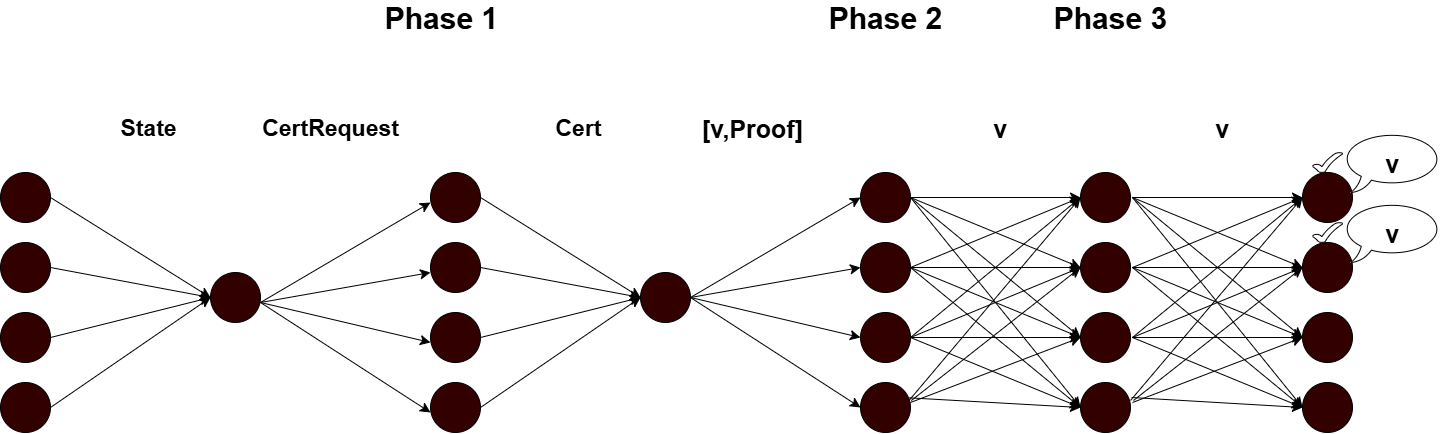
\includegraphics[width=0.8\linewidth]{ep_overview2.drawio.png}  % Change filename and size as needed
    \caption{Communication flow of the APBFT algorithm as it progresses through its three phases. In contrast to the PBFT algorithm, the first phase includes an additional round of communication, in which the leader broadcasts certification requests and the replicas holding a certificate send back a response.}
    \label{fig:APBFT}
\end{figure}

In this section, we introduce the APBFT algorithm, an asymmetric version of the PBFT algorithm that does not rely on the tolerated system. First, we discuss the adaptation of the epoch consensus interface to the asymmetric setting. Next, we describe the adaptations made to PAPBFT to derive the APBFT algorithm, and finally, we prove its correctness.

\subsubsection{Asymmetric Epoch Consensus Specification}

We review the changes made to the epoch consensus interface (shown in Module~\ref{modEP2}) to adapt it to the asymmetric setting. The first four core properties of the epoch consensus abstraction remain semantically the same as in the symmetric setting. However, the guarantees of \textit{Agreement} and \textit{Lock-In} have been restricted to guild members.

The epoch consensus interface specifies two termination conditions. The first, called \textit{Termination}, ensures that when a guild member is the leader of an epoch and the replicas give them sufficient time to fulfill their role, every guild member reaches consensus in that epoch. The second condition, called \textit{One for All}, is a termination guarantee that ensures all guild members in an epoch eventually terminate if at least one other guild member has already decided.

This additional termination condition is required to handle cases where faulty leaders attempt to sabotage system liveness by allowing some guild members to terminate while blocking the progress of others. The \textit{One for All} property prevents this from happening.

\begin{module*}
	\vbox{
		\small
		\begin{numbertabbing}
			xxxx\=xxxx\=xxxx\=xxxx\=xxxx\=xxxx\=MMMMMMMMMMMMMMMMMMM\=\kill
			\textbf{Module:} \\
			\> Name: AsymmetricEpochConsensus, \instance{aep}\\[2ex]
			\textbf{Events:} \\
            \> \textbf{Setup}: \( \op{aep.StartEpoch}(\ets, \ell)\): Progresses epoch consensus to epoch $\ets$\\
            \> with leader $\ell$.\\
            \\
			\> \textbf{Request}: \(\op{aep.Propose}(v)\): Proposes value $v$ for epoch consensus. \\
            \\
            \>\textbf{Indication}: \(\op{aep.Decide}(v)\): Output a decide value $v$ of epoch consensus. \\
            \\

			
			\textbf{Properties:} \\
			\> \textbf{EP1:} \textit{Weak Validity}: If all processes are correct and a process decides $v$ in epoch $\ets$, then $v$\\
            \> was proposed by the leader of some epoch $\ets' \leq \ets$.\\
            \\
            \> \textbf{EP2: } \textit{Agreement}: No two wise processes decide differently in an epoch.\\
            \\
            \> \textbf{EP3: } \textit{Integrity}: Every correct process decides at most once in each epoch.\\
            \\
            \> \textbf{EP4: } \textit{Lock-in}:  If a wise processes has decided some value $v$ in an epoch\\
            \> with timestamp $\ts' < \ts$, then no wise process decides a value different from $v$ in epoch $\ts$.\\
            \\
              \> \textbf{EP5: } \textit{Termination}:  If the leader $\ell$ of some epoch $\ets$ is a guild member, has proposed a value, \\
              \> and all guild members are simultaneously in epoch $\ets$ for a fixed time period,\\
              \>then every guild member decides in epoch $\ets$.\\
            \\
            \> \textbf{EP6: }\textit{One for All}: In every execution with a guild, When a guild member decides in some epoch $\ets$,\\
            \>and all guild members are simultaneously in epoch $\ets$ for a fixed amount of time,\\
            \>then every guild member decides in epoch $\ets$.
            \\
            
		\end{numbertabbing}
	}
	\caption{Interface and Properties of the Asymmetric Epoch Consensus Abstraction}
	\label{modEP2}
\end{module*}


\subsubsection{Algorithm Description}

As mentioned in the previous section, the main difficulty in reformulating the PBFT algorithm lies in how the leader and replicas share a global view of the system via a quorum. This shared view does not exist in the asymmetric setting. Recall what the replicas and the leader try to achieve in the first phase of the algorithm. The job of the leader is to identify a decision value that it can prove to a sufficient number of replicas does not violate the \textit{Lock-In} property, based on the local states of the replicas. The job of the replicas is to verify that proof and proceed to phase 2 of the algorithm only with decision values that respect \textit{Lock-In}.

The key to circumventing the issue of no shared global quorum to rely on is for the leader to collect, for each process, one of its personal quorums to provide it with a personalized proof that the decision value is safe to accept.

In the symmetric setting, the $\op{bind}$ predicate was used to identify decision values that respect \textit{Lock-In}.
The justification for why the $\op{bind}$ predicate preserves \textit{Lock-In} generalizes,for guild members, to the asymmetric setting when swapping symmetric quorums with asymmetric ones.

Below, the redefinition of the $\op{bind}$ and $\op{unbound}$ predicates is given. We defer the redefinition of the $\op{cert}$ predicate to the end of this section, since the certification mechanism needs to be adapted due to weaker guarantees of the epoch change primitive in the asymmetric setting. However, the asymmetric $\op{cert}$ predicate preserves its properties for guild members and serves the same purpose as it does in the symmetric setting.

The predicates additionally take a process identifier as input to index the individual quorum systems. The parameters of the predicates remain unchanged; only the structure of the set of witnesses $W$ differs, which will be discussed when presenting the redefinition of $\op{cert}$.

\begin{numbertabbing}
xxxx\=xxxx\=xxxx\=xxxx\=xxxx\=xxxx\=MMMMMMMMMMMMMMMMMMM\=\kill
$\op{bind}_i(S,W,\val,\ts) \quad \iff$ \\
\\
\> $\op{couldbind}_i(S,\val,\ts)$ // The state $(\val,\ts)$ satisfies $\op{couldbind}_i$\\
\\
\> $\land\, \op{cert}_i(W,\ts,\val)$ // The set of witnesses $W$ certifies the state $(\val,\ts)$

\end{numbertabbing}

\begin{numbertabbing}
xxxx\=xxxx\=xxxx\=xxxx\=xxxx\=xxxx\=MMMMMMMMMMMMMMMMMMM\=\kill
$\op{couldbind}_i(S,\val,\ts) \quad \iff$ \\
\\
\> $S_{(\process)} \in \CQ_i$ // The processes of $S$ form a quorum for process $p_i$\\
\\
\> $\land\, (\val, \ts) \in S_{(\tupvalue,\timestamp)}$ // The state $(\val,\ts)$ is contained in the states of $S$\\
\\
\> $\land\, \forall \ts' \in S_{(\timestamp)} : \ts' \leq \ts$ // The state $(\val,\ts)$ is the state with the highest timestamp in $S$\\
\\
\> $\land\,  \forall (\val',\ts) \in S_{(\tupvalue,\timestamp)} :  \val' = \val$ // The state $(\val,\ts)$ \\
\>\> is the unique state with maximal timestamp 

\end{numbertabbing} 
This adapted $\op{bind}$ predicate behaves identically as in the symmetric case for guild members. In particular, after a guild member has decided on some value $v$, for every guild member $p_i$, $\op{bind}_i$ can only be satisfied by the decision value $v$. However, the converse is not true: $\op{bind}$ being satisfied does not guarantee that a guild member has previously decided. Recall that in the symmetric case, the $\op{unbound}$ predicate proved to a replica that no correct process had yet decided. This concept generalizes naturally to the asymmetric setting.

\begin{numbertabbing}
xxxx\=xxxx\=xxxx\=xxxx\=xxxx\=xxxx\=MMMMMMMMMMMMMMMMMMM\=\kill
$\op{unbound}_i(S) \quad \iff$ \\
\\
\> $S_{(\process)} \in \CQ_i$ // The processes of $S$ form a quorum for process $p_i$\\
\\
\> $\land\, \forall (\val,\ts) \in S_{(\tupvalue,\timestamp)} : (\val,\ts) = (\perp,0)$ // Every process in $S$ has the initial state

\end{numbertabbing}
The key idea in the construction of the APBFT algorithm is the introduction of an additional predicate that proves to a guild member that no guild member has yet decided. By combining the ideas of the $\op{unbound}$ and $\op{bind}$ predicates, a replica can conclude that a decision value is safe to accept when confronted with a set of states and witnesses $S$ and $K$ that bind to a state $(\val,\ts)$, and, in addition, a set of witnesses $K'$ that certify they have written some different value $\val' \neq \val$ in an epoch with timestamp $\ts' > \ts$.

\begin{numbertabbing}
xxxx\=xxxx\=xxxx\=xxxx\=xxxx\=xxxx\=MMMMMMMMMMMMMMMMMMM\=\kill
$\op{debind}_i(S,W,W',\val,\ts) \quad \iff$ \\
\\
\> $\exists \val'\neq \val, \ts' < \ts :  \op{bind}_i(S,W,\val',\ts')$ // Predicate $\op{bind}_i$ is satisfied\\
\>\>for a value $\val' \neq \val$ with a timestamp $\ts'<\ts$\\
\\
\> $\land\,  \op{cert}_i(W',\val,\ts)$ // The set of witnesses $W'$ certifies $(\val,\ts)$

\end{numbertabbing}
This third predicate increases the number of decision values a replica can accept, thereby facilitating the leader's task of identifying a decision value that a sufficient number of replicas can accept.

The final decision rule, by which a replica can identify safe decision values, is expressed by the predicate $V$ (for Verify). It combines the three predicates: $\op{bind}$, $\op{unbound}$, and $\op{debind}$.

\begin{numbertabbing}
xxxx\=xxxx\=xxxx\=xxxx\=xxxx\=xxxx\=MMMMMMMMMMMMMMMMMMM\=\kill
$V_i(S,W,W',\val) \quad \iff$\\
\\
\> $\op{unbound}_i(S)$ // Predicate $\op{unbound}_i$ is satisfied\\
\\
\> $\lor\,  \exists \ts \in \BN : \op{bind}_i(S,W,\val,\ts)$ // Predicate $\op{bind}_i$ is satisfied\\
\\
\> $\lor\,\exists \ts  \in \BN : \op{debind}_i(S,W,W',\val,\ts)$ // Predicate $\op{debind}_i$ is satisfied
\end{numbertabbing} 
The predicate $V$ has the desirable property that, in every execution of the algorithm, it can be satisfied with the same decision value for every guild member. Thus, for the leader of an epoch to choose a suitable decision value, it must collect states until it detects a quorum for itself of processes that satisfy $V$ with the same decision value. If the leader is a guild member, such a quorum is guaranteed to exist, and this quorum suffices to drive the epoch to consensus.

The decision rule of the leader is formalized as the predicate $C_i(Q,S,W,\val)$, standing for Collect. The input parameter $Q$ is a set of processes forming a quorum for the leader $p_i$. The sets $S$ and $W$ are the sets of states and witnesses, respectively. They carry all the required information for satisfying the $V$ predicate for every process in the quorum $Q$ for the same decision value $\val$.

\begin{numbertabbing}
xxxx\=xxxx\=xxxx\=xxxx\=xxxx\=xxxx\=MMMMMMMMMMMMMMMMMMM\=\kill
$C_i(Q,S,W,\val) \quad \iff$ \\
\\
\> $Q \in \CQ_i$ // The set of processes $Q$ is a quorum for the leader\\
\\
\> $\land\,   \forall p_j \in Q , \exists S' \subseteq S, \; W', W'' \subseteq W, \ts \in \BN : V_j(S',W',W''\val,\ts)$\\
\>\> // For every process in $Q$ the process can verify $\val$
\end{numbertabbing} 
Since the leader can only determine a decision value for a quorum for itself, processes also write a value in the second phase of the algorithm when they receive a kernel for themselves of write messages from their peers. This ensures that eventually all wise processes write a value, even if they never complete the first phase.

One final change must be made to the original PBFT algorithm due to the weaker properties of the Asymmetric Epoch Change abstraction. Namely, in the asymmetric setting, the proposed epoch change mechanism, \textit{Eventual Entry}, only ensures progression through the epochs for guild members. This means that wise and naive processes may get stuck in some epoch, even though the system did not, and will not, reach consensus in that epoch. This is problematic because the $V$ predicate relies on kernels of processes that certify a state with their write sets.

When a wise process decides on $v$ in some epoch $\ets$, the structure of the second and third phases of the algorithm ensures that, for every guild member, a kernel for itself of correct processes exists that certifies the state $(v, \ets)$. However, since this kernel need not consist exclusively of guild members, some processes certifying the state may get stuck in lower epochs. As a result, the leader may never collect their states and thus never observe the kernel, potentially jeopardizing the liveness of the algorithm.

To address this issue, instead of processes sending their write-sets to the leader at the start of the first phase of the algorithm, they only send their local state $(\val, \ts)$. The leader then uses the $\op{couldbind}$ predicate to identify states that require certification. The leader subsequently broadcasts a request to the replicas, asking them to certify the requested state. Once a process is able to certify the requested state, it sends a signed acknowledgment back to the leader, attesting that it can indeed certify the requested state.
This additional communication step is illustrated in Figure~\ref{fig:APBFT}
\newcommand \witnesses {\var{witnesses}\xspace}
\newcommand \witnessset {\var{witnessSet}\xspace}


The leader stores this information in a set of tuples called $\witnesses$, of the form $(\tupvalue, \timestamp, \witnessset)$, where $\witnessset$ is a set of tuples of the form $(\process, \signature)$, each consisting of a process and a signature. These tuples represent processes that have messaged the leader, stating that they can certify the state $(\tupvalue, \timestamp)$, with the signature preventing the leader from forging certificates. The $\op{cert}_i$ predicate is redefined to operate on this new data structure; it checks whether a set of witnesses $W$ contains a kernel for process $p_i$ that certify $\val$ for some timestamp $\ts'\geq \ts$.

In the symmetric setting, we relied on coresets for the certification process. In the APBFT algorithm, we instead rely on kernels, since kernels provide the same key guarantee as coresets in the symmetric setting, namely, that they contain at least one correct process, which is required to justify the definition of the $\op{cert}$ predicate.

However, in the asymmetric setting, coresets provide weaker guarantees than kernels. Coresets for guild members still preserve the guarantee that they contain at least one correct process. This guarantee is weaker, however, because this correct process might be naive, making its testimony that it has written a value unreliable, as naive processes are not protected from writing decision values that violate the \textit{Lock-In} property. Kernels for guild members, on the other hand, provide the stronger guarantee of containing at least one other guild member, which mimics the mechanism of coresets in the symmetric setting.  

\newcommand \decisionvalue {\var{decisionvalue}\xspace}

\begin{numbertabbing}
xxxx\=xxxx\=xxxx\=xxxx\=xxxx\=xxxx\=MMMMMMMMMMMMMMMMMMM\=\kill
$\op{cert}_i(W,\ts,\val) \quad \iff$\\
\\
\> $\exists K \in \CK_i , \forall p_j \in K, \exists (\val,\ts',w)\in W : \ts' \geq \ts \land p_j \in w_{(\process)}$\\
\>\> // $W$ contains a kernel of certificates for $(\ts,\val)$
\end{numbertabbing} 
The final code for the first and second phases is shown in Algorithms~\ref{alg:APBFTState}--\ref{alg:APBFT2}. Phase 3 remains unchanged as in Algorithm~\ref{alg:PAPBFT3}.

\begin{algo*}
  \vbox{
  \small
  \begin{numbertabbing}
    xxxx\=xxxx\=xxxx\=xxxx\=xxxx\=xxxx\=MMMMMMMMMMMMMMMMMMM\=\kill
    \textbf{implements}\\
    \> AsymmetricEpochConsensus, \instance{aep}\\
    \\
        \textbf{state} \\
    \> \((\val,\ts,\ws) \gets (\perp,0,\{\})\) // Process state \label{}\\
    \> \(\proposal \gets \perp\) // Processes proposal\label{} \\ 
    \> $\ets \gets 0$ // Current epoch \label{} \\
    \> $\ell \gets \perp$ // Leader of the current epoch \label{} \\
    \\
    \> // Phase 1 variables\\
    \> \(\decisionvalue \gets \perp\) // Leaders identified decision value \label{} \\
      \> \( \received \gets \{\}\) // Collected states by the leader; stores tuples of the form \label{}\\
\>\>$(\timestamp,\tupvalue,\process,\signature)$, where $\timestamp$ and $ \tupvalue$ is the local state\\
    \>\>of processes $\process$ and $\signature$ is its signature for that state \\
    \\

    \>// Phase 2 variables\\
    \> \(\sent \gets \false\) // Tracks if the process has already sent a WRITE msg \label{}\\
    \> \( \written \gets [\perp]^n\) // Received writes \label{}\\
    \\

    \>// Phase 3 variables\\
    \> \(\decided \gets \false\) // Tracks if the process has decided\label{}\\
    \> \(\wrote \gets \false\) // Tracks if the process has written to its state\label{}\\
    \> \( \accepted
    \gets [\perp]^n\) // Received decides \label{}\\
   \\
   \> // certification datastructures\\
    \> \(\witnesses \gets \{\}\) // Contains tuples of the form $(\tupvalue,\timestamp,\var{certificates})$ where $\var{certificates}$\label{}\\
    \>\>is a set of tuples of the form $(\process,\signature)$ of processes\\
    \>\>that certify the state $(\tupvalue,\timestamp)$ and there signatures $\signature$\\
    \> \(\certify \gets \{\}\) // Set of tuples of the form $(\tupvalue,\timestamp,\process)$\label{}\\
    \>\>storing the state pairs $(\tupvalue,\timestamp)$ that leader $\process$ needs a certificate for\\
\\
    \textbf{upon event} \(\op{StartEpoch}(\var{epoch}, \var{leader})\) \textbf{do}\label{l:e_p_s_e}\\
    \> // Reset the epoch specific state variables \label{}\\
    \> \( \ets \gets \var{epoch}\)\label{}\\
    \> \(\ell \gets \var{leader}\)\label{}\\
    \> \(\received \gets \{\}\) \label{} \\
    \> \(\sent \gets \false\) \label{} \\
    \> \(\written \gets [\perp]^n\)\label{}\\
    \> \(\decided \gets \false\) \label{l:dec_g_false} \\
    \> \( \wrote \gets \false\)\label{} \\
    \> \( \accepted \gets [\perp]^n\) \label{}\\
    \> \(\decisionvalue \gets \perp\) \label{} \\
    \\
    \> \(\var{prevState} \gets (\val,\ts)\) \label{}\\
    \> \( \sigma \gets \op{sign}_i(\var{prevState})\) \label{l:g_sig_p_1} \\
    \> send message \(\msg{input}{(\var{prevState},\sigma,\ets)}\) to leader $\ell$\label{}\\
    \\

  \end{numbertabbing}
  }
  \caption{State Variables and Epoch Initialization of APBFT (Process $p_i$).}
  \label{alg:APBFTState}
\end{algo*}

\begin{algo*}
  \vbox{
  \small
  \begin{numbertabbing}
    xxxx\=xxxx\=xxxx\=xxxx\=xxxx\=xxxx\=MMMMMMMMMMMMMMMMMMM\=\kill

     \textbf{upon event} \(\op{propose}(v)\) \textbf{do} \label{}\\
     \> \( \textbf{if } \proposal = \perp \textbf{then } \proposal \gets v\)\label{}\\
     \>\(\proposed \gets \true\) \label{} \\
    \\
    \textbf{upon} receive a message \( \msg{input}{(\var{prevState},\sigma, \ts')}\) from $p_j$ \textbf{such that} $\ts'=\ets$ \textbf{do}\label{}\\
    \>\textbf{if} \( \op{verify}_j(\var{prevState},\sigma)\) \textbf{then}\label{l:leader_very_states}\\
    \>\> \(\received \gets \received \cup \{(\var{prevState}^*,p_j,\sigma)\}\)\label{}\\ 
    \\
   \textbf{upon } \(
\exists  p_j \in \CP, \; v \neq \perp, \; \ts \in \mathbb{N}, S \subseteq \received  : \op{couldbind}_j(S,v,\ts)\land (v,\ts,\cdot) \not  \in \witnesses\) \textbf{do}\label{l:l_couldbind}\\
\> \(\witnesses \gets \witnesses \cup \{(v,\ts,\{\})\}\)\label{l:w_init}\\
\> send message \(\msg{certify}{v,\ts} \text{ to all } p_j \in \CP\)\label{}\\
\\
\textbf{upon} receive a message \(\msg{certify}{v, \ts}\) from $p_j$ \textbf{do} \label{} \\
\> \textbf{if} \(\exists \ts' \leq \ts : (v,\ts') \in \ws\) \textbf{then} \label{} \\
\>\> \(\sigma \gets \op{sign}_i((v,\ts))\) \label{l:cert_sign_1}\\ 
\>\> send message \(\msg{verified}{(v,\ts),\sigma}\) to $p_j$ \label{} \\
\> \textbf{else} \label{}\\
\>\> \(\certify \gets \certify \cup \{(v,\ts,p_j)\}\)\label{} \\
\\

\textbf{upon} receive message $\msg{verified}{(v,\ts),\sigma}$ from $p_j$ \textbf{do} \label{} \\
\> \textbf{if} \( \op{verify}_j((v,\ts),\sigma) \land \exists (v,\ts,w) \in \witnesses\) \textbf{then}\label{l:check_wit_lead} \\
\>\> \( w \gets w \cup (p_j,\sigma)\)\label{}\\
\\
\textbf{upon} $\proposal \neq \perp \land \; \exists v \neq \perp ,\; Q \in \CQ_i: C_i(Q,\received,\witnesses,v)$ \textbf{do} \hfill // Only leader \(\ell\) \label{l:leaderbind}\\

    \> \textbf{if} $\forall p_j \in Q, \exists S_j \subseteq \received : \op{unbound}_j(S_j)$ \textbf{then} \label{l:all_unbound}\\
    \>\> $\decisionvalue \gets \proposal$\label{}\\ 
    \> \textbf{else} \label{} \\
    \>\> $\decisionvalue \gets v$\label{l:set_val}\\
    \\

  \textbf{upon} \( \decisionvalue \neq \perp , \; \exists p_j\in\CP, \; S \subseteq \received, \; W,W' \subseteq \witnesses : V_j(S,W, W',\decisionvalue)\) \textbf{do}\label{l:v_sat}\\
    \> send message \(\msg{\str{bind}}{S, W, W', \decisionvalue, \ets}\) to $p_j$\label{l:send_bind}\\
    \\

   \textbf{upon} receive a message \(\msg{bind}{S,W,W', \decisionvalue,\ts'}\) from $\ell$ \textbf{such that} $\ts'=\ets$ \textbf{do} \label{l:fol_bind}\\
   \>\textbf{if} \( \forall (\var{state},p_j,\sigma) \in S  : \op{verify}_j(\var{state},\sigma)\)  \label{l:replicas_very_states}\\ 
   \>\>\>\( \land \forall (v, \ts, w) \in W \cup W' , (p_j, \sigma) \in w : \op{verify}_j((v,\ts), \sigma)\)\label{l:check_witness_rep}\\
   \>\>\> \(\land V_i(S,W,W',\decisionvalue)\) \textbf{then} \label{l:v_sat_replicas}\\
   \>\> \textbf{trigger} \( \op{write}(\decisionvalue,\ets)\)\label{l:p1_write}\\
   
  \end{numbertabbing}
  }
  \caption{APBFT (part 1, Decision Phase) (Process $p_i$).}
  \label{alg:APBFT1}
\end{algo*}

\begin{algo*}
  \vbox{
  \small
  \begin{numbertabbing}
    xxxx\=xxxx\=xxxx\=xxxx\=xxxx\=xxxx\=MMMMMMMMMMMMMMMMMMM\=\kill
    
     \textbf{upon event} \(\op{write}(v,\ts')\) \textbf{such that} \( \lnot \wrote \land \ts' = \ets\) \textbf{do} \label{l:write_event}\\
     \> \(\wrote \gets \true\) \label{} \\
     \> \textbf{if} \(\exists \ts' : (\ts', v) \in \ws\) \textbf{then }\label{}\\
    \>\> \(\ws \gets \ws \setminus (\ts', v)\)\label{}\\
    \> \( \ws \gets \ws \cup (\ets, v)\)\label{l:add_ws}\\
    \> send message \( \msg{\str{write}}{v,\ets}\) to all \(p_j \in \CP\)\label{}\\
     \> \textbf{if } \(\exists \ts \leq \ets, \; p_j \in \CP : (v,\ts, p_j) \in \certify\) \textbf{then }\label{l:g_if1}\\
     \>\> \(\sigma \gets \op{sign}_i((v,\ts))\)\label{l:g_sigma}\\
    \> \> send message \(\msg{\str{verified}}{(v, \ts), \sigma}\) to \(q\)\label{}\\
    \> \> \(\certify \gets \certify \setminus \{(v,\ts,p_j)\}\)\label{}\\
    \\
    \textbf{upon } \(\exists v \neq \perp\) \textbf{such that} \(\{p_j \in \CP \vert \written[j] = v\} \in \CK_i\) \textbf{do} \label{l:kernel_write} \\
    \> \textbf{trigger} \(\op{write}(v,\ets)\)\label{}\\
    \\
    \textbf{upon} receive a message \( \msg{write}{v,\ts'}\) from $p_j$ \textbf{ such that} $\ts' = \ets$ \textbf{do}\label{}\\
    \> \(\written[j] \gets v\)\label{}\\
    \\
    \textbf{upon} \(\exists v \neq \perp\) \textbf{such that} \(\{p_j \in \CP \vert \written[j] = v\} \in \CQ_i\) \textbf{do} \label{l:quorum_con_p2} \\
    \> \textbf{trigger} \(\op{Phase3}(v, \ets)\) \label{}
  \end{numbertabbing}
  }
  \caption{APBFT (part 2, Write/Validation Phase) (Process $p_i$).}
  \label{alg:APBFT2}
\end{algo*}



\subsubsection{Algorithm Correctness}

In this section, we prove the correctness of the APBFT algorithm. We begin by formalizing the properties of the predicates discussed in the previous section and conclude by showing that APBFT implements the Asymmetric Epoch Consensus abstraction.

Throughout the following proofs, we make repeated use of the following terminology:
In the execution of the epoch consensus algorithm, the first $\op{startEpoch}$ event marks the beginning of the first epoch. The period between two $\op{startEpoch}$ events defines the execution of an epoch, where the first event is referred to as the start of the epoch and the second as the end. Each epoch is identified by the value of the variable $\ets$.

A process $p_i$ is said to satisfy a predicate if, during the execution of the protocol, the predicate evaluates to $\true$ at process $p_i$ at some time $t$.

The following lemma establishes the desired property of the $\op{cert}$ predicate.

\begin{lemma}
\label{lem:certkernel}
In every execution with a guild, if a correct process $p_j$ satisfies the predicate $\op{cert}_i(W,v,\ts)$ in epoch $\ets$ at time $t$, where $p_i \in \CG{\text{max}}$, then there exists another process $p_g \in \CG_{\text{max}}$ that wrote $v$ at time $t_g < t$ in some epoch $\ts_g \geq \ts$.
\end{lemma}
\begin{proof}
    A correct processes $p_j$ only satisfies $\op{cert}_i$ when it is the leader of an epoch (on lines~\ref{l:v_sat} and~\ref{l:leaderbind}), while satisfying predicates $C_j$ and $V_i$. Also $p_i$ satisfies $\op{cert}_i$ when satisfying $V_i$ on line~\ref{l:v_sat_replicas}. In all three cases, $\op{cert}_i$ is invoked on a set $W$ containing tuples $(v',\ts',w)$, where $w$ contains process-signature pairs $(p_h,\sigma)$. In all three cases, on lines~\ref{l:check_wit_lead}~and~\ref{l:check_witness_rep}, before satisfying $\op{cert}_i$, the processes first check that the signature $\sigma$ was generated by process $p_h$ for the state $(v',\ts')$ by verifying that $\op{verify}_h((v',\ts'),\sigma)$ is true for all tuples in $W$.
    However, a correct processes $p_h$ only generates this signature on lines~\ref{l:cert_sign_1}~and~\ref{l:g_sigma}, after checking that its write set contains a pair $(v',\ts'')$ with $\ts' \geq \ts''$. Since $p_h$ only adds tuple $(v',\ts'')$ to its write set on line~\ref{l:add_ws} when writing $v'$ in epoch $\ts''$,
    this establishes that every correct process in $w$ has, in fact written $v'$ in some epoch $\ts'' \geq \ts'$ at some time $t' < t$ as desired. 
    
    Furthermore, by the definition of the predicate $\op{cert}_i$, $W$ satisfies it only when it contains a kernel $K \in \CK_i$ for $p_i$. 
    By Lemma~\ref{lem:g_kernel}, there is a guild member $p_g \in \CG_{\text{max}}$ contained in $K$.
    Also, by the definition of $\op{cert}_i$ there is a tuple $(v,\ts_g,w_g)$ in $W$ such that $p_g \in w_g$ and $\ts_g \geq \ts$. As argued above, this establishes that $p_g$ wrote $v$ in epoch $\ts_g$ at some time $t_g < t$, as desired.   
\end{proof}

\begin{lemma}
\label{lem:wellformed}
If a correct process $p_h$ satisfies the predicate $\op{unbound}_i(S)$ or $\op{couldbind}_i(S,\cdot,\cdot)$ in some epoch $\ets$, for a correct process $p_i$, then for all $(v, \ts, p_j) \in S_{(\tupvalue, \timestamp, \process)}$, the pair $(v, \ts)$ is the local state of $p_j$ at the end of epoch $\ets - 1$.
\end{lemma}
\begin{proof}
    The predicate $\op{unbound}_i$ or $\op{couldbind}_i$ is only satisfied on lines~\ref{l:l_couldbind}, \ref{l:leaderbind}, \ref{l:v_sat}~and~\ref{l:v_sat_replicas}, either by the leader of epoch $\ets$ or by $p_i$ itself if its correct. In both cases, the set $S$ consists of tuples $(v,\ts,p_j,\sigma)$ and the processes ensure that the state $(v,\ts)$ indeed originates from processes $p_j$ by performing the check $\op{verify}_j((v,\ts), \sigma)$ on lines~\ref{l:leader_very_states}~and~\ref{l:replicas_very_states}, before satisfying the predicates. Since a correct $p_j$ only generates this signature at the start of the first phase(line~\ref{l:g_sig_p_1}) this establishes that $(v',\ts')$ is the state of $p_j$ at the end of epoch $\ets-1$.
\end{proof}

The next lemma establishes the property, that for guild members $p_i$ the predicate $V_i$ can only be satisfied with decision values that do not violate the \textit{Lock-In} property, starting off with two helper lemmas.

\begin{lemma}
    \label{lem:stateSync}
    If in some epoch $\ets$ a wise process $p_i$ writes $(v,\ets)$ to its local state, then no other wise process writes $(v',\ets)$ to its local state for $v' \neq v$ in that epoch.
\end{lemma}
\begin{proof}
    Process $p_i$ only writes $(v,\ets)$ to its local state after receiving $\str{write}$ messages for $v$ from a quorum $Q$ for itself (lines~\ref{l:quorum_con_p2}~and~\ref{l:write_state}). Assume that there is another wise process that writes $(v',\ets)$ to its local state with $v \neq v'$, which it would only do after receiving $\str{write}$ messages for $v'$ from a quorum $Q'$ for itself (line~\ref{l:quorum_con_p2}). By the quorum intersection property, there is a correct process in the intersection of $Q$ and $Q'$, implying that it has sent a $\str{write}$ message for both $v$ and $v'$, contradicting the fact that a correct process only sends a single $\str{write}$ message in each epoch. This is ensured by the fact that the $\op{write}$ event is guarded by a $\lnot \wrote$ condition, which is set to $\true$ before sending the write message on line~\ref{l:write_event}. The $\wrote$ variable is only reset to $\false$ when triggering the $\op{startEpoch}$ event, which also increments the $\ets$ variable(line~\ref{l:e_p_s_e}).
\end{proof}

\begin{lemma}
    \label{lem:unsatUnbound}
    After a wise process $p_j$ decides $v \neq \perp$ in some epoch $\ets$, no correct process satisfies $\op{unbound}_i$ for any wise process $p_i$.
\end{lemma}
\begin{proof}
    By the structure of the third phase of the algorithm, process $p_j$ only decides $v$ after receiving $\str{precommit}$ messages for $v$ from a quorum $Q_j \in \CQ_j$ for itself (line~\ref{l:e_p_decide}). Observe that a correct process only sends a $\str{precommit}$ message after writing $(v,\ets)$ to its local state (line~\ref{l:write_state}). 
    
    Now assume that there is a correct process $p_k$ that satisfies $\op{unbound}_i(S)$ in some epoch $\ets' > \ets$. By the quorum intersection property, $S_{(\process)}$ and $Q_j$ intersect in a correct process $p_h$. Let $(v_h,\ets_h,p_h,\cdot) \in S$ be the tuple in $S$ corresponding to process $p_h$. Since $\op{unbound}_h(S)$ is satisfied, $v_h = \perp$.
    By Lemma~\ref{lem:wellformed}, $(v_h,\ets_h)$ is the local state of $p_h$ at the end of epoch $\ets' -1 $. Let $t$ be the time at which process $p_h$ writes $(v,\ets)$ to its local state in epoch $\ets$. Since $\ets'-1 \geq \ets$ this means that processes $p_h$ ends epoch $\ets'-1$ at time $t' > t$. Observe that no correct process ever writes $\perp$ to its local state, which implies that $v_h \neq \perp$, a contradiction. 
\end{proof}




\begin{lemma}
    \label{lem:Vsafety}
    In every execution with a guild, if a correct process satisfies the predicate $V_i(S,W,W',v)$ in some epoch $\ets$ and $p_i \in \CG_{\text{max}}$, then no wise process has decided a value $v' \neq v$ in any epoch $\ts' < \ets$.   
\end{lemma}
\begin{proof}
    
    For the sake of contradiction assume that $V_i(S,W,W',v)$ is satisfied, yet a wise process $p_w$ has decided $v' \neq v$ in some epoch $\ts' < \ets$. Process $p_w$ only decides after receiving $\str{precommit}$ messages for $v'$ from a quorum $Q_w$ for itself (line~\ref{l:e_p_decide}). Each correct process in $Q_w$ only send a $\str{precommit}$ message for $v'$ after setting its local state to $(v',ts')$ (line~\ref{l:write_state}).
    
    Since by Lemma~\ref{lem:unsatUnbound}, $\op{unbound}_i$ cannot be satisfied, $\op{bind}_i$ or $\op{debind}_i$ must be satisfied for $V_i$ to hold.
    
    Observe that correct processes only write strictly increasing timestamps to their local state, since the sequence of epochs is strictly increasing. By definition, a timestamp $\ts''$ can only satisfy $\op{couldbind}(S,v',\ts'')$ if $\ts''$ is the maximal timestamp in $S$. Therefore, by the quorum intersection property of $Q_{w}$ and $S_{(\process)}$ and the above observation applied to $Q_w$, it follows that $\ts''$ can only satisfy $\op{couldbind}_i$, if $\ts'' \geq \ts'$. Hence $\op{bind}_i$ can only be satisfied by a timestamp $\geq \ts'$. Therefore, by definition, $\op{debind}_i$ can also only be satisfied by a timestamp $> \ts'$. 
    
    In fact, like $\op{debind}_i(S,W,W',v,\ts'')$, $\op{bind}_i(S,W,v,\ts'')$ can also only be satisfied by a $\ts''$, that is strictly larger than $\ts'$. This also follows from the quorum intersection property of $S_{(\process)}$ and $Q_w$, and the unique maximal state condition of the  $\op{couldbind}_i$ predicate. In the case where $\ts'' = \ts'$ if, for sake of contradiction, $\op{bind}(S,W,v,\ts')$ is satisfied, then $(v,\ts')$ is the unique maximal state in $S$. By quorum intersection of $S_{(\process)}$ and $Q_w$, $S$ contains the state information of a correct process $p_c \in Q_w$. Let $(v_c,\ts_c,p_c,\cdot) \in S$ be the tuple in $S$ associated with process $p_c$. Since correct processes write strictly increasing timestamps to their local state, $\ts_c  \geq \ts'$. Therefore, $\ts_c$ is the maximal timestamp in $S$, and it follows that $\ts_c = \ts'$ and $v_c = v$. However, $p_c$ had state $(v',\ts')$, and since $p_c$ only writes strictly increasing timestamps to its state, it follows that $v'=v$, a contradiction. This establishes that $\op{bind}_i$ can only be satisfied with a timestamp $> \ts'$ for value $v$.
    
    By definition for $\op{bind}_i(S,W,v,\ts'')$ or $\op{debind}_i(S,W,W',v,\ts'')$ to be satisfied with a timestamp $\ts'' > \ts'$, it must hold that $\op{cert}_i(W,v,\ts'')$ or $\op{cert}_i(W',v,\ts'')$ is satisfied. By Lemma~\ref{lem:certkernel}, a guild member must exist that writes $v$ during or after epoch $\ts''$. Let $p_g \in \CG_{\text{max}}$ be the first guild member that writes $v$ in some epoch $\ets_g$ such that $\ets_g > \ts'$. Denote the time of this event by $t_{g_1}$. Since $p_g$ is the first guild member to write $v$ in epoch $\ets_g$, by Lemma~\ref{lem:g_kernel}, its write cannot have occurred by satisfying the kernel condition on line~\ref{l:kernel_write}. Therefore $p_g$ must have written the value after returning it from the first phase (line~\ref{l:p1_write}). This means that $p_g$ satisfied $V_g(S_g,W_g,W'_g,v)$ for some $S_g$, $W_g$ and $W'_g$. Denote by $t_{g_2} < t_{g_1}$ the time at which this occurs. Since $\ets_g > ts'$, by the same reasoning as above, $\op{unbound}_g(S_g)$ is unsatisfiable and $\op{bind}_g(S_g,W_g,v,ts_g)$ or $\op{debind}_g(S_g,W_g,W'_g,v,ts_g)$ can only be satisfied by a timestamp $\ts_g > \ts'$. This, as argued above, implies that another guild member $p_{g'} \in \CG_{\text{max}}$ wrote $v$ in some epoch with timestamp $\ets_{g'} > \ts'$, at some time $t_{g'}$ where clearly $t_{g'} < t_{g_2} < t_{g_1}$, contradicting the minimality of $p_g$. 
\end{proof}
Finally we establish the liveness property of the $C_i$ predicate showing that it is always satisfiable when the leader is a guild member, again starting off with a helper lemma.

\begin{lemma}
    \label{lem:verifyState}
    when a wise process $p_w$ writes $(\val,\ets)$ to its local state at time $t$, then at any time $t' \geq t$, for every other wise process $p_{w'}$ a kernel $K \in \CK_{w'}$ for $p_{w'}$ of correct processes exist that can verify the state $(\val, \ets)$. Meaning that every process in $K$ has an entry $(\val,\ts)$ in its write set, such that $\ts \geq \ets$. 
\end{lemma}
\begin{proof}
    $p_w$ only writes $(\val,\ets)$ to its local state after receiving a $\str{write}$ message for $\val$ from a quorum $Q_w$ for itself in epoch $\ets$. By lemma~\ref{lem:wise_kernel} $Q_w$ contains a kernel $K_{w'}$ for $p_{w'}$ of correct processes for every wise process $p_{w'}$. Since every correct process only sends a $\str{write}$ message for $\val$ in epoch $\ets$ after adding $(\val,\ets)$ to its write set. Furthermore a correct processes never removes a value from its write set, it only replaces a tuple $(\val,\ets)$  by another tuple $(\val,\ets')$, with $\ets' > \ets$, when writing $\val$ in a later epoch $\ets'$. Hence  every process in $K_{w'}$ can always verify $(\val,\ets)$ after time $t$.
\end{proof}

\begin{lemma}
    \label{lem:C_liv}
    After $\var{GST}$, in every execution with a guild, if the leader $p_\ell \in \CG_{\text{max}}$ of some epoch $\ets$ is a guild member and all guild members start epoch $\ets$, then $p_{\ell}$ satisfies $C_{\ell}$ within $3 \Delta$ time steps, assuming $p_{\ell}$ does not move to a new epoch in the meantime.
\end{lemma}
\begin{proof}
    After the last guild member starts epoch $\ets$ at time $t$, he sends his state to $p_{\ell}$ (line~\ref{l:e_p_s_e}), which arrives no later than at time $t+\Delta$. Let $Q_\ell$ denote the leader’s guild quorum, and let $Q_g$ denote the guild quorum for each guild member $p_g \in Q_{\ell}$. Once $p_{\ell}$ receives the state from the last guild member, the leader can satisfy $\op{couldbind}_g$ or $\op{unbound}_g$ for every guild member $p_g$.
    
    Let $S^g$ be the states of the processes in $Q_g$. More precisely, define $S^g := \{(v,\ts,p_j,\sigma) \in \received \mid p_j \in Q_g  \}$. If every state in $S^g$ is the initialization state, i.e., $\forall (v,\ts) \in S^g_{(\tupvalue,\timestamp)} : (v,\ts) = (\perp,0)$, then $\op{unbound}_g(S^g)$ is satisfied. Observe that for all $ \ts >0$, we have $(\perp, \ts) \not \in S^g_{(\tupvalue,\timestamp)}$, since correct processes never write $\perp$ to their local state. Hence if $\op{unbound}_g(S^g)$ is not satisfied, it follows that there exists a state $ (v,\ts) \in S^g_{(\tupvalue,\timestamp)}$ such that $ v \neq \perp$. Moreover, since correct processes only write strictly increasing timestamps to their local state, it follows that $\ts > 0$. Furthermore, since every process in $Q_g$ is wise, it follows from Lemma~\ref{lem:stateSync} that states in $S^g$ that share the same timestamp have the same decision value. More formally, this means that $\forall (v,\ts), (v',\ts') \in S^g_{(\tupvalue,\timestamp)} : \ts = \ts' \implies v = v'$.
    Hence, some state $(v_g^{\text{max}},\ts_g^{\text{max}})$ with a maximal timestamp in $S^g$ clearly satisfies $\op{couldbind}_g(S^g,v_g^{\text{max}},\ts_g^{\text{max}})$.
    
    This establishes that at time $t+\Delta$, the leader can either satisfy $\op{unbound}_g$, or has satisfied $\op{couldbind}_g$ and broadcast a verification request (line~\ref{l:l_couldbind}) for the state $(v_g ^{\text{max}},\ts_g^{\text{max}})$ if he has not done so previously. Therefore, by Lemma~\ref{lem:verifyState}, the leader receives, for every $p_g$, a kernel for $p_g$ of certificates for each state $(v_g^{\text{max}},\ts_g^{\text{max}})$ after $2\Delta$ time steps.
    More formally, Lemma~\ref{lem:verifyState} establishes that for every guild member $p_g' \in Q_{\ell}$ and every maximal state $(v_g^{\text{max}},\ts_g^{\text{max}})$ of some guild member $p_g \in Q_{\ell}$, the singleton subset $K := \{(v^{\text{max}}_g,\ts^{\text{max}}_g,w) \in \witnesses\}$ satisfies $\op{cert}_{g'}(K,v^{\text{max}}_g,\ts^{\text{max}}_g)$.
    
    This shows that the leader satisfies $C_{\ell}(Q_{\ell},\received,\witnesses, v^{\text{max}})$ (line~\ref{l:leaderbind}), where $(v^{\text{max}}, \ts^{\text{max}})$ is the state with the maximal timestamp among the states $(v_g^{\text{max}}, \ts_g^{\text{max}})$ for the processes $p_g$ in the leader’s guild quorum $Q_{\ell}$. To see this, recall that as stated above, for every process in $p_g \in Q_{\ell}$, the leader satisfies either $\op{unbound}_g$ or $\op{couldbind}_g$. In the first case $V_g$ is satisfied. In the second case, if $\ts_g^{\text{max}} = \ts^{\text{max}}$, then again by Lemma~\ref{lem:stateSync}, it follows that $v^{\text{max}} = v_g^{\text{max}}$, and hence $\op{bind}_g(S^g,W_g,v^{\text{max}},\ts^{\text{max}})$ is satisfied, where $W_g \subseteq \witnesses$ contains the kernel for $p_g$ of witnesses for the state $(v^{\text{max}},\ts^{\text{max}})$. Thus, $V_g$ is satisfied. Recall that the existence of $W_g$ has been established above by showing that $\witnesses$ contains a kernel for $p_g$ of witnesses for every state $v_g^{\text{max}},\ts_g^{\text{max}}$ and every guild member $p_g$.
    
    In the scenario where $\ts_g^{\text{max}} < \ts^{\text{max}}$, then $\op{debind}_g(S^g,W_g,W'_g,v^{\text{max}},\ts^{\text{max}})$ is satisfied, where $W_g \subseteq \witnesses$ contains the kernel for $p_g$ of witnesses that certify $(v_g^{\text{max}},\ts_g^{\text{max}})$ and $W'_g \subseteq \witnesses$ contains the kernel for $p_g$ of witnesses that certify $(v^{\text{max}},\ts^{\text{max}})$.\\
    Hence every process $p_g \in Q_{\ell}$ satisfies $V_g$ for value $v^{\text{max}}$, and therefore $p_{\ell}$ satisfies $C_{\ell}(Q_{\ell},\received,\witnesses)$ at most after $3\Delta$ time steps after the last guild member started the epoch.
\end{proof}

We now show that APBFT implements the Asymmetric Epoch Consensus interface.

\begin{theorem}
\label{t:ep_correctness}
    The APBFT algorithm implements the Asymmetric Epoch Consensus interface
\end{theorem}
\begin{proof}
    We first show \textit{Weak Validity}. First, Observe that all processes are guild members, since all processes are correct. A process decides $v$ in epoch $\ets$ only after receiving $\str{precommit}$ messages for $v$ from a quorum for itself (line~\ref{l:dec_con}). Furthermore, a process only sends a $\str{precommit}$ message for $v$ after receiving $\str{write}$ messages for $v$ from a quorum for itself in epoch $\ets$ (line~\ref{l:quorum_con_p2}). Let $p_g$ be the first process to send a $\str{write}$ message for $v$ in some epoch $\ets'$. By the minimality of $p_g$, this can only occur after the process has returned $v$ from the first phase of the algorithm (line~\ref{l:p1_write}). The leader $\ell'$ of epoch $\ets'$ sends $v$ to $p_g$ (line~\ref{l:v_sat}) only after satisfying the $C_{\ell'}$ predicate (line~\ref{l:leaderbind}), which requires collecting states and certificates such that a quorum $Q_{\ell'}$ for the leader satisfies the $\op{bind}$, $\op{debind}$, or $\op{unbound}$ predicate for value $v$.
    Observe that $\op{cert}_j(\cdot,v,\cdot)$ is unsatisfiable for all processes $p_j \in Q_{\ell'}$, since otherwise, by Lemma~\ref{lem:certkernel}, this would contradict the minimality of $p_g$. This implies, by definition, that for all processes $p_j \in Q_{\ell'}$, both $\op{bind}_j(\cdot,\cdot,v,\cdot)$ and $\op{debind}_j(\cdot,\cdot,\cdot,v,\cdot)$ are unsatisfiable. Therefore, all processes in $Q_{\ell'}$ must satisfy the $\op{unbound}$ predicate for $C_{\ell'}(Q_{\ell'},\var{states},\var{witnesses},v)$ to be satisfied. Thus, the leader satisfies the condition on line~\ref{l:all_unbound}, and therefore $v$ is the proposal of $\ell'$, establishing \textit{Weak Validity}.
    
    
    The \textit{Agreement} property follows directly from Lemma~\ref{lem:stateSync}, since correct processes only send $\str{precommit}$ messages for values that they have written to their local state in a given epoch (line~\ref{l:p3_start}).
    
    \textit{Integrity} is ensured by the $\lnot \decided$ guard on the event that triggers $\op{Decide}$ (line~\ref{l:dec_con}). The guard is set to $\true$ before deciding, and is only reset once a new epoch starts (line~\ref{l:dec_g_false}).
    
    To show \textit{Lock-In:} Assume a process $p_i$ has decided on value $v$ in some epoch $\ets$. For the sake of contradiction, assume that a process $p_j$ decides on a value $v' \neq v$ in some epoch $\ets' > \ets$. It follows that $p_j$ has received a $\str{precommit}$ message for $v'$ from a quorum $Q$ for itself (line~\ref{l:dec_con}). $Q$ contains a guild member $p_k$, who has received a quorum for itself of $\str{write}$ messages for $v'$ (line~\ref{l:quorum_con_p2}), which itself includes a guild member. Let $p_h$ be the first guild member to write $v$ in epoch $\ets'$. By the minimality of $p_h$ and Lemma~\ref{lem:g_kernel}, $p_h$ cannot have written $v'$ after receiving a kernel for itself of $\str{write}$ messages for $v'$ (line~\ref{l:kernel_write}), and must therefore have returned $v'$ from the first phase of the algorithm (line~\ref{l:p1_write}). This implies that $p_h$ satisfied predicate $V_k(\cdot,\cdot,\cdot, v')$ (line~\ref{l:v_sat_replicas}). Lemma~\ref{lem:Vsafety} then directly contradicts the assumption that $p_i$ decided $v$ in epoch $\ets < \ets'$. 
    
    
    
    To show \textit{Termination}, recall that Lemma~\ref{lem:C_liv} establishes that a quorum $Q \in \CQ_\ell$ for $\ell$ returns a decision value $v$ from the first phase of the algorithm after at most $\var{GST}+3\Delta$ time steps. After returning from the first phase (line~\ref{l:p1_write}), these processes write $v$, sending a $\str{write}$ message to all peers (line~\ref{l:write_event}). By Lemma~\ref{lem:wise_kernel}, this implies that every wise process receives a $\str{write}$ message for $v$ from a kernel for itself. Hence, after at most $\var{GST}+4\Delta$ time steps, every wise process satisfies the kernel condition on line~\ref{l:kernel_write} and also broadcasts a $\str{write}$ message for $v$ to its peers. Therefore, by the availability condition, every wise process receives $\str{write}$ messages for $v$ from a quorum for itself after at most $\var{GST}+5\Delta$ time steps. Hence, every wise process sends a $\str{precommit}$ message for $v$ (line~\ref{l:quorum_con_p2}), and subsequently receives $\str{precommit}$ messages from a quorum for itself after at most $\var{GST}+6\Delta$ time steps, and decides $v$ (line~\ref{l:dec_con}).
    
    Finally, to show \textit{One for All}, if a wise process decides value $v$ in epoch $\ets$, it must have received $\str{precommit}$ messages from a quorum $Q$ for itself line \ref{l:dec_con}). $Q$ must contain at least one wise process, which only sends a $\str{precommit}$ message for $v$ after receiving $\str{write}$ messages for $v$ from a quorum $Q'$ for itself line~\ref{l:quorum_con_p2}). By Lemma~\ref{lem:wise_kernel}, $Q'$ contains a kernel for every wise process. Hence, every wise process must eventually receive a kernel for itself of $\str{write}$ messages for $v$, and therefore must eventually write $v$ itself line~\ref{l:kernel_write}). As argued for the \textit{Termination} condition, this ensures that every wise process eventually receives a quorum for itself of $\str{write}$ messages for $v$, and hence eventually receives a quorum for itself of $\str{precommit}$ messages for $v$, and thus eventually decides $v$.
\end{proof}


\section{Leader-Driven Consensus Algorithm}
In this final section, we present the glue code that combines the Asymmetric Epoch Change and Asymmetric Epoch Consensus abstractions into a single consensus algorithm implementing Asymmetric Weak Byzantine Consensus.

The Leader-Driven Consensus Algorithm is shown in Algorithm~\ref{alg:l_d_c}. Upon receiving a $\op{aec.StartEpoch}$ event from the epoch change abstraction, the algorithm relays this information to the epoch consensus abstraction by triggering its corresponding $\op{aep.StartEpoch}$ event. Additionally, a timeout is started. The timeout duration is set to a constant multiple of the epoch number, ensuring that the process increases its wait time with each successive epoch.

If the timer expires, the process suspects the leader to be faulty and issues a $\op{aec.Complain}$ event to the epoch change abstraction.
When a value is proposed, it is directly forwarded to the epoch consensus instance. Upon receiving a $\op{aep.Decide}$ event from the epoch consensus instance, the timeout is canceled. If the process has not yet made a decision, it decides on the received value. 
\newcommand \newts{\var{newts}}
\newcommand \newl{\var{new}\ell}

\begin{algo*}
  \vbox{
  \small
  \begin{numbertabbing}
    xxxx\=xxxx\=xxxx\=xxxx\=xxxx\=xxxx\=MMMMMMMMMMMMMMMMMMM\=\kill
    \textbf{implements}\\
    \> AsymmetricWeakByzantineConsensus, \instance{awc}  \\
    \textbf{uses } \\
    \> AsymmetricEpochChange, \instance{aec} \\
    \> AsymmetricEpochConsensus, \instance{aep} \\
    \textbf{state} \\
    \> \( \decided \gets \false \) \label{l:d_init}\\
    \> \( (\ets, \ell) \gets (0, \perp) \) \label{}\\
    \\
    \textbf{upon event} \(\op{awc.Propose}(v)\) \textbf{do} \label{l:wc_prop_event}\\
    \> \( \op{aep.Propose}(v) \) \label{}\\
    \\
    \textbf{upon event}  \( \op{aec.StartEpoch}( \newts, \newl)\) \textbf{such that} $\newts > \ets$ \textbf{do} \label{}\\
    \> \( (\ets, \ell) \gets (\newts, \newl) \) \label{}\\
    \> \textbf{trigger} \( \op{aep.StartEpoch}(\newts, \newl) \) \label{}\\
    \> \( \op{StartTimer}((\newts+1)\cdot\Delta)\) \label{}\\
    \\
    \textbf{upon event} \( \op{aep.Decide} (v) \)  \textbf{do} \label{l:wc_decide_event}\\
    \> $\op{CancelTimer}()$\label{}\\
    \> \textbf{if} \( \lnot\decided \) \textbf{then} \label{l:if_d}\\
    \> \> \( \decided \gets \true \); \label{l:d_true}\\
    \> \> \textbf{trigger} \(\op{awc.Decide}(v) \); \label{}\\
    \\
    
    \textbf{upon event} \( \op{Timeout}\) \textbf{do}\label{}\\
    \> \textbf{trigger} \( \op{aec.Complain}(\ets)\) \label{} \\
  \end{numbertabbing}
  }
  \caption{Leader-Driven Consensus Algorithm (Process $p_i$). }
  \label{alg:l_d_c}
\end{algo*}

\begin{theorem}
    \label{th:ldc_correctness} The Leader-Driven Consensus Algorithm implements Weak Consensus.
\end{theorem}
\begin{proof}
The \textit{Weak Validity} property follows directly from the \textit{Weak Validity} property of the Asymmetric Epoch Consensus abstraction. Assume all processes are correct, and that process $p_i$ decides on a decision value $v$. Process $p_i$ decides only after an $\op{aep.Decide}(v)$ event occurs (line~\ref{l:wc_decide_event}). The \textit{Weak Validity} property of Asymmetric Epoch Consensus ensures that $v$ was $\op{aep.Proposed}$ by some correct process $p_j \in \CP$. However $p_j$ only  $\op{aep.Proposes}$ $v$ immediately after $v$ has been $\op{awc.Propsed}$ by $p_i$ (line~\ref{l:wc_prop_event}), thereby establishing the validity property.

Concerning \textit{Integrity}, observe that before deciding, a process sets its $\decided$ guard to $\true$ (line~\ref{l:d_true}) and only decides when $\lnot \decided$ holds (line~\ref{l:if_d}). Since $\decided$ is only set to $\false$ upon initialization (line~\ref{l:d_init}) \textit{Integrity} is ensured.

To show \textit{Agreement}, assume that some wise process $p_i$ decides $v$, and another wise process $p_j$ decides $v'$. Both processes can only decide after an $\op{aep.Decide}$ event occurs (line \ref{l:wc_decide_event}).
Hence, the \textit{Agreement} and \textit{Lock-In} properties of Asymmetric Epoch Consensus ensure that $v=v'$. The \textit{Agreement} property applies when both processes decide in the same epoch of the epoch consensus instance, and the  \textit{Lock-In} applies when they decide in different epochs.

Finally we show the \textit{Termination} property.
For the sake of contradiction, assume that some guild member $p_g \in \CG_{\text{max}}$ never decides. There are two cases to consider. Either $p_g$ starts an infinite sequence of epochs, or $p_g$ remains in some epoch indefinitely. In the first case, by the \textit{Eventual Entry} property, $p_g$ can only remain indefinitely in an epoch $\ets$  if all guild members remain in the same epoch indefinitely. Therefore, the \textit{Eventual Progression} property of Asymmetric Epoch Change implies that no kernel for all processes ever complains in epoch $\ets$. Since, by Lemma~\ref{lem:glob_kern}, the maximal guild $\CG_{\text{max}}$ contains a kernel for all processes, it follows that some guild member $p_k$ never complains in epoch $\ets$. However, a correct process always complains in an epoch it has started unless it decides in that epoch. Therefore, by the \textit{One for All} property of Asymmetric Epoch Consensus, every guild member decides in epoch $\ets$. In particular $p_g$ decides in epoch $\ets$, a contradiction.

Now consider the latter case, where $p_g$ starts an infinite number of epochs. By the \textit{Eventual Entry} property, this implies that every guild member starts an infinite number of epochs. Since the guild members complain in increasing time intervals, the precondition of the \textit{Unbounded Leadership} property of Asymmetric Epoch Change is satisfied. Combined with the \textit{Uniform Leadership} property, this implies that for any duration $d$ there is some epoch $\ets_d$, such that all guild members are simultaneously in epoch $\ets_d$ for at least that duration and the leader of $\ets_d$ is a guild member. Hence it follows that the guild members are simultaneously in an epoch $\ets$ that satisfies the precondition of the \textit{Termination} property of the epoch consensus abstraction. Therefore, all guild members decide in epoch $\ets$, a contradiction.

\end{proof}

\chapter{Experimental Evaluation}

In this chapter we discuss the experimental evaluation of the PAPBFT algorithm \cite{Zanolini2023} and the Asymmetric Randomized Consensus algorithm \cite{DBLP:journals/jacm/MostefaouiMR15}.

\paragraph{Benchmarking Parameters.}
We empirically investigate the scalability and impact of faulty processes on the running time of the two algorithms. All experiments are performed on three quorum systems consisting of 5, 6, and 7 processes. These quorum systems are taken directly from the example systems provided in the paper by Alpos et al.~\cite{DBLP:journals/dc/AlposCTZ24}, illustrated in Examples 1, 2, and 4. We restrict our analysis to this small collection of quorum systems, since constructing asymmetric quorum systems is a non-trivial task with no known general procedure. Moreover, the benchmark is not suitable for large quorum systems.

To assess scalability, we measure the performance of the algorithms as the number of processes in the quorum system increases.

To evaluate the impact of faulty processes, we compare the algorithms' performance under failure-free conditions to their performance when the maximum allowable number of processes fail. The maximum number of failures is determined by determining the smallest guild in the system while allowing all other processes to fail. Failed nodes are modeled as non-responsive processes that do not reply to messages from their peers. Byzantine nodes are simulated solely as crash faults, since modeling more complex malicious behavior would complicate the benchmarking process without any anticipated impact on the performance of the algorithms compared to crash faults. Verifying this hypothesis is left as future work.

\paragraph{Benchmark Metric.}
The performance of the algorithm is measured using the \textbf{quorum response time} of the quorum system.
To perform this measurement, a dedicated process referred to as the client is introduced. The client is responsible for initiating and observing the execution of the consensus algorithm. The measurement begins when the client sends a start message to all processes in the quorum system that participate in the consensus algorithm, along with a value for them to propose.

Each replica executes the consensus protocol independently. When a replica completes the protocol and reaches a decision, it sends a decide message with the decided value back to the client. The client collects these responses and terminates the measurement once it has received decision messages from any quorum in the asymmetric quorum system.

More formally, for a given quorum system, the client stops the measurement once: 
\[
\exists p_i \in \CP, Q \in \CQ_i : \text{the client has received a decide message from all processes in } Q.
\]

This duration is referred to as the \textbf{quorum response time} of the consensus algorithm. The measuring procedure is illustrated in Figure~\ref{fig:qrt}.

\begin{figure}[htbp]
    \centering
    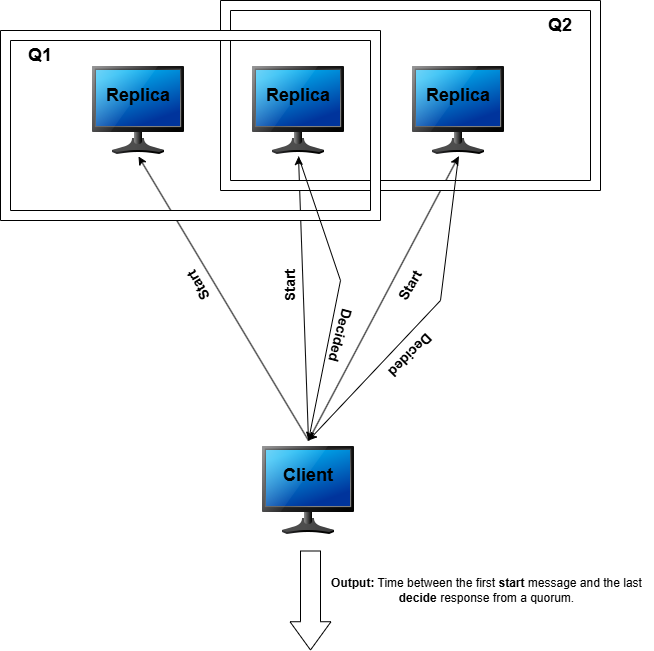
\includegraphics[width=0.8\linewidth]{responseTime.drawio.png}  % Change filename and size as needed
    \caption{Client/Replicas architecture for measuring the \textbf{quorum response time}. The client starts the measurement by sending a start message to all the replicas. The replicas run the consensus algorithm and respond back to the client once they have decided. As soon as the client is informed of some quorum deciding, the measurement is terminated. In the illustration quorum $Q_2$ has decided}
    \label{fig:qrt}
\end{figure}

\paragraph{Hardware Setup.}

All experiments were conducted on a single computer with an AMD Ryzen 7 5800X processor. The network was implemented by communicating locally using the loopback interface (i.e., 127.0.0.1). 


\paragraph{Repetition of Measurements.}
To increase the stability of the measurements, each experiment was repeated 50 times, and the results report the average metric. Furthermore, in each repetition, the identifiers of the processes in the asymmetric quorum system were shuffled to average out the influence of process labeling on the measurement. This labeling has a particularly strong effect on the leader-driven PAPBFT consensus algorithm, where it determines the sequence in which processes are elected as leaders of the epoch consensus instances.

We settled on this number of repetitions because, given the observed standard deviation of the measurements, we believe it is sufficient to obtain a reliable estimate of the true underlying mean.

\paragraph{Asymmetric Common Coin Implementation.} As mentioned in Chapter~\ref{c:async_con}, the common coin of the Asymmetric Randomized Consensus algorithm has not been implemented. To make the algorithm operational, the common coin was substituted with a local random bit generator. To ensure the \textit{Matching} property of the Asymmetric Common Coin abstraction (Module~\ref{modACC}), each random bit generator was initialized with the same seed. This implementation, however, violates the \textit{Unpredictability} property of the abstraction. Nevertheless, this violation does not affect the correctness of the algorithm in the experiment, since the emulated Byzantine processes only crash and therefore do not exploit it.  

\paragraph{Scalability and Performance Comparison.}

Figures~\ref{pic:vary_num_cor} and~\ref{pic:vary_num_fault} show the response times of the two algorithms as the number of processes in the asymmetric quorum system increases and their structures change. Figure~\ref{pic:vary_num_cor} presents results for executions in which all processes are correct, while Figure~\ref{pic:vary_num_fault} shows the scenario where the maximal number of processes fail. A direct comparison of the execution times under both conditions is further summarized in Table~\ref{tab:combined}.

Figure~\ref{pic:vary_num_cor} demonstrates that when all processes are correct, PAPBFT exhibits good scalability. There is no clear upward trend in the quorum response time as the system size increases. In contrast, Asymmetric Randomized Consensus shows poor scalability: as the number of processes increases, the response time increases steadily. The algorithm requires on average 1.75 times longer on 7 than on 5 processes. Moreover, in this failure-free scenario, PAPBFT clearly outperforms Asymmetric Randomized Consensus, with the margin steadily increasing as the number of processes increases. On 5 processes, PAPBFT runs on average 1.35 times faster than Asymmetric Randomized Consensus. On 7 processes, the performance gap significantly increases, with PAPBFT executing 2.66 times faster than Asymmetric Randomized Consensuss on average.

However, this picture changes dramatically in the presence of faults, as illustrated in Figure~\ref{pic:vary_num_fault}. In this scenario, the Asymmetric Randomized Consensus algorithm significantly outperforms PAPBFT, executing between 1.5 and 1.9 times faster than PAPBFT on average.

Table~\ref{tab:combined} offers insight into this performance shift. The performance of the Asymmetric Randomized Consensus algorithm is barely affected by the presence of faulty processes; it remains nearly constant across both conditions. In contrast, the performance of the PAPBFT algorithm degrades substantially when faulty processes are introduced. This behavior is a direct consequence of the Leader-Driven Consensus Paradigm: agreement can only be reached during an epoch led by a correct leader. If the leaders of the first
$k$ epochs are faulty, then, by design, the system spends at least $\Delta \cdot (1+2+...+k) = \Delta \cdot (\frac{k\cdot(k+1)}{2})$ time steps making no progress. Consequently, the choice of $\Delta$ and the number of faulty processes, both in absolute terms and relative to the total number of processes, have a significant impact on performance. In our experiments, $\Delta$ was set to 200 ms. This effect is clearly visible in the increasing response times of PAPBFT in Figure~\ref{pic:vary_num_fault}. The relative number of failures are $\frac{2}{5}$, $\frac{3}{6}$, and $\frac{4}{7}$ for the three quorum systems, respectively. As the number of processes increases, both the absolute number of faulty processes and the failure rate rise, which in turn leads to the observed worsening performance of PAPBFT under faulty conditions.

The same factors also explain the higher variability of PAPBFT’s response times in executions with faults compared to those without. Because leader identifiers are shuffled between repetitions, different runs encounter varying arrangements of faulty leaders, leading to differences in execution time. Moreover, as the total number of processes grows, so does the number of faulty processes and, consequently, the maximum possible length of consecutive faulty leaders. This increases the potential variation in execution times across repetitions, resulting in a higher standard deviation as the number of processes increases.

Notably, the plots show that the performance of Asymmetric Randomized Consensus is much more stable compared to PAPBFT: the standard deviation of PAPBFT’s response times reaches up to 0.133 s under no faults, while Asymmetric Randomized Consensus maintains a low standard deviation of around 0.008 s.


\begin{figure}[htbp]
    \centering
\begin{subfigure}[b]{0.48\textwidth}
    \centering
\begin{tikzpicture}
\begin{axis}[
    width=8cm,
    height=8cm,
    xlabel={Number of processes},
    ylabel={Quorum response time (seconds)},
    legend pos=north west,
    grid=major,
    grid style=dashed,
    mark size=2pt,
    xtick={5,6,7},
    error bars/y dir=both,
    error bars/y explicit
]

% First line plot
\addplot[
    color=blue,
    mark=*,
    thick,
    error bars/.cd,
    y dir=both, y explicit
] coordinates {
    (5, 0.19) +- (0, 0.003)
    (6, 0.26) +- (0, 0.008)
    (7, 0.32) +- (0, 0.014)
};

\addlegendentry{Asymmetric Randomized Consensus}

% Second line plot
\addplot[
    color=red,
    mark=square*,
    thick,
    error bars/.cd,
    y dir=both, y explicit
] coordinates {
    (5, 0.14) +- (0, 0.12)
    (6, 0.15) +- (0, 0.13)
    (7, 0.12) +- (0, 0.03)
};

\addlegendentry{PAPBFT}

\end{axis}
\end{tikzpicture}

    
    \caption{No faulty processes.}
    \label{pic:vary_num_cor}
\end{subfigure}
\hfill
\begin{subfigure}[b]{0.48\textwidth}
    \centering
\begin{tikzpicture}
\begin{axis}[
    width=8cm,
    height=8cm,
    xlabel={Number of processes},
    ylabel={Quorum response time (seconds)},
    legend pos=north west,
    grid=major,
    grid style=dashed,
    mark size=2pt,
    xtick={5,6,7},
    error bars/y dir=both,
    error bars/y explicit
]

% First line plot
\addplot[
    color=blue,
    mark=*,
    thick,
    error bars/.cd,
    y dir=both, y explicit
] coordinates {
    (5, 0.18) +- (0, 0.007)
    (6, 0.26) +- (0, 0.009)
    (7, 0.31) +- (0, 0.021)
};

\addlegendentry{Asymmetric Randomized Consensus}

% Second line plot
\addplot[
    color=red,
    mark=square*,
    thick,
    error bars/.cd,
    y dir=both, y explicit
] coordinates {
    (5, 0.29) +- (0, 0.29)
    (6, 0.46) +- (0, 0.51)
    (7, 0.57) +- (0, 0.61)
};

\addlegendentry{PAPBFT}

\end{axis}
\end{tikzpicture}

    \caption{Maximal faulty processes.}
    \label{pic:vary_num_fault}
\end{subfigure}
\caption{Average quorum response time of PAPBFT and Asymmetric Randomized Consensus as the number of processes increases. Error bars indicate the standard deviation of the measurement.}
\end{figure}





\begin{table}[htbp]
    \centering
    \caption{Quorum response time (seconds) under different failure modes for PAPBFT and Asymmetric Randomized Consensus}
    \label{tab:combined}
    \begin{tabular}{@{}lcccc@{}}
        \toprule
        \textbf{Asymmetric quorum system} & \multicolumn{2}{c}{\textbf{PAPBFT}} & \multicolumn{2}{c}{\textbf{Asymmetric Randomized Consensus}} \\
        \cmidrule(lr){2-3} \cmidrule(lr){4-5}
         & \textbf{No Failures} & \textbf{Maximal Failures} & \textbf{No Failures} & \textbf{Maximal Failures} \\
        \midrule
        5 Peer System & 0.14 & 0.27 & 0.19 & 0.18 \\
        6 Peer System & 0.15 & 0.48 & 0.26 & 0.26 \\
        7 Peer System & 0.12 & 0.59 & 0.32 & 0.31 \\
        \bottomrule
    \end{tabular}
\end{table}

\chapter{Future Work}
We believe that the guarantees provided by the APBFT algorithm can be strengthened through a more thorough analysis of the epoch consensus primitive and a simple extension of the leader-driven consensus algorithm. More precisely, we believe that the \textit{Agreement} and \textit{Lock-In} properties of epoch consensus hold for all correct processes in executions with a guild. This should be derivable from Lemma~\ref{lem:q_g}, which can be applied in a straightforward manner to the provided proofs to establish these additional \textit{Agreement} and \textit{Lock-In} properties. This would allow for a strengthening of the \textit{Termination} condition of the APBFT algorithm, guaranteeing termination for all wise processes when a guild exists.

Regarding the empirical evaluation of the consensus algorithms, it is important to extend the benchmark to include substantially more quorum systems with a larger variation in the number of processes, in order to increase the reliability of the results. This requires a mechanism that allows for the automatic generation of asymmetric quorum systems for different numbers of processes. To support this, the benchmarking code needs to be adapted.

In its current form, the benchmark evaluates the performance of the algorithms under faulty executions by computing the smallest guild of the quorum system and letting all other processes fail. As we have shown, this approach does not scale to quorum systems with many processes. This limitation could be addressed by instead randomly sampling, at each repetition of an experiment, some minimal guild of the quorum system, which can be done efficiently.

It would also be of interest to extend the benchmark with additional consensus algorithms. One candidate of particular interest is the DAG-based consensus algorithm proposed by Amores-Sesar et al.~\cite{DBLP:journals/corr/abs-2505-17891}.

\chapter{Conclusion}
In this work, we presented the first empirical evaluation of two consensus paradigms tailored for the asymmetric trust setting: the leader-driven protocol PAPBFT and Asymmetric Randomized Consensus a protocol designed for fully asynchronous environments. Our evaluation demonstrates that PAPBFT scales more efficiently than Asymmetric Randomized Consensus in fault-free scenarios, achieving significantly lower response times as the number of processes increases. However, PAPBFT’s performance deteriorates substantially in the presence of faulty processes due to its reliance on a correct leader for progress, causing delays when faulty leaders are repeatedly selected. In contrast, Asymmetric Randomized Consensus exhibits stable performance regardless of faults, maintaining consistent response times with minimal variability.

Alongside these experiments, we examined the algorithmic underpinnings required to make asymmetric trust consensus practical. We proved that determining the tolerated system of an asymmetric quorum system is NP-hard, and introduced the superset recognizer abstraction as a practical way to work around this barrier. Crucially, an efficient superset recognizer for each quorum system in an asymmetric quorum system can be leveraged to build superset recognizers for both its kernel system and its tolerated system. This means our consensus algorithms can be implemented entirely on top of quorum superset recognizers, avoiding the need to explicitly enumerate complex system structures while retaining efficiency.

Additionally, we proposed a novel variant of the PBFT algorithm that does not depend on the tolerated system of the quorum system. Our approach introduces new techniques for managing unequal role distributions among processes in asymmetric trust environments. Finally, we provide a complete correctness proof of the PBFT algorithm in the asymmetric trust setting by fully specifying the heartbeat mechanism, ensuring its reliability and robustness.



%END Doc
%-------------------------------------------------------
\bibliographystyle{plainurl}
\bibliography{thesis}


\end{document}
